\PassOptionsToPackage{enable-debug,check-declarations}{expl3}
\RequirePackage{pdfmanagement-testphase}
\DeclareDocumentMetadata {  }
\ExplSyntaxOn
\pdfmanagement_add:nnn{Catalog}{Lang}{(enUS)}
\ExplSyntaxOff

% xmp metadata for pdf
% Originally used \usepackage[a-2a]{pdfx}
% \usepackage{hyperxmp} replaced it
% \RequirePackage{pdfmanagement-testphase} replaced it

\documentclass[11pt,
  english,
  a4paper,
]{article}
\usepackage{sa4ss}
\usepackage{amsmath,amssymb,array}
\usepackage{booktabs}

% From tagged-template.latex
\usepackage{lmodern}
\usepackage{ifxetex,ifluatex}
\ifnum 0\ifxetex 1\fi\ifluatex 1\fi=0 % if pdftex
  \usepackage[T1]{fontenc}
  \usepackage[utf8]{inputenc}
  \usepackage{textcomp} % provide euro and other symbols
\else % if luatex or xetex
  \usepackage{unicode-math}
  \defaultfontfeatures{Scale=MatchLowercase}
  \defaultfontfeatures[\rmfamily]{Ligatures=TeX,Scale=1}
\fi

% Use upquote if available, for straight quotes in verbatim environments
\IfFileExists{upquote.sty}{\usepackage{upquote}}{}
\IfFileExists{microtype.sty}{% use microtype if available
  \usepackage[]{microtype}
  \UseMicrotypeSet[protrusion]{basicmath} % disable protrusion for tt fonts
}{}
\makeatletter
\@ifundefined{KOMAClassName}{% if non-KOMA class
  \IfFileExists{parskip.sty}{%
    \usepackage{parskip}
  }{% else
    \setlength{\parindent}{0pt}
    \setlength{\parskip}{6pt plus 2pt minus 1pt}}
}{% if KOMA class
  \KOMAoptions{parskip=half}}
\makeatother
\usepackage{xcolor}
\IfFileExists{xurl.sty}{\usepackage{xurl}}{} % add URL line breaks if available
\hypersetup{
  pdftitle={Status of Quillback Rockfish (Sebastes maliger) in U.S. waters off the coast of Oregon in 2021 using catch and length data},
  pdflang={en},
  hidelinks,
  pdfcreator={LaTeX via pandoc}}
\urlstyle{same} % disable monospaced font for URLs
\usepackage{longtable}
% Correct order of tables after \paragraph or \subparagraph
\usepackage{etoolbox}
\makeatletter
\patchcmd\longtable{\par}{\if@noskipsec\mbox{}\fi\par}{}{}
\makeatother
% Allow footnotes in longtable head/foot
\IfFileExists{footnotehyper.sty}{\usepackage{footnotehyper}}{\usepackage{footnote}}
\makesavenoteenv{longtable}
\usepackage{graphicx}
\makeatletter
\def\maxwidth{\ifdim\Gin@nat@width>\linewidth\linewidth\else\Gin@nat@width\fi}
\def\maxheight{\ifdim\Gin@nat@height>\textheight\textheight\else\Gin@nat@height\fi}
\makeatother
% Scale images if necessary, so that they will not overflow the page
% margins by default, and it is still possible to overwrite the defaults
% using explicit options in \includegraphics[width, height, ...]{}
\setkeys{Gin}{width=\maxwidth,height=\maxheight,keepaspectratio}
% Set default figure placement to htbp
\makeatletter
\def\fps@figure{htbp}
\makeatother
\setlength{\emergencystretch}{3em} % prevent overfull lines
\providecommand{\tightlist}{%
  \setlength{\itemsep}{0pt}\setlength{\parskip}{0pt}}
\setcounter{secnumdepth}{5}
\ifxetex
  % Load polyglossia as late as possible: uses bidi with RTL langages (e.g. Hebrew, Arabic)
  \usepackage{polyglossia}
  \setmainlanguage[]{english}
\else
  \usepackage[shorthands=off,main=english]{babel}
\fi

\providecommand{\tightlist}{%
  \setlength{\itemsep}{0pt}\setlength{\parskip}{0pt}}


\date{}
\newcommand{\trTitle}{Status of Quillback Rockfish (\emph{Sebastes maliger}) in U.S. waters off the coast of Oregon in 2021 using catch and length data}
\newcommand{\trYear}{2021}
\newcommand{\trMonth}{May}
\newcommand{\trAuthsLong}{true}
\newcommand{\trAuthsBack}{Langseth, B.J., C.R. Wetzel, J.M. Cope, A.D. Whitman}
\newcommand{\trCitation}{
\begin{hangparas}{1em}{1}
\trAuthsBack{}. \trYear{}. \trTitle{}. Pacific Fisheries Management Council, Portland, Oregon. \pageref{LastPage}{}\,p.
\end{hangparas}}

\AtBeginDocument{\tagstructbegin{tag=Document}}
\AtEndDocument{\tagstructend}
\pretocmd{\maketitle}{\tagstructbegin{tag=H1}\tagmcbegin{tag=H1}}{}{}
\apptocmd{\maketitle}{\tagmcend\tagstructend}{}{}

\begin{document}

%%%%% Frontmatter %%%%%

% Footnote symbols in front matter
\renewcommand*{\thefootnote}{\fnsymbol{footnote}}

\small
\thispagestyle{empty}
\pagenumbering{roman}
\noindent
\begin{center}
\title{Status of Quillback Rockfish (\emph{Sebastes maliger}) in U.S. waters off the coast of Oregon in 2021 using catch and length data}
% \textnormal{\MakeTextUppercase{\trTitle{}}}
\vspace{1.5cm}
{\Large\textbf\newline{Status of Quillback Rockfish (\emph{Sebastes maliger}) in U.S. waters off the coast of Oregon in 2021 using catch and length data}}
\vfill
by\\
Brian J. Langseth\textsuperscript{1}\\
Chantel R. Wetzel\textsuperscript{1}\\
Jason M. Cope\textsuperscript{1}\\
Alison D. Whitman\textsuperscript{2}\vfill
\textsuperscript{1}Northwest Fisheries Science Center, U.S. Department of Commerce, National Oceanic and Atmospheric Administration, National Marine Fisheries Service, 2725 Montlake Boulevard East, Seattle, Washington 98112\\
\textsuperscript{2}Oregon Department of Fish and Wildlife, 2040 Southeast Marine Science Drive, Newport, Oregon 97365\vfill
\trMonth{} \trYear{}
\end{center}
\clearpage

% Fourth page: Colophon
\thispagestyle{empty}
\vspace*{\fill}
\begin{center}
\copyright{} Pacific Fisheries Management Council, \trYear{}\\
\end{center}
\par
\bigskip
\noindent
Correct citation for this publication:
\bigskip
\par
\trCitation{}
\clearpage

% Add TOC to pdf bookmarks (clickable pdf)
\pdfbookmark[1]{\contentsname}{toc}

% Table of contents page, lists of figures and tables
\tableofcontents\clearpage
\listoffigures \listoftables \clearpage
\label{TRlastRoman}
\clearpage

% Table of contents
\newpage
\thispagestyle{empty} % to remove page number

% Settings for the main document
\pagenumbering{arabic}  % Regular page numbers
\pagestyle{plain}  % No page number on first page of main document, use 'empty'
\renewcommand*{\thefootnote}{\arabic{footnote}}  % Back to numeric footnotes
\setcounter{footnote}{0}  % And start at 1
\renewcommand{\headrulewidth}{0.5pt}
\renewcommand{\footrulewidth}{0.5pt}
%\pagestyle{fancy}\fancyhead[c]{Draft: Do not cite or circulate}

\newcommand{\lt}{\ensuremath <}
\newcommand{\gt}{\ensuremath >}

%Define cslreferences environment, required by pandoc 2.8
%https://github.com/rstudio/rmarkdown/issues/1649

\vspace{20cm}

\tagstructbegin{tag=P}\tagmcbegin{tag=P}

\emph{These materials do not constitute a formal publication and are for information only. They are in a pre-review, pre-decisional state and should not be formally cited (or reproduced). They are to be considered provisional and do not represent any determination or policy of NOAA or the Department of Commerce.}

\leavevmode\tagmcend\tagstructend\par

\pagebreak
\pagenumbering{roman}
\setcounter{page}{1}

\renewcommand{\thetable}{\roman{table}}
\renewcommand{\thefigure}{\roman{figure}}

\setlength\parskip{0.5em plus 0.1em minus 0.2em}

\pagebreak
\setlength{\parskip}{5mm plus1mm minus1mm}
\pagenumbering{arabic}
\setcounter{page}{1}
\renewcommand{\thetable}{\arabic{table}}
\renewcommand{\thefigure}{\arabic{figure}}
\setcounter{table}{0}
\setcounter{figure}{0}

\setlength\parskip{0.5em plus 0.1em minus 0.2em}

\tagstructbegin{tag=H1}\tagmcbegin{tag=H1}

\hypertarget{introduction}{%
\section{Introduction}\label{introduction}}

\leavevmode\tagmcend\tagstructend

\tagstructbegin{tag=H2}\tagmcbegin{tag=H2}

\hypertarget{basic-information}{%
\subsection{Basic Information}\label{basic-information}}

\leavevmode\tagmcend\tagstructend

\tagstructbegin{tag=P}\tagmcbegin{tag=P}

This assessment reports the status of quillback rockfish (\emph{Sebastes maliger}) off the Oregon coast using data through 2020.

\leavevmode\tagmcend\tagstructend\par

\tagstructbegin{tag=P}\tagmcbegin{tag=P}

The stock off the Oregon coast was assessed as a separate stock from other populations off the U.S. West Coast based on the fairly sedentary nature of quillback rockfish {\tagstructbegin{tag=Reference}\tagmcbegin{tag=Reference}(Hannah and Rankin 2011; Tolimieri et al. 2009)\leavevmode\tagmcend\tagstructend}, which likely limits flow of fish between Oregon and California and Oregon and Washington. The substrate of the southern Washington coast is typically sandy bottom, a poor substrate for quillback rockfish, which creates a natural separation between the Oregon and Washington populations. Additionally, the exploitation history and magnitude of removals off the Oregon coast differ from those in Washington and California.

\leavevmode\tagmcend\tagstructend\par

\tagstructbegin{tag=H2}\tagmcbegin{tag=H2}

\hypertarget{life-history}{%
\subsection{Life History}\label{life-history}}

\leavevmode\tagmcend\tagstructend

\tagstructbegin{tag=P}\tagmcbegin{tag=P}

Quillback rockfish are a medium- to large-sized nearshore rockfish found from southern California to the Gulf of Alaska {\tagstructbegin{tag=Reference}\tagmcbegin{tag=Reference}(Love, Yoklavich, and Thorsteinson 2002)\leavevmode\tagmcend\tagstructend}. Off the U.S. West Coast quillback rockfish are primarily located north of central California, with few observations south of Point Conception. Quillback rockfish have historically been part of both commercial and recreational fisheries throughout their range.

\leavevmode\tagmcend\tagstructend\par

\tagstructbegin{tag=P}\tagmcbegin{tag=P}

Quillback rockfish are found in waters less than 274 meters in depth in nearshore kelp forests and rocky habitat {\tagstructbegin{tag=Reference}\tagmcbegin{tag=Reference}(Love, Yoklavich, and Thorsteinson 2002)\leavevmode\tagmcend\tagstructend}. The diets of quillback rockfish consist primarily of benthic and pelagic crustaceans and fish {\tagstructbegin{tag=Reference}\tagmcbegin{tag=Reference}(Murie 1995)\leavevmode\tagmcend\tagstructend}. The body coloring of adult quillback rockfish is brown with yellow to orange blotching and light-colored dorsal saddle patches {\tagstructbegin{tag=Reference}\tagmcbegin{tag=Reference}(Love, Yoklavich, and Thorsteinson 2002)\leavevmode\tagmcend\tagstructend}. As their name suggests, quillback rockfish have long dorsal fin spines.

\leavevmode\tagmcend\tagstructend\par

\tagstructbegin{tag=P}\tagmcbegin{tag=P}

Limited studies have evaluated genetic variation in quillback rockfish across the U.S. West Coast. Genetic work has revealed significant differences between Puget Sound and coastal stocks of quillback rockfish {\tagstructbegin{tag=Reference}\tagmcbegin{tag=Reference}(Seeb 1998; Stout et al. 2001)\leavevmode\tagmcend\tagstructend}, however Seeb {\tagstructbegin{tag=Reference}\tagmcbegin{tag=Reference}(1998)\leavevmode\tagmcend\tagstructend} did not find significant differentiation in populations of quillback rockfish between coastal Washington and Alaska. Significant population sub-division along the U.S. West Coast has been detected for the closely related, and more well-studied copper rockfish (\emph{Sebastes caurinus}), indicating limited oceanographic exchange among geographically proximate locations {\tagstructbegin{tag=Reference}\tagmcbegin{tag=Reference}(Seeb 1998; Buonaccorsi et al. 2002; Johansson et al. 2008)\leavevmode\tagmcend\tagstructend}. High site-fidelity {\tagstructbegin{tag=Reference}\tagmcbegin{tag=Reference}(Hannah and Rankin 2011)\leavevmode\tagmcend\tagstructend} and relatively small home ranges {\tagstructbegin{tag=Reference}\tagmcbegin{tag=Reference}(Tolimieri et al. 2009)\leavevmode\tagmcend\tagstructend} for quillback rockfish suggests similar patterns of isolation-by-distance as found for other rockfish.

\leavevmode\tagmcend\tagstructend\par

\tagstructbegin{tag=P}\tagmcbegin{tag=P}

Quillback rockfish are a long-lived rockfish estimated to live up to 95 years {\tagstructbegin{tag=Reference}\tagmcbegin{tag=Reference}(Love, Yoklavich, and Thorsteinson 2002; Yamanako and Lacko 2001)\leavevmode\tagmcend\tagstructend}. Quillback rockfish was determined to have a vulnerability (V = 2.22) of major concern in a productivity susceptibility analysis {\tagstructbegin{tag=Reference}\tagmcbegin{tag=Reference}(Cope et al. 2011)\leavevmode\tagmcend\tagstructend}. This analysis calculated species specific vulnerability scores based on two dimensions: productivity characterized by the life history, and susceptibility characterized by how the stock is likely affected by the fishery in question.

\leavevmode\tagmcend\tagstructend\par

\tagstructbegin{tag=H2}\tagmcbegin{tag=H2}

\hypertarget{historical-and-current-fishery-information}{%
\subsection{Historical and Current Fishery Information}\label{historical-and-current-fishery-information}}

\leavevmode\tagmcend\tagstructend

\tagstructbegin{tag=P}\tagmcbegin{tag=P}

Quillback rockfish off the coast of Oregon is caught in both the commercial and recreational fisheries (Table \ref{tab:allcatches} and Figure \ref{fig:catch}). The reported landings from the commercial fishery extend back to 1892 and other than a small peak in the late 1930s through the 1940s, were minimal until the late-1960s. Currently, quillback rockfish is one of several rockfish species targeted by a nearshore, primarily live-fish, fixed-gear fishery centered on Oregon's southern coast. Following the development of the nearshore commercial fishery in the late 1990s, Oregon Department of Fish and Wildlife (ODFW) implemented a state-permitted limited access fishery that regulated fleet size, period landing limits, and established harvest guidelines {\tagstructbegin{tag=Reference}\tagmcbegin{tag=Reference}(Rodomsky, Calavan, and Lomeli 2020)\leavevmode\tagmcend\tagstructend}. Quillback rockfish is one of 11 species in the Other Nearshore Rockfish category managed under a single state harvest guideline. Within this management category, China, quillback, and copper rockfish are the three primary species landed. Landings from the recreational fishery off the coast of Oregon began in 1979 and removals from the recreational fleet have increased across time and now represent the majority of landings for quillback rockfish off the coast of Oregon. Recreational landings were large in the year that data were first available, and were expected to be minimal prior to the 1970s. Consequently a linear ramp in recreational landings was applied from 1970 to 1979.

\leavevmode\tagmcend\tagstructend\par

\tagstructbegin{tag=H2}\tagmcbegin{tag=H2}

\hypertarget{summary-of-management-history-and-performance}{%
\subsection{Summary of Management History and Performance}\label{summary-of-management-history-and-performance}}

\leavevmode\tagmcend\tagstructend

\tagstructbegin{tag=P}\tagmcbegin{tag=P}

Quillback rockfish is managed by the Pacific Fishery Management Council (PFMC) as a part of the Nearshore Rockfish North and Nearshore Rockfish South complexes. The North and South complexes are split at N. 40{\tagstructbegin{tag=Formula}\tagmcbegin{tag=Formula}\(^\circ\)\leavevmode\tagmcend\tagstructend} 10' Lat. off the U.S. West Coast. Each complex is managed based on a complex-level overfishing limit (OFL) and annual catch limit (ACL). The OFL and ACL values for the complexes are determined by summing the species specific OFLs and ACLs managed within each complex. Removals for species within each Nearshore complex are managed and tracked against the complex total OFL and ACL, rather than on a species by species basis.

\leavevmode\tagmcend\tagstructend\par

\tagstructbegin{tag=P}\tagmcbegin{tag=P}

Quillback rockfish was most recently assessed in 2010 using Depletion-Based Stock Reduction Analysis (DB-SRA) to provide estimates of coastwide OFLs {\tagstructbegin{tag=Reference}\tagmcbegin{tag=Reference}(Dick and MacCall 2010)\leavevmode\tagmcend\tagstructend}. The coastwide OFL was then apportioned to each management area based on the proportion of historical catches North and South of 40{\tagstructbegin{tag=Formula}\tagmcbegin{tag=Formula}\(^\circ\)\leavevmode\tagmcend\tagstructend} 10' Lat.. DB-SRA does not assess overfished status, but rather assumes that current depletion is distributed around the management target (e.g.~40\%). The 2010 assessment found there was a 52\% chance that quillback rockfish was experiencing overfishing, in that recent coastwide catch of quillback rockfish slightly exceeded the median coastwide OFL estimate.

\leavevmode\tagmcend\tagstructend\par

\tagstructbegin{tag=P}\tagmcbegin{tag=P}

The current OFL contribution and implied ACL contribution for quillback rockfish North of 40{\tagstructbegin{tag=Formula}\tagmcbegin{tag=Formula}\(^\circ\)\leavevmode\tagmcend\tagstructend} 10' Lat. N., the state/specific ACL allocation (58.4\% for Oregon; Groundfish Management Team, pers. comm.), and the total removals are shown in Table \ref{tab:ofl}.

\leavevmode\tagmcend\tagstructend\par

\tagstructbegin{tag=H1}\tagmcbegin{tag=H1}

\hypertarget{data}{%
\section{Data}\label{data}}

\leavevmode\tagmcend\tagstructend

\tagstructbegin{tag=P}\tagmcbegin{tag=P}

The following types and sources of data were used in this assessment. Fishery catch and composition data were specific to Oregon, however biological data were estimated coastwide and included Washington, Oregon, and California sources.

\leavevmode\tagmcend\tagstructend\par

\tagstructbegin{tag=L}

\begin{enumerate}
\def\labelenumi{\arabic{enumi}.}
\item
  \tagstructbegin{tag=LI}\tagstructbegin{tag=LBody}\tagmcbegin{tag=P}

  Commercial landings, and length, weight, and age data obtained from PacFIN and the ODFW. Age compositions were not fit directly in the model, but age data was used to estimate growth which were fixed inputs to the model.

  \tagmcend\tagstructend\tagstructend
\item
  \tagstructbegin{tag=LI}\tagstructbegin{tag=LBody}\tagmcbegin{tag=P}

  Estimates of commercial discard length frequencies and fraction discarded in the fishery obtained from the West Coast Groundfish Observer Program (WCGOP).

  \tagmcend\tagstructend\tagstructend
\item
  \tagstructbegin{tag=LI}\tagstructbegin{tag=LBody}\tagmcbegin{tag=P}

  Recreational landings, discards, and length, weight, and age data obtained from RecFIN and the ODFW. Age compositions were not fit directly in the model, but age data was used to estimate growth which were fixed inputs to the model.

  \tagmcend\tagstructend\tagstructend
\item
  \tagstructbegin{tag=LI}\tagstructbegin{tag=LBody}\tagmcbegin{tag=P}

  Fishery independent biological data (length, weight, and age) from the Northwest Fisheries Science Center (NWFSC) West Coast Groundfish Bottom Trawl Survey (WCGBTS).

  \tagmcend\tagstructend\tagstructend
\item
  \tagstructbegin{tag=LI}\tagstructbegin{tag=LBody}\tagmcbegin{tag=P}

  Estimates of fecundity, maturity, and mortality from various sources.

  \tagmcend\tagstructend\tagstructend
\end{enumerate}

\tagstructend

\tagstructbegin{tag=P}\tagmcbegin{tag=P}

A description of each data type is provided below, with timing of catch and composition data used in the base model shown in (Figure \ref{fig:data-plot}).

\leavevmode\tagmcend\tagstructend\par

\tagstructbegin{tag=H2}\tagmcbegin{tag=H2}

\hypertarget{fishery-dependent-data}{%
\subsection{Fishery-Dependent Data}\label{fishery-dependent-data}}

\leavevmode\tagmcend\tagstructend

\tagstructbegin{tag=H3}\tagmcbegin{tag=H3}

\hypertarget{commercial-fishery}{%
\subsubsection{Commercial Fishery}\label{commercial-fishery}}

\leavevmode\tagmcend\tagstructend

\tagstructbegin{tag=H4}\tagmcbegin{tag=H4}

\hypertarget{landings}{%
\paragraph{Landings}\label{landings}}

\leavevmode\tagmcend\tagstructend

\tagstructbegin{tag=P}\tagmcbegin{tag=P}

Historical commercial landings from 1892 to 1986 were provided by ODFW (Karnowski et al.~2014). Historical landings were consistent but minimal (\textless{} 1 mt in all years except 1943) until the mid-1960s, at which point landings increased to a high of 3.5 mt in 1978. Primary gear types during this historical period included longline and troll gears. However, ODFW commercial samplers suggest that these troll landings were primarily landed on hook and line gear, but not separated by gear type on the fish tickets (pers. comm. M. Freeman, ODFW).

\leavevmode\tagmcend\tagstructend\par

\tagstructbegin{tag=P}\tagmcbegin{tag=P}

Landings from 1987 -- 1999 were compiled from a combination of PacFIN, which is the central repository for West coast commercial landings (extracted on 10/13/2020), and a separate ODFW reconstruction that delineated species-specific landings in the unspecified categories on PacFIN (e.g.~URCK and POP1, ODFW 2017). Quillback rockfish landings from this reconstruction were substituted for the URCK and POP1 landings available from PacFIN, and added to PacFIN landings from other categories for a complete time series during this time period. Commercial landings from 2000 -- 2020 are available on PacFIN (extracted on 10/13/2020 and 02/18/2021). Quillback rockfish is one of several rockfish species targeted by a nearshore, primarily live-fish fixed-gear fishery centered on Oregon's southern coast. Quillback rockfish have been landed primarily with hook and line gear, though a substantial portion have been landed with bottom longline gear as well. Overall, 94.2\% of quillback rockfish landings are from these two gear types (2000 -- 2020). In the most recent years, longline landings have eclipsed hook and line landings. Landings from other gear types, including fish pot and trawl, are minimal relative to hook and line and longline gears and are sporadic. Commercial landings for quillback rockfish increased from the mid-1960s to 1974 and have since fluctuated between approximately 0.4 and 4.5 mt annually. From 2003 to 2020, landings have averaged 1.6 mt annually, and represent approximately one third of the total removals. Commercial landings were aggregated across gear types into a single fleet for the base model. Length compositions for each of the two main commercial gears were similar, indicating the choice to combine across gears would not mask differences in selectivity.

\leavevmode\tagmcend\tagstructend\par

\tagstructbegin{tag=P}\tagmcbegin{tag=P}

The input catches in the model represent total removals: landings plus discards (Table \ref{tab:allcatches} and Figure \ref{fig:catch}). Discards totals for the commercial fleet from 2002-2019 were determined based on WCGOP data provided in the Groundfish Expanded Mortality Multiyear (GEMM) product. The total coastwide observed discards in trawl and fixed gears were allocated by state and area based on the total observed landings observed by WCGOP. Discards were added to landings to obtain total removals for 2002-2019. Total removals prior to 2002, and for 2020 where no WCGOP data were yet available, were calculated using the average discard rates of only fixed gears from WCGOP for Oregon (5.7 percent). The discard rate for fixed gears was used instead of the discard rate over all gears because trawl catches were lower before the 2000s than after the 2000s, and therefore using a fixed gear discard rate for historical discards better reflected the gear in use at the time.

\leavevmode\tagmcend\tagstructend\par

\tagstructbegin{tag=H4}\tagmcbegin{tag=H4}

\hypertarget{length-compositions}{%
\paragraph{Length Compositions}\label{length-compositions}}

\leavevmode\tagmcend\tagstructend

\tagstructbegin{tag=P}\tagmcbegin{tag=P}

Commercial quillback rockfish length samples are available from PacFIN from 1998 -- 2020 (Table \ref{tab:com-len-samps}, extracted 2/23/2021). Approximately 44.3\% of these samples are females (n = 1,361) and 54.2\% are males (n = 1,664). There were 46 unsexed fish. The majority (77.2\%) are from the southern Oregon coast, centered in Port Orford (65.3\%) and Gold Beach (11.9\%), where the majority of permit holders for the commercial nearshore fishery are based and where most of the landings are made. The majority of length samples are from quillback rockfish landed live (57.4\%). Additionally, special projects length samples collected from the commercial fishery are available from PacFIN from 1999 -- 2001, 2003 -- 2006, 2008, 2010, 2012, 2015, and 2017 -- 2019 (n = 210; extracted on 12/11/2020), but were not used due to concerns over non-random sampling.

\leavevmode\tagmcend\tagstructend\par

\tagstructbegin{tag=P}\tagmcbegin{tag=P}

The distribution of the lengths in the commercial data ranged between 21 - 54 cm (the maximum length data bin size, Figure \ref{fig:com-len-data}). The mean size observed by the commercial fishery was relatively variable from year to year with the mean length occuring between 35 - 41 cm for all but the first two years, where mean length was 27 and 29 cm (Figure \ref{fig:mean-com-len-data}). The length observations in 1998 were not fit in the base model due to very low (four) annual sample size but rather were used in the model as a `ghost' fleet, not fit by the model but implied fits reflected in diagnostic output. The implied fit to these data from the base model are shown in the {\tagstructbegin{tag=Link}\tagmcbegin{tag=Link}\protect\hyperlink{append_a}{Appendix}\leavevmode\tagmcend\tagstructend}.

\leavevmode\tagmcend\tagstructend\par

\tagstructbegin{tag=P}\tagmcbegin{tag=P}

The input sample sizes for the commercial length data were calculated via the Stewart method (Ian Stewart, personal communication) which incorporate the number of trips and fish by year:

\leavevmode\tagmcend\tagstructend\par

\begin{centering}

Input effN = $N_{\text{trips}} + 0.138 * N_{\text{fish}}$ if $N_{\text{fish}}/N_{\text{trips}}$ is $<$ 44

Input effN = $7.06 * N_{\text{trips}}$ if $N_{\text{fish}}/N_{\text{trips}}$ is $\geq$ 44

\end{centering}

\tagstructbegin{tag=H3}\tagmcbegin{tag=H3}

\hypertarget{recreational-fishery}{%
\subsubsection{Recreational Fishery}\label{recreational-fishery}}

\leavevmode\tagmcend\tagstructend

\tagstructbegin{tag=H4}\tagmcbegin{tag=H4}

\hypertarget{landings-1}{%
\paragraph{Landings}\label{landings-1}}

\leavevmode\tagmcend\tagstructend

\tagstructbegin{tag=P}\tagmcbegin{tag=P}

\emph{Historic Ocean Boat Landings (1979 -- 2000)}

\leavevmode\tagmcend\tagstructend\par

\tagstructbegin{tag=P}\tagmcbegin{tag=P}

Recently, the ODFW undertook an effort to comprehensively reconstruct all marine fish recreational ocean boat landings prior to 2001 (A. Whitman, ODFW, pers. comm.). Reconstructed catch estimates from the Oregon Recreational Boat Survey (ORBS) improve upon estimates from the federal Marine Recreational Fisheries Statistical Survey (MRFSS), which have known biases related to effort estimation and sampling {\tagstructbegin{tag=Reference}\tagmcbegin{tag=Reference}(Van Voorhees et al. 2000)\leavevmode\tagmcend\tagstructend} that resulted in catch estimates considered implausible by ODFW. However, the ORBS sample estimates are known to lack the comprehensive spatial and temporal coverage of MRFSS. Addressing this coverage issue is a major part of this reconstruction. In general, the base data and methodology for these reconstructed estimates are consistent with recent assessments for other nearshore species {\tagstructbegin{tag=Reference}\tagmcbegin{tag=Reference}(Dick et al. 2016, 2018; Haltuch et al. 2018; Cope et al. 2019)\leavevmode\tagmcend\tagstructend}.

\leavevmode\tagmcend\tagstructend\par

\tagstructbegin{tag=P}\tagmcbegin{tag=P}

Prior to 2001, ORBS monitored marine species in both multi-species categories, such as rockfish, flatfish, and other miscellaneous fishes, and as individual species, such as lingcod or halibut. For this comprehensive reconstruction, four species categories were selected to reconstruct, including rockfish, lingcod, flatfish and miscellaneous, which constitute the bulk of the managed marine fish species. Quillback rockfish are a component of the rockfish species category.

\leavevmode\tagmcend\tagstructend\par

\tagstructbegin{tag=P}\tagmcbegin{tag=P}

Category-level estimates were expanded to account for gaps in sampling coverage in two separate pathways. First, estimates from five major ports were expanded to include unsampled winter months in years lacking complete coverage. Expansions were based on available year-round sampling data and excluded years where regulations may have impacted the temporal distribution of catch. Second, all other minor port estimates were expanded to include seasonal estimates in years lacking any sampling based on the amount of minor port catch as compared to all major port estimates. A subset of landings were sampled by ORBS for species compositions within these categories. Once category-level landings were comprehensive in space and time, species compositions were applied for the three multi-species categories, including rockfish, flatfish and miscellaneous fish. Borrowing rules for species compositions were specific to the category and determined based on a series of regression tree analyses that detailed the importance of each domain (year, month, port and fishing mode) to variability in compositions.

\leavevmode\tagmcend\tagstructend\par

\tagstructbegin{tag=P}\tagmcbegin{tag=P}

Ocean boat estimates from 1979 -- 2000 in numbers of fish of quillback rockfish from the above described methods were converted to biomass using biological samples from MRFSS (A. Whitman, ODFW, pers. comm.). MRFSS biological data are available from 1980 -- 1989 and 1993 -- 2000. An annual average weight was applied to the total annual number of fish to obtain an annual landings estimate. Several of the years missing biological data (1979, 1990 -- 1992) were filled in using neighboring years or interpolation. These landings in biomass were provided by ODFW and do not include an estimate of discarded fish. Landings during this time period gradually increased from 1979 to a peak of 7.1 mt in 1992, but fluctuated annually. Recreational landings were large in 1979, the year that data were first available, and were expected to be minimal prior to the 1970s. Consequently a linear ramp in recreational landings was applied from 1970 to 1979 for this assessment.

\leavevmode\tagmcend\tagstructend\par

\tagstructbegin{tag=P}\tagmcbegin{tag=P}

\emph{Modern Ocean Boat Landings (2001 -- 2020)}

\leavevmode\tagmcend\tagstructend\par

\tagstructbegin{tag=P}\tagmcbegin{tag=P}

Recreational landings for ocean boat modes from 2001 -- 2020 are available from RecFIN. Both retained and released estimates of mortality are included, though retained mortality contributes the vast majority to total mortality. Release mortality is estimated from angler-reported release rates and the application of discard mortality rates from the PFMC. From 2001 -- 2020, landings averaged 4.6mt, ranging from 0.7 to 9.5 mt. In 2020, ocean boat landings were 6.3 mt.

\leavevmode\tagmcend\tagstructend\par

\tagstructbegin{tag=P}\tagmcbegin{tag=P}

\emph{Shore and Estuary Landings (1979 -- 2020)}

\leavevmode\tagmcend\tagstructend\par

\tagstructbegin{tag=P}\tagmcbegin{tag=P}

ODFW provided reconstructed estimates of shore and estuary landings for quillback rockfish from 1979 -- 2020, using methodology similar to recent assessments {\tagstructbegin{tag=Reference}\tagmcbegin{tag=Reference}(Berger, Arnold, and Rodomsky 2015; Dick et al. 2018; Cope et al. 2019)\leavevmode\tagmcend\tagstructend}. Data sources include MRFSS and the Oregon Shore and Estuary Boat Survey (SEBS). Numbers of fish were provided by MRFSS from 1980 -- 1989 and 1993 -- June 2003, and by SEBS from July 2003 -- June 2005. An annual mode-specific average weight was applied to numbers of quillback rockfish from 1980 -- 1989 and 1993 -- 2005. Separate weights were calculated for shore and estuary boat modes, and excluded extreme outliers and imputed values. This reconstruction also applied two scaling factors to remove bias towards freshwater sampling and underestimation of estuary boats, as detailed in Dick {\tagstructbegin{tag=Reference}\tagmcbegin{tag=Reference}(2018)\leavevmode\tagmcend\tagstructend}. To estimate quillback rockfish landings from July -- December 2005, an expansion was developed using the three year average of the ratio between the first six months of the year and the total annual landings from MRFSS and SEBS landings from 2002 - 2004. Separate expansions were developed for shore mode and estuary boat modes. A three year average (1980 - 1982) was used to estimate shore and estuary boat landings for 1979.\\
The ODFW does not currently sample shore and estuary boat fishing trips, and so a 10 year average landing (1996 -- 2005; 0.024 mt/year) was used to estimate shore and estuary boat landings during 2006 -- 2020. Shore and estuary boat landings for quillback rockfish were sporadic. Shore and estuary boat landings averaged 0.07 mt annually from 1980 -- 2003.

\leavevmode\tagmcend\tagstructend\par

\tagstructbegin{tag=P}\tagmcbegin{tag=P}

Recreational removals were aggregated across modes into a single fleet in the model (Table \ref{tab:allcatches} and Figure \ref{fig:catch}). Values from 2001-2020 represent total removals consisting of both landings and estimated discard mortality. Values prior to 2001 also represent total removals, however no recreational discarding was assumed for these years, because the bag limits (15 fish bag limit) are thought to not have been restrictive enough to induce appreciable size based discarding of quillback rockfish.

\leavevmode\tagmcend\tagstructend\par

\tagstructbegin{tag=H4}\tagmcbegin{tag=H4}

\hypertarget{length-compositions-1}{%
\paragraph{Length Compositions}\label{length-compositions-1}}

\leavevmode\tagmcend\tagstructend

\tagstructbegin{tag=P}\tagmcbegin{tag=P}

Recreational length samples were obtained from two sources: MRFSS and RecFIN (ORBS). From 1980 -- 1989 and from 1993 -- 2000, the MRFSS program collected samples from both ocean and inland (estuary) areas. ODFW provided MRFSS samples with the addition of a column that flagged length values imputed from weights to allow for selection of directly measured values; however, sample size was limited and therefore, imputed lengths were used. From 1980 -- 1989, total lengths (mm) were collected by MRFSS, which were converted to fork length. From 1993 -- 2000, fork length (mm) was collected. Length samples from 2001 -- 2020 from the ORBS sampling program are available on RecFIN. All ORBS samples are by fork length (mm). The vast majority (78\%) of these samples are from ocean trips, or do not distinguish inland from ocean (21\%). Special projects samples collected by ODFW staff from the recreational fishery are also available from 1998 -- 2001 and 2013 - 2015 (n = 150), but were not used due to concerns about non-random sampling. Table \ref{tab:len-samps} details sample sizes used by year in the base model. Retention of quillback rockfish was not allowed under recreational state regulations in 2015 or 2016, limiting the number of samples in those years. Furthermore, released samples (n = 121), of which 60 occurred in 2015 and 2016, were not used in length compositions for the base model.

\leavevmode\tagmcend\tagstructend\par

\tagstructbegin{tag=P}\tagmcbegin{tag=P}

The distribution of the lengths in the recreational data ranged between 20 - 54 cm (the maximum length data bin size, Figure \ref{fig:rec-len-data}). The mean length by year in the recreational data was more variable prior to 2000, after which the mean lengths observed by year became relatively stable with tight 95 percent confidence intervals, with the exception of 2015, which had small sample sizes (Figure \ref{fig:mean-rec-len-data}).

\leavevmode\tagmcend\tagstructend\par

\tagstructbegin{tag=P}\tagmcbegin{tag=P}

The input sample sizes for the recreational length data were calculated equal to the number of length samples available by year.

\leavevmode\tagmcend\tagstructend\par

\tagstructbegin{tag=H2}\tagmcbegin{tag=H2}

\hypertarget{fishery-independent-data}{%
\subsection{Fishery-Independent Data}\label{fishery-independent-data}}

\leavevmode\tagmcend\tagstructend

\tagstructbegin{tag=P}\tagmcbegin{tag=P}

No fishery-independent data sources that are commonly incorporated in West Coast groundfish assessments (as required by the data moderate Terms of Reference) had adequate sample size of quillback rockfish off the Oregon coast to include abundance indices for this assessment. The WCGBTS, and the Triennial survey, collect data off the Oregon coast on rockfish biology and abundance. There were no more than ten positive tows of quillback rockfish in any one year coastwide in the WCGBTS, but typically fewer than five. Similarly there were no more than five positive tows of quillback rockfish in any one year coastwide for the Triennial survey. Given indices of abundance were not calculated due to small sample sizes, length composition data from the WCGBTS (n = 102) and Triennial Survey (n = 5) off Oregon were not included in the model. Biological data from the WCGBTS survey was used in external calculations of biological parameters, including growth and weight-at-length relationships. No ages or weights for quillback rockfish were available from the Triennial survey.

\leavevmode\tagmcend\tagstructend\par

\tagstructbegin{tag=P}\tagmcbegin{tag=P}

Oregon has a number of state-specific small-scale fishery-independent surveys and datasets considered by ODFW to have adequate samples of quillback rockfish. These include two abundance estimates, one from underwater video lander data and the other from remotely-operated vehicle surveys, and a catch-per-unit-effort time series from hook and line surveys in Oregon's marine reserves network. Given these surveys are not commonly incorporated into West Coast groundfish assessments, and are not explicitly conducted as a state-wide estimate of relative or absolute abundance, we do not include the data in the model for quillback rockfish. However, we do compare estimates from these surveys to the our assessment model in {\tagstructbegin{tag=Link}\tagmcbegin{tag=Link}\protect\hyperlink{append_b}{Appendix}\leavevmode\tagmcend\tagstructend}.

\leavevmode\tagmcend\tagstructend\par

\tagstructbegin{tag=H2}\tagmcbegin{tag=H2}

\hypertarget{biological-data}{%
\subsection{Biological Data}\label{biological-data}}

\leavevmode\tagmcend\tagstructend

\tagstructbegin{tag=P}\tagmcbegin{tag=P}

This assessment modeled quillback rockfish as a single sex. Growth and length-weight relationships were similar across sexes, and the literature provided limited evidence of sexual dimorphism in length {\tagstructbegin{tag=Reference}\tagmcbegin{tag=Reference}(Lenarz and Echeverria 1991)\leavevmode\tagmcend\tagstructend}. The sections below therefore describe combined male and female biological data.

\leavevmode\tagmcend\tagstructend\par

\tagstructbegin{tag=H3}\tagmcbegin{tag=H3}

\hypertarget{natural-mortality}{%
\subsubsection{Natural Mortality}\label{natural-mortality}}

\leavevmode\tagmcend\tagstructend

\tagstructbegin{tag=P}\tagmcbegin{tag=P}

Hamel {\tagstructbegin{tag=Reference}\tagmcbegin{tag=Reference}(2015)\leavevmode\tagmcend\tagstructend} developed a method for combining meta-analytic approaches relating instantaneous natural mortliaty rate ({\tagstructbegin{tag=Formula}\tagmcbegin{tag=Formula}\(M\)\leavevmode\tagmcend\tagstructend}) to other life-history parameters such as longevity, size, growth rate, and reproductive effort to provide a prior on {\tagstructbegin{tag=Formula}\tagmcbegin{tag=Formula}\(M\)\leavevmode\tagmcend\tagstructend}. Then et al.~{\tagstructbegin{tag=Reference}\tagmcbegin{tag=Reference}(2015)\leavevmode\tagmcend\tagstructend} provided an updated data set of estimates of {\tagstructbegin{tag=Formula}\tagmcbegin{tag=Formula}\(M\)\leavevmode\tagmcend\tagstructend} and related life history parameters across a large number of fish species from which to develop an {\tagstructbegin{tag=Formula}\tagmcbegin{tag=Formula}\(M\)\leavevmode\tagmcend\tagstructend} estimator for fish species in general. They concluded by recommending {\tagstructbegin{tag=Formula}\tagmcbegin{tag=Formula}\(M\)\leavevmode\tagmcend\tagstructend} estimates be based on maximum age alone, based on an updated Hoenig non-linear least-squares estimator {\tagstructbegin{tag=Formula}\tagmcbegin{tag=Formula}\(M=4.899A^{-0.916}_{max}\)\leavevmode\tagmcend\tagstructend}. The approach of basing {\tagstructbegin{tag=Formula}\tagmcbegin{tag=Formula}\(M\)\leavevmode\tagmcend\tagstructend} priors on maximum age alone was one that was already being used for West Coast rockfish assessments. However, in fitting the alternative model forms relating {\tagstructbegin{tag=Formula}\tagmcbegin{tag=Formula}\(M\)\leavevmode\tagmcend\tagstructend} to {\tagstructbegin{tag=Formula}\tagmcbegin{tag=Formula}\(A_{\text{max}}\)\leavevmode\tagmcend\tagstructend}, Then et al.~{\tagstructbegin{tag=Reference}\tagmcbegin{tag=Reference}(2015)\leavevmode\tagmcend\tagstructend} did not consistently apply their transformation. In particular, in real space, one would expect substantial heteroscedasticity in both the observation and process error associated with the observed relationship of {\tagstructbegin{tag=Formula}\tagmcbegin{tag=Formula}\(M\)\leavevmode\tagmcend\tagstructend} to {\tagstructbegin{tag=Formula}\tagmcbegin{tag=Formula}\(A_{\text{max}}\)\leavevmode\tagmcend\tagstructend}. Therefore, it would be reasonable to fit all models under a log transformation. This was not done. Re-evaluating the data used in Then et al.~{\tagstructbegin{tag=Reference}\tagmcbegin{tag=Reference}(2015)\leavevmode\tagmcend\tagstructend} by fitting the one-parameter {\tagstructbegin{tag=Formula}\tagmcbegin{tag=Formula}\(A_{\text{max}}\)\leavevmode\tagmcend\tagstructend} model under a log-log transformation (such that the slope is forced to be -1 in the transformed space Hamel {\tagstructbegin{tag=Reference}\tagmcbegin{tag=Reference}(2015)\leavevmode\tagmcend\tagstructend}), the point estimate for {\tagstructbegin{tag=Formula}\tagmcbegin{tag=Formula}\(M\)\leavevmode\tagmcend\tagstructend} is:

\leavevmode\tagmcend\tagstructend\par

\begin{centering}

$M=\frac{5.4}{A_{\text{max}}}$

\end{centering}

\tagstructbegin{tag=P}\tagmcbegin{tag=P}

The above is also the median of the prior suggested by Hamel {\tagstructbegin{tag=Reference}\tagmcbegin{tag=Reference}(2015)\leavevmode\tagmcend\tagstructend}. The prior is defined as a log normal distribution with parameters {\tagstructbegin{tag=Formula}\tagmcbegin{tag=Formula}\(\mu = ln(5.4/A_{\text{max}})\)\leavevmode\tagmcend\tagstructend} and {\tagstructbegin{tag=Formula}\tagmcbegin{tag=Formula}\(\sigma = 0.438\)\leavevmode\tagmcend\tagstructend}. Using a maximum age of 95 years, the point estimate and median of the prior for {\tagstructbegin{tag=Formula}\tagmcbegin{tag=Formula}\(M\)\leavevmode\tagmcend\tagstructend} is 0.057 per year.

\leavevmode\tagmcend\tagstructend\par

\tagstructbegin{tag=P}\tagmcbegin{tag=P}

The maximum age assumed for calculating natural mortality in the base model was 95 years. The maximum age of 95 years was based on literature values for the U.S. West Coast examining the longevity of female quillback rockfish {\tagstructbegin{tag=Reference}\tagmcbegin{tag=Reference}(Love, Yoklavich, and Thorsteinson 2002; Palsson et al. 2009; Yamanako and Lacko 2001)\leavevmode\tagmcend\tagstructend}. Yamanaka and Lacko {\tagstructbegin{tag=Reference}\tagmcbegin{tag=Reference}(2001)\leavevmode\tagmcend\tagstructend} found male longevity to be 76 years. Literature estimates were larger than the oldest aged quillback rockfish (73, 70, and 69) among data used in this assessment. These ages were from fish caught off the coast of Washington in 1999.

\leavevmode\tagmcend\tagstructend\par

\tagstructbegin{tag=H3}\tagmcbegin{tag=H3}

\hypertarget{maturation-and-fecundity}{%
\subsubsection{Maturation and Fecundity}\label{maturation-and-fecundity}}

\leavevmode\tagmcend\tagstructend

\tagstructbegin{tag=P}\tagmcbegin{tag=P}

Maturity-at-length estimates were based on the work of Hannah and Blume {\tagstructbegin{tag=Reference}\tagmcbegin{tag=Reference}(2014)\leavevmode\tagmcend\tagstructend} which estimated the 50\% size-at-maturity of 29.2 cm off the coast of Oregon with maturity asymptoting to 1.0 for larger fish (Figure \ref{fig:maturity}). A length at 50\% maturity of 29.2 cm is consistent with other studies for quillback rockfish, which provide a range of 26-32 cm {\tagstructbegin{tag=Reference}\tagmcbegin{tag=Reference}(Echeverria 1987; Rosenthal et al. 1982)\leavevmode\tagmcend\tagstructend}.

\leavevmode\tagmcend\tagstructend\par

\tagstructbegin{tag=P}\tagmcbegin{tag=P}

The fecundity-at-length was based on research by Dick et al.~{\tagstructbegin{tag=Reference}\tagmcbegin{tag=Reference}(2017)\leavevmode\tagmcend\tagstructend}. The fecundity relationship for quillback rockfish was estimated equal to 3.93e-07{\tagstructbegin{tag=Formula}\tagmcbegin{tag=Formula}\(L\)\leavevmode\tagmcend\tagstructend}\textsuperscript{3.7} in millions of eggs where {\tagstructbegin{tag=Formula}\tagmcbegin{tag=Formula}\(L\)\leavevmode\tagmcend\tagstructend} is length in cm. Fecundity-at-length is shown in Figure \ref{fig:fecundity}.

\leavevmode\tagmcend\tagstructend\par

\tagstructbegin{tag=H3}\tagmcbegin{tag=H3}

\hypertarget{length-weight-relationship}{%
\subsubsection{Length-Weight Relationship}\label{length-weight-relationship}}

\leavevmode\tagmcend\tagstructend

\tagstructbegin{tag=P}\tagmcbegin{tag=P}

The length-weight relationship for quillback rockfish was estimated outside the model using available coastwide biological data collected from fishery-independent and fishery-dependent data sources (Figure \ref{fig:len-weight-survey}). Sources included the WCGBTS, and recreational and commercial samples from all states (Table \ref{tab:len-at-weight-samps}). Only measured weight or length values were used; any values with more than two decimal places were assumed to be calculated from another measurement and were excluded. This occurred for 32 percent of lengths and 20 percent of the weights in the MRFSS-era recreational samples. Weights from Oregon special projects samples taken from the Oregon recreational and commercial fleets (n = 241) were not included. The estimated length-weight relationship for quillback rockfish was 1.963e-05{\tagstructbegin{tag=Formula}\tagmcbegin{tag=Formula}\(L\)\leavevmode\tagmcend\tagstructend}\textsuperscript{3.02} where {\tagstructbegin{tag=Formula}\tagmcbegin{tag=Formula}\(L\)\leavevmode\tagmcend\tagstructend} is fork length in cm (Figures \ref{fig:len-weight}).

\leavevmode\tagmcend\tagstructend\par

\tagstructbegin{tag=H3}\tagmcbegin{tag=H3}

\hypertarget{growth-length-at-age}{%
\subsubsection{Growth (Length-at-Age)}\label{growth-length-at-age}}

\leavevmode\tagmcend\tagstructend

\tagstructbegin{tag=P}\tagmcbegin{tag=P}

The length-at-age relationship for quillback rockfish was estimated outside the model using data collected from fishery-dependent sources off the coast of Oregon and Washington collected between 1998-2019, and from a single coastwide fishery-independent source (WCGBTS) collected between 2005-2019 (Table \ref{tab:len-at-age-samps}). Ages from Oregon special projects samples taken from the Oregon commercial fleet (n = 30) were not included. Age data were generally sparase for quillback rockfish from any one source (Figure \ref{fig:len-age-data}). The fishery-dependent data had limited observations of young fish less than 5 years of age, but had observations of fish up to 73 years of age. The fishery-independent data had limited observations of old fish greater than 40 years of age, but had observations of fish as young as one year of age. Growth parameters for quillback rockfish were estimated at the following values:

\leavevmode\tagmcend\tagstructend\par

\begin{centering}

$L_{\infty}$ = 43.04 cm; $k$ = 0.199; $t0$ = -0.067 cm  

\end{centering}

\tagstructbegin{tag=P}\tagmcbegin{tag=P}

These values were fixed within the base model. The coefficient of variation (CV) around young and old fish was fixed at a value of 0.10. The length-at-age curve with the CV around length-at-age is shown in Figure \ref{fig:len-age-ss}. The estimate of {\tagstructbegin{tag=Formula}\tagmcbegin{tag=Formula}\(L_{\infty}\)\leavevmode\tagmcend\tagstructend} is comparable to literature values, while the estimate of {\tagstructbegin{tag=Formula}\tagmcbegin{tag=Formula}\(k\)\leavevmode\tagmcend\tagstructend} is on the higher side of literature values which vary from 0.06 - 0.19 {\tagstructbegin{tag=Reference}\tagmcbegin{tag=Reference}(Yamanako and Lacko 2001; Palsson et al. 2009; West, Helser, and O'Neill 2014)\leavevmode\tagmcend\tagstructend}.

\leavevmode\tagmcend\tagstructend\par

\tagstructbegin{tag=P}\tagmcbegin{tag=P}

Table \ref{tab:growth-tab} shows the length-at-age, weight-at-age, maturity-at-age, and spawning output (the product of fecundity and maturity) assumed in the base model.

\leavevmode\tagmcend\tagstructend\par

\tagstructbegin{tag=H1}\tagmcbegin{tag=H1}

\hypertarget{assessment-model}{%
\section{Assessment Model}\label{assessment-model}}

\leavevmode\tagmcend\tagstructend

\tagstructbegin{tag=H2}\tagmcbegin{tag=H2}

\hypertarget{summary-of-previous-assessments}{%
\subsection{Summary of Previous Assessments}\label{summary-of-previous-assessments}}

\leavevmode\tagmcend\tagstructend

\tagstructbegin{tag=P}\tagmcbegin{tag=P}

Quillback rockfish was last assessed in 2010 {\tagstructbegin{tag=Reference}\tagmcbegin{tag=Reference}(Dick and MacCall 2010)\leavevmode\tagmcend\tagstructend}. The stock was assessed using Depletion-Based Stock Reduction Analysis (DB-SRA) which is a data-limited approach that incorporates catch data with priors on select parameters including natural mortality, the ratio of fishing mortality at maximum sustainable yield to natural mortality, current depletion, and the depletion at maximum sustainable yield to estimate overfishing status, but not overfished status. Quillback rockfish was assessed as a single coastwide stock to generate an overall OFL that was then apportioned to each management area based on the proportion of historical catches North and South of 40{\tagstructbegin{tag=Formula}\tagmcbegin{tag=Formula}\(^\circ\)\leavevmode\tagmcend\tagstructend} 10' Lat. N.. Assuming that current depletion was at the management target on average (e.g.~40\%), the 2010 assessment found that quillback rockfish had a 52\% chance of experiencing overfishing coastwide.

\leavevmode\tagmcend\tagstructend\par

\tagstructbegin{tag=H3}\tagmcbegin{tag=H3}

\hypertarget{bridging-analysis}{%
\subsubsection{Bridging Analysis}\label{bridging-analysis}}

\leavevmode\tagmcend\tagstructend

\tagstructbegin{tag=P}\tagmcbegin{tag=P}

A direct bridging analysis was not conducted because the previous assessment was structured as a single coastwide model. The previous assessment also used DB-SRA, which uses different assumptions and data than the model used for this assessment, making a direct bridging analysis intractable.

\leavevmode\tagmcend\tagstructend\par

\tagstructbegin{tag=H2}\tagmcbegin{tag=H2}

\hypertarget{model-structure-and-assumptions}{%
\subsection{Model Structure and Assumptions}\label{model-structure-and-assumptions}}

\leavevmode\tagmcend\tagstructend

\tagstructbegin{tag=P}\tagmcbegin{tag=P}

Oregon quillback rockfish was assessed using a one-sex model with life history parameters combined across sexes. The model assumed two fleets: 1) commercial and 2) recreational fleets with removals beginning in 1892. Selectivity for the commercial fleet was specified to be asymptotic using a six-parameter double normal parameterization. The ascending width and beginning size of maximum selectivity parameters were estimated for the commercial fleet. The selectivity for the recreational fleet was also specified using the six-parameter double normal parameterization with the ascending width and beginning size of maximum selectivity parameters estimated, and reduced selectivity for the largest fish was allowed (i.e., allowed to be dome-shaped). Annual recruitment deviations were estimated within the base model.

\leavevmode\tagmcend\tagstructend\par

\tagstructbegin{tag=H3}\tagmcbegin{tag=H3}

\hypertarget{modeling-platform-and-structure}{%
\subsubsection{Modeling Platform and Structure}\label{modeling-platform-and-structure}}

\leavevmode\tagmcend\tagstructend

\tagstructbegin{tag=P}\tagmcbegin{tag=P}

Stock Synthesis (SS) version 3.30.16 was used to estimate the parameters in the model {\tagstructbegin{tag=Reference}\tagmcbegin{tag=Reference}(Methot and Wetzel 2013)\leavevmode\tagmcend\tagstructend}. The R package r4ss, version 1.41.0 {\tagstructbegin{tag=Reference}\tagmcbegin{tag=Reference}(Taylor et al. 2021)\leavevmode\tagmcend\tagstructend}, along with R version 4.0.2 {\tagstructbegin{tag=Reference}\tagmcbegin{tag=Reference}(R Core Team 2020)\leavevmode\tagmcend\tagstructend} were used to investigate and plot model fits. The NWFSC developed R packages nwfscSurvey\_2.0 and PacFIN.Utilities\_0.0.2.0000 were used for synthesis and processing of data for use in Stock Synthesis.

\leavevmode\tagmcend\tagstructend\par

\tagstructbegin{tag=H3}\tagmcbegin{tag=H3}

\hypertarget{priors}{%
\subsubsection{Priors}\label{priors}}

\leavevmode\tagmcend\tagstructend

\tagstructbegin{tag=P}\tagmcbegin{tag=P}

Priors were used with fixed parameter values for natural mortality and steepness in the base model. The prior distribution for natural mortality was based on the Hamel {\tagstructbegin{tag=Reference}\tagmcbegin{tag=Reference}(2015)\leavevmode\tagmcend\tagstructend} meta-analytic approach with an assumed maximum age of 95 years. The prior assumed a lognormal distribution for natural mortality with a median of 0.057 and a standard deviation of 0.48.

\leavevmode\tagmcend\tagstructend\par

\tagstructbegin{tag=P}\tagmcbegin{tag=P}

The prior for steepness assumed a beta distribution with mean of 0.72 and standard deviation of 0.158. The prior parameters are based on the Thorson-Dorn rockfish prior (commonly used in past West Coast rockfish assessments) conducted by James Thorson (personal communication, NWFSC, NOAA) which was reviewed and endorsed by the Scientific and Statistical Committee (SSC) in 2017. However, this approach was subsequently rejected for future analysis in 2019 when the new meta-analysis resulted in a mean value of approximately 0.95. In the absence of a new method for generating a prior for steepness the default approach reverts to the previously endorsed method, the 2017 value.

\leavevmode\tagmcend\tagstructend\par

\tagstructbegin{tag=H3}\tagmcbegin{tag=H3}

\hypertarget{data-weighting}{%
\subsubsection{Data Weighting}\label{data-weighting}}

\leavevmode\tagmcend\tagstructend

\tagstructbegin{tag=P}\tagmcbegin{tag=P}

Length composition data for the commercial fishery started with a sample size determined from the equation listed in Section \ref{commercial-fishery} (Table \ref{tab:com-len-samps}). The input sample size for the recreational fishery length composition data was set equal to the number of length samples by year (Table \ref{tab:len-samps}).

\leavevmode\tagmcend\tagstructend\par

\tagstructbegin{tag=P}\tagmcbegin{tag=P}

The base model was weighted using the Francis method, which was based on equation TA1.8 in Francis {\tagstructbegin{tag=Reference}\tagmcbegin{tag=Reference}(2011)\leavevmode\tagmcend\tagstructend}. The weightings applied using the Francis method are provided in Table \ref{tab:dw}. This formulation looks at the mean length or age and the variance of the mean to determine if across years, the variability is explained by the model. If the variability around the mean does not encompass the model predictions, then that data source should be down-weighted. This method accounts for correlation in the data (i.e., the multinomial distribution). Sensitivities were performed examining the difference in weighting using McAllister-Ianelli Harmonic Mean Weighting {\tagstructbegin{tag=Reference}\tagmcbegin{tag=Reference}(McAllister and Ianelli 1997)\leavevmode\tagmcend\tagstructend} and the Dirichlet Multinomial Weighting {\tagstructbegin{tag=Reference}\tagmcbegin{tag=Reference}(Thorson et al. 2017)\leavevmode\tagmcend\tagstructend}.

\leavevmode\tagmcend\tagstructend\par

\tagstructbegin{tag=H3}\tagmcbegin{tag=H3}

\hypertarget{estimated-and-fixed-parameters}{%
\subsubsection{Estimated and Fixed Parameters}\label{estimated-and-fixed-parameters}}

\leavevmode\tagmcend\tagstructend

\tagstructbegin{tag=P}\tagmcbegin{tag=P}

There were 89 estimated parameters in the base model. These included one parameter for {\tagstructbegin{tag=Formula}\tagmcbegin{tag=Formula}\(R_0\)\leavevmode\tagmcend\tagstructend}, 5 parameters for selectivity, 71 annual recruitment deviations, and 12 forecast recruitment deviations (Table \ref{tab:params}).

\leavevmode\tagmcend\tagstructend\par

\tagstructbegin{tag=P}\tagmcbegin{tag=P}

Fixed parameters in the model were as follows. Steepness was fixed at 0.72, and natural mortality was fixed at 0.057, as described above in Section \ref{priors}. Growth, maturity-at-length, and length-at-weight were fixed as described above in Section \ref{biological-data}. The standard deviation of recruitment deviates was fixed at 0.6. Sensitivity analyses and likelihood profiles were performed for steepness, natural mortality, length at maximum size, and vonBertalanffy growth coefficient.

\leavevmode\tagmcend\tagstructend\par

\tagstructbegin{tag=P}\tagmcbegin{tag=P}

Dome-shaped selectivity was explored for all fleets within the model. Older and larger quillback rockfish may be found in deeper waters and may move into areas that limit their availability to fishing gear as they mature. Dome shaped selectivity can also occur under heterogeneous fishing pressure across space by fleets {\tagstructbegin{tag=Reference}\tagmcbegin{tag=Reference}(Waterhouse et al. 2014)\leavevmode\tagmcend\tagstructend}.

\leavevmode\tagmcend\tagstructend\par

\tagstructbegin{tag=P}\tagmcbegin{tag=P}

The final base model estimated dome-shaped selectivity for the recreational fishery. The selectivty for the commercial fishery was fixed as asymptotic. During initial model development, the descending width and width of maximum selectivity parameters for the recreational and commercial fleets were estimated to identify appropriate fixed values consistent with the data, and then fixed at those estimates.

\leavevmode\tagmcend\tagstructend\par

\tagstructbegin{tag=H2}\tagmcbegin{tag=H2}

\hypertarget{model-selection-and-evaluation}{%
\subsection{Model Selection and Evaluation}\label{model-selection-and-evaluation}}

\leavevmode\tagmcend\tagstructend

\tagstructbegin{tag=P}\tagmcbegin{tag=P}

The base assessment model for quillback rockfish was developed to balance parsimony and realism, and the goal was to estimate a spawning output trajectory for the population of quillback rockfish off the Oregon US West coast. The model contains many assumptions to achieve parsimony and uses many different sources of data to estimate reality. A series of investigative model runs were done to achieve the final base model.

\leavevmode\tagmcend\tagstructend\par

\tagstructbegin{tag=H2}\tagmcbegin{tag=H2}

\hypertarget{base-model-results}{%
\subsection{Base Model Results}\label{base-model-results}}

\leavevmode\tagmcend\tagstructend

\tagstructbegin{tag=P}\tagmcbegin{tag=P}

The base model parameter estimates along with approximate asymptotic standard errors are shown in Table \ref{tab:params} and the likelihood components are shown in Table \ref{tab:likes}. Estimates of derived reference points and approximate 95 percent asymptotic confidence intervals are shown in Table \ref{tab:referenceES}. Estimates of stock size and status over time are shown in Table \ref{tab:timeseries}.

\leavevmode\tagmcend\tagstructend\par

\tagstructbegin{tag=H3}\tagmcbegin{tag=H3}

\hypertarget{parameter-estimates}{%
\subsubsection{Parameter Estimates}\label{parameter-estimates}}

\leavevmode\tagmcend\tagstructend

\tagstructbegin{tag=P}\tagmcbegin{tag=P}

Estimated parameter values are provided in Table \ref{tab:params}. The ln({\tagstructbegin{tag=Formula}\tagmcbegin{tag=Formula}\(R_0\)\leavevmode\tagmcend\tagstructend}) was estimated at 2.14. The selectivity curves for the commercial and recreational fleet are shown in Figure \ref{fig:selex}. The selectivity was fixed to be asymptotic for the commercial fleet with a peak in maximum selectivity starting at 32.7 cm. Selectivity for the commercial fleet was steep and nearly knife-edged. The selectivity for the recreational fleet was estimated to be dome-shaped at the largest sizes. The peak of the selectivity curve by the recreational fleet was estimated to start at 40.9 cm and decline at 43 cm.

\leavevmode\tagmcend\tagstructend\par

\tagstructbegin{tag=P}\tagmcbegin{tag=P}

After discussions with individuals knowledgable about the recreational fishery, we theorized that the dome-shape in selectivity could arise due to older and larger fish moving deeper and being unavailable to the recreational fishery, which often operates nearshore and often targets rockfish in the water column, such as black or blue/deacon rockfishes, rather than quillback rockfish, which is typically strongly associated with the bottom. Additionally, in most recent years, the recreational fishery has also been restricted to extreme nearshore waters (\textless20 -- 40fm) to reduce impacts on overfished rockfishes, primarily yelloweye rockfish. Sensitivities to the shape and potential time blocking of the recreational selectivity were explored (see below in Section \ref{sensitivity-analyses}).

\leavevmode\tagmcend\tagstructend\par

\tagstructbegin{tag=P}\tagmcbegin{tag=P}

The estimated annual recruitment and recruitment deviations are shown in Figures \ref{fig:recruits} and \ref{fig:rec-devs}. Strong recruitment events were estimated to have occurred in 1993, 1995, 1999, and 2012 which resulted in a substantial increase in biomass during the late 1990s and early to mid 2000s. While the largest recruitment deviations were estimated to have occurred in these four specific years, the surrounding years in the 1990s also have above average recruitment estimated, whereas the surrounding years in the 2000s have lower than average recruitment estimated. Bias adjustment was applied to the annual estimates of recruitment deviations following the pattern of increased bias adjust for recent years as shown within r4ss (Figure \ref{fig:bias-adj}).

\leavevmode\tagmcend\tagstructend\par

\tagstructbegin{tag=P}\tagmcbegin{tag=P}

The large recruitment pulses in the 1990s show up in the composition data for the commercial and recreational fleets in some years as a pulse of young fish, but more so as a steady increasing trend in mean size that help support the increasing catches over the time. The steadily increasing mean size in the recreational fleet along with minimal catches of smaller fish in the compositional data supports the below average recruitment in the 2000s, until 2012. The 2012 large recruitment pulses show up in the composition data for both the commercial and recreational fleets as pulses of smaller fish that are also reflected by declines in mean size.

\leavevmode\tagmcend\tagstructend\par

\tagstructbegin{tag=H3}\tagmcbegin{tag=H3}

\hypertarget{fits-to-the-data}{%
\subsubsection{Fits to the Data}\label{fits-to-the-data}}

\leavevmode\tagmcend\tagstructend

\tagstructbegin{tag=P}\tagmcbegin{tag=P}

Fits to the length data are shown based on the Pearson residuals-at-length, the annual mean lengths, and aggregated length composition data for the commercial and recreational fleets. Fits to the length composition data by year are provided in {\tagstructbegin{tag=Link}\tagmcbegin{tag=Link}\protect\hyperlink{append_a}{Appendix A}\leavevmode\tagmcend\tagstructend}.

\leavevmode\tagmcend\tagstructend\par

\tagstructbegin{tag=P}\tagmcbegin{tag=P}

The Pearson residuals for the commercial fishery have no discernible pattern of misfit to the length data across cohorts but show areas of misfit over time (Figure \ref{fig:com-pearson}). The residuals show that the peak of the composition is being underfit for many years. These years have lower sample size, and for years with high sample size such as 2000, 2002, and 2017, compositions are being fit well. The largest residuals were observed in 1999 or when missing small spikes of small fish in the compositions (2009, 2017, 2020) (see {\tagstructbegin{tag=Link}\tagmcbegin{tag=Link}\protect\hyperlink{append_a}{Appendix A}\leavevmode\tagmcend\tagstructend} for details). The mean lengths observed by the commercial fishery were variable by year but with generally consistent confidence intervals across years and showed an increase in mean length followed by a period of stability and then decline (Figure \ref{fig:com-mean-len-fit}).

\leavevmode\tagmcend\tagstructend\par

\tagstructbegin{tag=P}\tagmcbegin{tag=P}

The Pearson residuals for the recreational length data were variable by year and indicate no discernible pattern of misfit to the length data (Figure \ref{fig:rec-pearson}). A period of positive residuals from 2005-2014 show that the peak of the composition is being underfit, however visual inspections suggest overall good fit (see {\tagstructbegin{tag=Link}\tagmcbegin{tag=Link}\protect\hyperlink{append_a}{Appendix A}\leavevmode\tagmcend\tagstructend} for details). The residual patterns for 2017-2020, which are the largest residuals outside misfits to very high and very low lengths in low sample size years (before 1990), show the model has difficulty fitting the bimodal patterns in these years, which is not unexpected. Throughout the mid-2000s the mean length increases to a larger size (around 40 cm in 2015) with a substantial decrease in variation of the observed lengths compared to pre-2000 lengths (Figure \ref{fig:rec-mean-len-fit}). The mean length was highly variable in 2015 due to low sample size (Table \ref{tab:len-samps})

\leavevmode\tagmcend\tagstructend\par

\tagstructbegin{tag=P}\tagmcbegin{tag=P}

Aggregate fits by fleet are shown in Figure \ref{fig:agg-len-fit}. The model fits the aggregated lengths for the recreational fleet well. The fit to the commercial fleet is poorer. Both fleets show similar ranges of sizes caught and an aggregated peak around 40 cm. The commercial fleet shows proportionally less catch of intermediate size fish between 30-40 cm compared to the recreational fleet. The model overfits the proportion of intermediate fish in the commercial fishery and underestimates the proprotion of fish selected at their peak. The poor fit to commercial aggregate lengths appears to be due to periods with catches of small fish (1999-2002, and 2015-2020) that contribute to the peak at small sizes, and periods of catches of larger fish (2003-2014) that contribute to the peak at larger sizes. The periods where small fish were caught correspond to years where estimated large recruitments would appear in the catch. The base model fits the data best with a very steep selectivity curve for the commercial fleet, matching the left edge of aggregate composition for the commercial fleet (Figure \ref{fig:agg-len-fit}). The near knife-edge selectivity at small sizes was somewhat unexpected given that along with longline gear, commercial fishing occurs on hook and line similar to the hook and line gear used in the recreational fleet. Thus, peak selectivity nearer to the estimate for the recreational selectivity was expected. A sensitivity excluding commercial length compositions in years with bimodal distributions was explored to see the effect of these years on estimates of selectivity for the commercial fishery.

\leavevmode\tagmcend\tagstructend\par

\tagstructbegin{tag=P}\tagmcbegin{tag=P}

The poor fit to the commercial aggregate lengths was also explored by applying selectivity blocks to the commercial fleet, but fits to the aggregate fits generally remained unchanged. The differences on overall model results were small, and with lack of clear evidence for blocks within the commercial fleet, and added complexity with applying blocks, we chose not to include in the base model.

\leavevmode\tagmcend\tagstructend\par

\tagstructbegin{tag=H3}\tagmcbegin{tag=H3}

\hypertarget{population-trajectory}{%
\subsubsection{Population Trajectory}\label{population-trajectory}}

\leavevmode\tagmcend\tagstructend

\tagstructbegin{tag=P}\tagmcbegin{tag=P}

The predicted spawning output (in millions of eggs) is given in Table \ref{tab:timeseries} and plotted in Figure \ref{fig:ssb}. The predicted spawning output from the base model declines until 1995, and steadies due to several above average recruitment events that occurred in the early- to mid-1990s. The population then increases dramatically in the early 2000s due to the very large recruitment event in 1995. The population increase slows in the late 2000s, and then declines in the 2010s due to below average recruitment through the 2000s. The estimate of total biomass over time is shown in Figure \ref{fig:tot-bio}.

\leavevmode\tagmcend\tagstructend\par

\tagstructbegin{tag=P}\tagmcbegin{tag=P}

The 2020 spawning output relative to unfished equilibrium spawning output is above the target of 40 percent of unfished spawning output (0.47, Figure \ref{fig:depl}). Approximate confidence intervals based on the asymptotic variance estimates show that the uncertainty in the estimated spawning output is large ranging between approximately 20 - 75 percent of unfished equilibrium spawning output. The standard deviation of the logarithm of the spawning output in 2020 is 0.33.

\leavevmode\tagmcend\tagstructend\par

\tagstructbegin{tag=P}\tagmcbegin{tag=P}

The slight dome shape in the final selectivity for the recreational fleet results in a fraction of large fish being unavailable in recent years (Figure \ref{fig:unavail-bio}). The fraction of large fish unavailable averaged five percent of the overall biomass since 1970, and in theory would be available for selection from the commercial fishery, which has asymptotic selectivity.

\leavevmode\tagmcend\tagstructend\par

\tagstructbegin{tag=P}\tagmcbegin{tag=P}

The stock-recruit curve resulting from a value of steepness fixed at is shown in Figure \ref{fig:bh-curve}. The estimated annual recruitment is shown in Figure \ref{fig:recruits}.

\leavevmode\tagmcend\tagstructend\par

\tagstructbegin{tag=H2}\tagmcbegin{tag=H2}

\hypertarget{model-diagnostics}{%
\subsection{Model Diagnostics}\label{model-diagnostics}}

\leavevmode\tagmcend\tagstructend

\tagstructbegin{tag=H3}\tagmcbegin{tag=H3}

\hypertarget{convergence}{%
\subsubsection{Convergence}\label{convergence}}

\leavevmode\tagmcend\tagstructend

\tagstructbegin{tag=P}\tagmcbegin{tag=P}

Proper convergence was determined by starting the minimization process from dispersed values of the maximum likelihood estimates and adjusting phases of the estimated parameters to determine if the model found a better minimum. Starting parameters were jittered by 10 percent. This was repeated 100 times with 33 out of 100 runs returned to the base model likelihood. A better, lower negative log-likelihood, model fit was not found. Early exploration runs did reveal some convergence issues that were identified through jittering, and were resolved by updating data weighting values suggested from a run starting with the the initial values set at parameter estimates. Alternative phasing was done over five models by setting phases of all parameters other than ln({\tagstructbegin{tag=Formula}\tagmcbegin{tag=Formula}\(R_0\)\leavevmode\tagmcend\tagstructend}) to 2, setting all selectivity parameters to phase 2 and phase 3, and setting all recruitment deviation parameters to phase 2 and phase 4. No model with lower log-likelihood was found through alternative phasing. Through the jittering done as explained, likelihood profiles, and alternative phasing, we are confident that the base model as presented represents the best fit to the data given the assumptions made. There were no difficulties in inverting the Hessian to obtain estimates of variability throughout initial model attempts and all explorations resulted in a positive-definite Hessian.

\leavevmode\tagmcend\tagstructend\par

\tagstructbegin{tag=H3}\tagmcbegin{tag=H3}

\hypertarget{likelihood-profiles}{%
\subsubsection{Likelihood Profiles}\label{likelihood-profiles}}

\leavevmode\tagmcend\tagstructend

\tagstructbegin{tag=P}\tagmcbegin{tag=P}

Likelihood profiles were conducted for {\tagstructbegin{tag=Formula}\tagmcbegin{tag=Formula}\(R_0\)\leavevmode\tagmcend\tagstructend}, steepness, natural mortality, {\tagstructbegin{tag=Formula}\tagmcbegin{tag=Formula}\(L_{\infty}\)\leavevmode\tagmcend\tagstructend}, and growth coefficient ({\tagstructbegin{tag=Formula}\tagmcbegin{tag=Formula}\(k\)\leavevmode\tagmcend\tagstructend}) values separately. These likelihood profiles were conducted by fixing the parameter at specific values and estimating the remaining parameters based on the fixed parameter value.

\leavevmode\tagmcend\tagstructend\par

\tagstructbegin{tag=P}\tagmcbegin{tag=P}

In regards to values of {\tagstructbegin{tag=Formula}\tagmcbegin{tag=Formula}\(R_0\)\leavevmode\tagmcend\tagstructend}, the negative log-likelihood was minimized at the base model estimate of ln({\tagstructbegin{tag=Formula}\tagmcbegin{tag=Formula}\(R_0\)\leavevmode\tagmcend\tagstructend}) 2.14 (Figure \ref{fig:r0-profile}). The recreational data supported lower ln({\tagstructbegin{tag=Formula}\tagmcbegin{tag=Formula}\(R_0\)\leavevmode\tagmcend\tagstructend}) values whereas the commercial data supported higher ln({\tagstructbegin{tag=Formula}\tagmcbegin{tag=Formula}\(R_0\)\leavevmode\tagmcend\tagstructend}) values. Increasing {\tagstructbegin{tag=Formula}\tagmcbegin{tag=Formula}\(R_0\)\leavevmode\tagmcend\tagstructend} relative to the base model value resulted in an increase in unfished and recent spawning output (Figure \ref{fig:r0-ssb}) and increase in stock status (Figure \ref{fig:r0-depl}).

\leavevmode\tagmcend\tagstructend\par

\tagstructbegin{tag=P}\tagmcbegin{tag=P}

For steepness, values from approximately 0.6 to 0.8 were supported with the lowest negative log-likelihood occurring at the upper bound of 1.0 (Figure \ref{fig:h-profile}). The pattern followed that of the recreational data. The commercial data supported lower estimates of steepness. Assuming higher or lower steepness values had little impact on recent spawning output for all but the lowest values (Figure \ref{fig:h-ssb}). The estimated relative final stock status was above 0.40 of unfished biomass across all but the lowest steepness values (0.30 and 0.40; Figure \ref{fig:h-depl}).

\leavevmode\tagmcend\tagstructend\par

\tagstructbegin{tag=P}\tagmcbegin{tag=P}

The negative log-likelihood profile across natural mortality supported values between approximately 0.05 and 0.10 which included the fixed value of 0.057 and was minimized at a value of 0.07 (Figure \ref{fig:m-profile}). Assuming higher values of natural mortality resulted in generally similar estimates of unfished spawning output but larger estimates of recent spawning output (Figures \ref{fig:m-ssb}). Consequently a wide range of stock status was observed across values for {\tagstructbegin{tag=Formula}\tagmcbegin{tag=Formula}\(M\)\leavevmode\tagmcend\tagstructend} from below, within, and above the management precautionary zone (between 0.25 - 0.40; Figure \ref{fig:m-depl}).

\leavevmode\tagmcend\tagstructend\par

\tagstructbegin{tag=P}\tagmcbegin{tag=P}

The negative log-likelihood profile across values of {\tagstructbegin{tag=Formula}\tagmcbegin{tag=Formula}\(L_{\infty}\)\leavevmode\tagmcend\tagstructend} showed strong support for values near the fixed value of 43.04 (Figure \ref{fig:linf-profile}). The recreational data supported slightly higher {\tagstructbegin{tag=Formula}\tagmcbegin{tag=Formula}\(L_{\infty}\)\leavevmode\tagmcend\tagstructend} values whereas the commercial data supported slightly lower {\tagstructbegin{tag=Formula}\tagmcbegin{tag=Formula}\(L_{\infty}\)\leavevmode\tagmcend\tagstructend} values. The stock scale was variable across alternative {\tagstructbegin{tag=Formula}\tagmcbegin{tag=Formula}\(L_{\infty}\)\leavevmode\tagmcend\tagstructend} values where assuming lower values resulted in lower estimates of unfished spawning output and higher estimates of recent spawning output (Figure \ref{fig:linf-ssb}), resulting in a wide range of stock status estimates (Figure \ref{fig:linf-depl}).

\leavevmode\tagmcend\tagstructend\par

\tagstructbegin{tag=P}\tagmcbegin{tag=P}

The negative log-likelihood profile over values of {\tagstructbegin{tag=Formula}\tagmcbegin{tag=Formula}\(k\)\leavevmode\tagmcend\tagstructend} showed support for values between 0.15 and 0.2, and was minimized at 0.165 with support from both the recreational and commercial data (Figure \ref{fig:k-profile}). The {\tagstructbegin{tag=Formula}\tagmcbegin{tag=Formula}\(k\)\leavevmode\tagmcend\tagstructend} value in the base model was fixed at 0.199. The stock scale (Figure \ref{fig:k-ssb}) and status (Figure \ref{fig:k-depl}) increased under lower {\tagstructbegin{tag=Formula}\tagmcbegin{tag=Formula}\(k\)\leavevmode\tagmcend\tagstructend} values.

\leavevmode\tagmcend\tagstructend\par

\tagstructbegin{tag=H3}\tagmcbegin{tag=H3}

\hypertarget{retrospective-analysis}{%
\subsubsection{Retrospective Analysis}\label{retrospective-analysis}}

\leavevmode\tagmcend\tagstructend

\tagstructbegin{tag=P}\tagmcbegin{tag=P}

A five-year retrospective analysis was conducted by running the model using data up to 2015, 2016, 2017, 2018, and 2019. The estimated spawning output (Figure \ref{fig:retro-ssb}) and stock status (Figure \ref{fig:retro-depl}) declined in comparison with the base model as recent years of data were removed. Removing the first 1-4 years of data resulted in a steady decline is spawning output relative to the base model likely due to reducing the information about the recruitment pulse in 2012 from the lengths comps. The effect of removing the fifth year was inconsistent with other years likely given the limited information in 2016 when retention was prohibited in the Oregon recreational fishery.

\leavevmode\tagmcend\tagstructend\par

\tagstructbegin{tag=H3}\tagmcbegin{tag=H3}

\hypertarget{sensitivity-analyses}{%
\subsubsection{Sensitivity Analyses}\label{sensitivity-analyses}}

\leavevmode\tagmcend\tagstructend

\tagstructbegin{tag=P}\tagmcbegin{tag=P}

A number of sensitivity analyses were conducted. Sensitivities were conducted as a single exploration from the base model assumptions and/or data, and were not performed in a cumulative fashion. The exception was with estimating both {\tagstructbegin{tag=Formula}\tagmcbegin{tag=Formula}\(L_{\infty}\)\leavevmode\tagmcend\tagstructend} and {\tagstructbegin{tag=Formula}\tagmcbegin{tag=Formula}\(k\)\leavevmode\tagmcend\tagstructend} in one sensitivity.

\leavevmode\tagmcend\tagstructend\par

\begin{enumerate}
   
  \item Deterministic recruitment from the stock recruitment curve. 

  \item Data weighting according to the McAllister-Ianelli method (MI DW) using the weighting values shown in Table \ref{tab:dw}. 
  
  \item Data weighting according to the Dirichlet Multinomial method (DM DW) where the estimated parameters are shown in Table \ref{tab:dw}. 

  \item Estimate $L_{\infty}$.
  
  \item Estimate $L_{\infty}$ and $k$.

  \item Estimate the coefficient of variation in length of older fishes.

  \item Estimate natural mortality.
  
  \item Exclude composition data prior to 2001 for the recreational fleet

  \item Fix recreational selectivity form to be asymptotic. 
  
  \item Allow commercial selectivity form to be dome-shaped.

  \item Estimate recreational selectivity block: 1979-1999 with asymptotic selectivity curve and 2000-2020 with dome-shaped selectivity.   
  
  \item Exclude years with bimodal commercial length compositions (1999-2002, 2015-2020). 
  
\end{enumerate}

\tagstructbegin{tag=P}\tagmcbegin{tag=P}

Likelihood values and estimates of key parameters from each sensitivity are available in Table \ref{tab:sensitivities}. Plots of the estimated time-series of spawning biomass, relative spawning biomass, and recruitment are shown in Figures \ref{fig:sens-ssb}, \ref{fig:sens-depl}, and \ref{fig:sens-recdev}, respectively.

\leavevmode\tagmcend\tagstructend\par

\tagstructbegin{tag=P}\tagmcbegin{tag=P}

The largest change from the base model resulted when recruitment was fixed to be deterministic, and when selectivity for the recreational fleet was set to be asymptotic. Assuming deterministic recruitment resulted in a higher stock scale, and different biomass trajectory, but a comparable stock status relative to the base model. Results were similar regardless of whether data weighting was updated. Assuming asymptotic selectivity for the recreational fleet resulted in a reduction in the scale and status of the stock, such that biomass in 2020 relative to unfished biomass was close to the threshold of 25 percent.

\leavevmode\tagmcend\tagstructend\par

\tagstructbegin{tag=P}\tagmcbegin{tag=P}

Most sensitivities either had changes in unfished and recent spawning output of greater than 10 percent from the base model or had stock status between the management precautionary zone (between the target and threshold ratio values). Estimating {\tagstructbegin{tag=Formula}\tagmcbegin{tag=Formula}\(L_{\infty}\)\leavevmode\tagmcend\tagstructend} and {\tagstructbegin{tag=Formula}\tagmcbegin{tag=Formula}\(L_{\infty}\)\leavevmode\tagmcend\tagstructend} and {\tagstructbegin{tag=Formula}\tagmcbegin{tag=Formula}\(k\)\leavevmode\tagmcend\tagstructend} resulted in similarly low estimates of unfished spawning output as the sensitivity with asymptotic selectivity for the recreational fleet. Estimating {\tagstructbegin{tag=Formula}\tagmcbegin{tag=Formula}\(L_{\infty}\)\leavevmode\tagmcend\tagstructend} and assuming dome-shaped selectivity for commercial selectivity resulted in a more pessimistic view of stock status compared to the base, with stock status estimated between the threshold and target ratios. Data weighting with the McAllister-Ianelli (MI) approach and the sensitivty excluding commercial compositions in periods with bimodal distributions also resulted in stock status being between the threshold and target ratios, due to a lower estimate of recent spawning output compared to the base model. When natural mortality was estimated, recent spawning output was larger than the base model, and stock status less depleted. Estimating variation in length for older fish resulted in an increased stock scale, but similar stock status as the base model.

\leavevmode\tagmcend\tagstructend\par

\tagstructbegin{tag=P}\tagmcbegin{tag=P}

The sensitivity excluding years of commercial composition data with proportionally higher catches of smaller fish resulted in estimates of commercial selectivity similar to that of recreational selectivity. The best fit to the data suggests high selectivity of small fish for the commercial fleet, and better fitting of the lower edge of the aggregate length distribution. When smaller sizes are mostly excluded, the fit to the aggregate lengths is unsurprisingly more rightward, yet the general pattern in the recruitment deviations are similar (Figure \ref{fig:sens-recdev}). Thus, recreational length compositions provide information on recruitment deviations, yet are not as bimodal as commercial length compositions.

\leavevmode\tagmcend\tagstructend\par

\tagstructbegin{tag=P}\tagmcbegin{tag=P}

Data weighting with the Dirichlet-Multinomial, excluding early recreational length comps or fitting them with a different selectivity curve, and allowing dome-shaped selectivity for the commercial fleet produced similar results as the base model.

\leavevmode\tagmcend\tagstructend\par

\tagstructbegin{tag=H3}\tagmcbegin{tag=H3}

\hypertarget{unresolved-problems-and-major-uncertainties}{%
\subsubsection{Unresolved Problems and Major Uncertainties}\label{unresolved-problems-and-major-uncertainties}}

\leavevmode\tagmcend\tagstructend

There were four primary uncertainties in the model given current data availability and model assumptions.

\begin{enumerate}

  \item First, selectivity patterns was a source of uncertainty. When estimating asymptotic selectivity for the recreational fleet the scale of the population was affected and relative stock size was estimated near the lower edge of the management precautionary zone. We assumed dome-shaped selectivity based on discussion with those knowledgeable about the fishery, depth restrictions in the fishery, and assumed habits of older and larger fish. Sensitvities where the peak in selectivity for the commercial fleet was estimated at larger values nearer to selecctivity of the recreational fleet, and therefore fitting nearer the middle of the aggregate commercial lengths, resulted in estimates of stock status within the management precautionary zone.  
  
  \item Second, the magnitude of recruitment deviations was a source of uncertainty. Strong recruitment pulses in 1993, 1995, 1999, and 2012 were often estimated during model exploration with some years being stronger in some runs compared to others. Recruitment deviations in other years during the 1990s were typically variable, and sometimes greatly so as shown in (Figure \ref{fig:rec-devs}). These were likely due to limited samples and variable length in the recreational length compositions. This variation influences the magnitude of the increase in biomass in the late 1990s and  2000s as well as the magnitude of the decrease in the 2010s. Omitting recruitment deviations altogether changes the scale of the model as well. 
  
  \item The magnitude of recruitment was also affected by the data weighting values, which is the third uncertainty. Data weighting using McAllister-Ianelli reduced the amount of information coming from the recreational fleet, affecting the magnitude of recruitment, and resulting in a more pessimistic stock status. Francis and the Dirichlet-Multimonial weighting resulted in similar results. 
  
  \item The final uncertainty is with estimating growth parameters. The fixed value for k for quillback rockfish is on the higher end of other published studies, ranging between 0.06-0.19, and results in a low $M$/$k$ ratio. Profiles and sensitivities for $L_{\infty}$ and $k$ suggest estimating these parameters is feasible, both separately and together, and result in estimates of $k$ nearer to the middle of the range of literature values and $L_{\infty}$ close to the fixed estimate. We decided to keep the fixed values in the base model given the range of plausible $k$ values from the profile included the fixed estimate, the estimates of $k$ poorly fit the age and length data, and that growth estimates used in the model included a fairly large number of young fish from the surveys to inform the estimate of $k$.  
  
\end{enumerate}

\tagstructbegin{tag=H1}\tagmcbegin{tag=H1}

\hypertarget{management}{%
\section{Management}\label{management}}

\leavevmode\tagmcend\tagstructend

\tagstructbegin{tag=H3}\tagmcbegin{tag=H3}

\hypertarget{reference-points}\)\leavevmode\tagmcend\tagstructend} reference harvest rate. The spawning output equivalent to 40 percent of the unfished spawning output ({\tagstructbegin{tag=Formula}\tagmcbegin{tag=Formula}\(SB_{40\%}\)\leavevmode\tagmcend\tagstructend}) was 8.79 millions of eggs.

\leavevmode\tagmcend\tagstructend\par

\tagstructbegin{tag=P}\tagmcbegin{tag=P}

The 2020 spawning output relative to unfished equilibrium spawning output is above the target of 40 percent of unfished spawning output (Figure \ref{fig:depl}). The fishing intensity, {\tagstructbegin{tag=Formula}\tagmcbegin{tag=Formula}\(1-SPR\)\leavevmode\tagmcend\tagstructend}, has been above the harvest rate limit ({\tagstructbegin{tag=Formula}\tagmcbegin{tag=Formula}\(SPR_{50\%}\)\leavevmode\tagmcend\tagstructend}) in nearly all years from 1977-2001, and in all but 2015 and 2016 since 2011 (Table \ref{tab:timeseries} and Figure \ref{fig:1-spr}). Table \ref{tab:referenceES} shows the full suite of estimated reference points for the base model and Figure \ref{fig:yield} shows the equilibrium curve based on a steepness value fixed at 0.72.

\leavevmode\tagmcend\tagstructend\par

\tagstructbegin{tag=H2}\tagmcbegin{tag=H2}

\hypertarget{harvest-projections-and-decision-tables}{%
\subsection{Harvest Projections and Decision Tables}\label{harvest-projections-and-decision-tables}}

\leavevmode\tagmcend\tagstructend

\tagstructbegin{tag=P}\tagmcbegin{tag=P}

A ten year projection of the base model with catches equal to the estimated Acceptable Biological Catch (ABC) based on the category 2 time-varying sigma and {\tagstructbegin{tag=Formula}\tagmcbegin{tag=Formula}\(P^*\)\leavevmode\tagmcend\tagstructend} = 0.45 for years 2023-2032 (Table \ref{tab:project}). The removals in 2021 and 2022 were set based on the adopted Annual Catch Limits (ACLs) and the percent allocation (58.4 percent) for Oregon provided by the PFMC Groundfish Management Team (GMT, personal communication). ACLs were apportioned to recreational and commercial catches based on the average proportion from 2018-2020 each fleet contributes to the total catch.

\leavevmode\tagmcend\tagstructend\par

\tagstructbegin{tag=P}\tagmcbegin{tag=P}

The decision table uncertainty axes and catch levels are to be determined later.

\leavevmode\tagmcend\tagstructend\par

\tagstructbegin{tag=H2}\tagmcbegin{tag=H2}

\hypertarget{evaluation-of-scientific-uncertainty}{%
\subsection{Evaluation of Scientific Uncertainty}\label{evaluation-of-scientific-uncertainty}}

\leavevmode\tagmcend\tagstructend

\tagstructbegin{tag=P}\tagmcbegin{tag=P}

The estimated uncertainty in the base model around the 2021 spawning output is {\tagstructbegin{tag=Formula}\tagmcbegin{tag=Formula}\(\sigma\)\leavevmode\tagmcend\tagstructend} = 0.33 and the uncertainty in the base model around the 2021 OFL is {\tagstructbegin{tag=Formula}\tagmcbegin{tag=Formula}\(\sigma\)\leavevmode\tagmcend\tagstructend} = 0.32. The estimated model uncertainty was less than the category 2 groundfish data moderate assessment default value of {\tagstructbegin{tag=Formula}\tagmcbegin{tag=Formula}\(\sigma\)\leavevmode\tagmcend\tagstructend} = 1.0.

\leavevmode\tagmcend\tagstructend\par

\tagstructbegin{tag=H1}\tagmcbegin{tag=H1}

\hypertarget{research-and-data-needs}{%
\section{Research and Data Needs}\label{research-and-data-needs}}

\leavevmode\tagmcend\tagstructend

\tagstructbegin{tag=P}\tagmcbegin{tag=P}

The ability to estimate additional process and biological parameters for quillback rockfish was limited by data. Collecting the following data would be beneficial to future assessments of the stock:

\leavevmode\tagmcend\tagstructend\par

\begin{itemize}

    \item Continue collecting length and otolith samples from recreational and commercial catches, as well as from surveys, which capture small quillback rockfish.

    \item Improved understanding of where recreational fishing is commonly occuring (areas and depths) and the range of sizes available by depth would be beneficial to better inform the selectivity form.  
    
    \item Recruitment patterns showed lower than average recruitment in the 2000s. Additional data to support such patterns in recruitment would provide additional support for model estimates.  
    
\end{itemize}

\tagstructbegin{tag=H1}\tagmcbegin{tag=H1}

\hypertarget{acknowledgments}{%
\section{Acknowledgments}\label{acknowledgments}}

\leavevmode\tagmcend\tagstructend

\tagstructbegin{tag=P}\tagmcbegin{tag=P}

Many people were instrumental in the successful completion of this assessment and their contribution is greatly appreciated. We are very grateful to all the agers at WDFW, ODFW, and the CAP lab for their hard work reading numerous otoliths and availability to answer questions when needed. Jason Jannot and Kayleigh Sommers assisted with data from the WCGOP and entertained our many questions. We would like to acknowledge the data team and their dedication to improving the assessments we do. John Harms, Brenda Erwin, and Jason Edwards were incredibly helpful in understanding the available data and resolving questions about its interpretation and use. All of the data moderate assessments this year were greatly benefited by the numerous individuals who took the time to participate in the pre-assessment data webinar. Gerry Richter, Merit McCrea, Louis Zimm, Bill James, and Daniel Platt were provided insight to the data and the complexities of the commercial and recreational fisheries off the West Coast of the U.S. which were essential in the production of all of the quillback rockfish assessments conducted this year.

\leavevmode\tagmcend\tagstructend\par

\clearpage

\tagstructbegin{tag=H1}\tagmcbegin{tag=H1}

\hypertarget{references}{%
\section{References}\label{references}}

\leavevmode\tagmcend\tagstructend

\tagstructbegin{tag=BibEntry}\tagmcbegin{tag=BibEntry}

\hypertarget{refs}{}
\leavevmode\hypertarget{ref-berger_kelpgreenling_2015}{}%
Berger, Aaron M., Linsey Arnold, and Brett T. Rodomsky. 2015. ``Status of Kelp Greenling (\emph{Hexagrammos Decagrammus}) Along the Oregon Coast in 2015.'' Pacific Fishery Management Council, 7700 Ambassador Place NE, Suite 200, Portland, OR 97220: Pacific Fishery Management Council.

\leavevmode\hypertarget{ref-buonaccorsi_population_2002}{}%
Buonaccorsi, Vincent P, Carol A Kimbrell, Eric A Lynn, and Russell D Vetter. 2002. ``Population Structure of Copper Rockfish (\emph{Sebastes Caurinus}) Reflects Postglacial Colonization and Contemporary Patterns of Larval Dispersal.'' \emph{Canadian Journal of Fisheries and Aquatic Sciences} 59 (8): 1374--84. \url{https://doi.org/10.1139/f02-101}.

\leavevmode\hypertarget{ref-cope_cabezon_2019}{}%
Cope, Jason M, Aaron M. Berger, A. D. Whitman, John Budrick, K L Bosley, Tien-Shui Tsou, Corey Niles, et al. 2019. ``Assessing Cabezon (\emph{Scorpaenichthys Marmoratus}) Stocks in Waters Off of California and Oregon, with Catch Limit Estimation for Washington State.'' Pacific Fishery Management Council, 7700 Ambassador Place NE, Suite 200, Portland, OR 97220.

\leavevmode\hypertarget{ref-cope_approach_2011}{}%
Cope, Jason M., John DeVore, E. J. Dick, Kelly Ames, John Budrick, Daniel L. Erickson, Joanna Grebel, et al. 2011. ``An Approach to Defining Stock Complexes for U.S. West Coast Groundfishes Using Vulnerabilities and Ecological Distributions.'' \emph{North American Journal of Fisheries Management} 31 (4): 589--604. \url{https://doi.org/10.1080/02755947.2011.591264}.

\leavevmode\hypertarget{ref-dick_bluedeacon_2018}{}%
Dick, E. J., Aaron M. Berger, Joe Bizzarro, K. Bosley, Jason M. Cope, John C. Field, L. Gilbert-Horvath, et al. 2018. ``The Combined Status of Blue and Deacon Rockfishes in U.S. Waters Off California and Oregon in 2017.'' Pacific Fishery Management Council, 7700 Ambassador Place NE, Suite 200, Portland, OR 97220.

\leavevmode\hypertarget{ref-dick_meta-analysis_2017}{}%
Dick, E. J., Sabrina Beyer, Marc Mangel, and Stephen Ralston. 2017. ``A Meta-Analysis of Fecundity in Rockfishes (Genus \emph{Sebastes}).'' \emph{Fisheries Research} 187 (March): 73--85. \url{https://doi.org/10.1016/j.fishres.2016.11.009}.

\leavevmode\hypertarget{ref-DickandMacCall_dbsra_2010}{}%
Dick, E. J., and Alec D. MacCall. 2010. ``Estimates of Sustainable Yield for 50 Data-Poor Stocks in the Pacfici Coast Groundfish Fishery Management Plot.'' NOAA-TM-NMFS-SWFSC-460. NOAA Tech. Memo.

\leavevmode\hypertarget{ref-dick_china_2016}{}%
Dick, E. J., Melissa H. Monk, Ian G. Taylor, M. A. Haltuch, Tien-Shui Tsou, and Patrick P. Mirick. 2016. ``Status of China Rockfish of the U.S. Pacific Coast in 2015.'' Pacific Fishery Management Council, 7700 Ambassador Place NE, Suite 200, Portland, OR 97220.

\leavevmode\hypertarget{ref-Echeverria_maturity_1987}{}%
Echeverria, Tina Wyllie. 1987. ``Thirty-Four Species of California Rockfishes: Maturity and Seasonality of Reproduction.'' \emph{Fishery Bulletin} 85 (2): 229--50.

\leavevmode\hypertarget{ref-francis_data_2011}{}%
Francis, R. I. C. Chris, and R. Hilborn. 2011. ``Data Weighting in Statistical Fisheries Stock Assessment Models.'' \emph{Canadian Journal of Fisheries and Aquatic Sciences} 68 (6): 1124--38. \url{https://doi.org/10.1139/f2011-025}.

\leavevmode\hypertarget{ref-haltuch_lingcod_2018}{}%
Haltuch, Melissa A., John Wallace, Caitlin Allen Akselrud, Josh Nowlis, Lewis A. K. Barnett, Juan L. Valero, Tien-Shui Tsou, and Laurel Lam. 2018. ``2017 Lingcod Stock Assessment.'' Pacific Fishery Management Council, 7700 Ambassador Place NE, Suite 200, Portland, OR 97220: Pacific Fishery Management Council.

\leavevmode\hypertarget{ref-hamel_method_2015}{}%
Hamel, Owen S. 2015. ``A Method for Calculating a Meta-Analytical Prior for the Natural Mortality Rate Using Multiple Life History Correlates.'' \emph{ICES Journal of Marine Science: Journal Du Conseil} 72 (1): 62--69. \url{https://doi.org/10.1093/icesjms/fsu131}.

\leavevmode\hypertarget{ref-HannahandBlume_maturity_2011}{}%
Hannah, Robert W., and Matthew T. O. Blume. 2014. ``Maturity of Female Quillback (\emph{Sebastes Maliger}) and China Rockfish (\emph{S. Nebulosus}) from Oregon Waters Based on Histological Evaluation of Ovaries.'' Information Reports 2011-01. Oregon Department of Fish; Wildlife.

\leavevmode\hypertarget{ref-HannahandRankin_rockfish_site_fidelity_2011}{}%
Hannah, Robert W., and Polly S. Rankin. 2011. ``Comparative Feeding Ecology of Two Sympatric Rockfish Congeners (\emph{Sebastes Caurinus}) (Copper Rockfish) and (\emph{S. Caurinus}) (Quillback Rockfish).'' \emph{North American Journal of Fisheries Management} 31: 483--94.

\leavevmode\hypertarget{ref-johansson_influence_2008}{}%
Johansson, M. L., M. A. Banks, K. D. Glunt, H. M. Hassel-Finnegan, and V. P. Buonaccorsi. 2008. ``Influence of Habitat Discontinuity, Geographical Distance, and Oceanography on Fine-Scale Population Genetic Structure of Copper Rockfish ( \emph{Sebastes Caurinus} ).'' \emph{Molecular Ecology} 17 (13): 3051--61. \url{https://doi.org/10.1111/j.1365-294X.2008.03814.x}.

\leavevmode\hypertarget{ref-LenarzandEcheverria_dimorphism_1991}{}%
Lenarz, William H., and Tina Wyllie Echeverria. 1991. ``Sexual Dimorphism in (\emph{Sebastes}).'' \emph{Marine Biology} 30: 71--80.

\leavevmode\hypertarget{ref-loveetal_2002}{}%
Love, Milton S., Mary Yoklavich, and Lyman Thorsteinson. 2002. \emph{The Rockfishes of the Northeast Pacific}. Berkley; Los Angeles, California: University of California Press.

\leavevmode\hypertarget{ref-mcallister_bayesian_1997}{}%
McAllister, M. K., and J. N. Ianelli. 1997. ``Bayesian Stock Assessment Using Catch-Age Data and the Sampling - Importance Resampling Algorithm.'' \emph{Canadian Journal of Fisheries and Aquatic Sciences} 54: 284--300.

\leavevmode\hypertarget{ref-methot_stock_2013}{}%
Methot, R. D., and C. R. Wetzel. 2013. ``Stock Synthesis: A Biological and Statistical Framework for Fish Stock Assessment and Fishery Management.'' \emph{Fisheries Research} 142 (May): 86--99. \url{https://doi.org/10.1016/j.fishres.2012.10.012}.

\leavevmode\hypertarget{ref-Murie_diet_1995}{}%
Murie, D. J. 1995. ``Comparative Feeding Ecology of Two Sympatric Rockfish Congeners (\emph{Sebastes Caurinus}) (Copper Rockfish) and (\emph{S. Caurinus}) (Quillback Rockfish).'' \emph{Marine Biology} 124: 341--53.

\leavevmode\hypertarget{ref-Palssonetal_2009}{}%
Palsson, Wayne A., Tien-Shui Tsou, Greg G. Bargmann, Raymond M. Buckley, Jim E. West, Mary Lou Mills, Wing Cheng, and Robert Pacunski. 2009. ``The Biology and Assessment of Rockfishes in Puget Sound.'' FPT 09-04. Washington Department of Fish; Wildlife.

\leavevmode\hypertarget{ref-rasmuson_lander_2020}{}%
Rasmuson, L. K., K. A. Lawrence, G. K. Krutzikowsky, J. L. Watson, L. Aylesworth, R. W. Hannah, B. T. Rodomsky, B. Huntington, and K. Matteson. 2020. ``Nine Years of Video Landers at the Oregon Department of Fish \& Wildlife's Marine Resources Program.'' Fish No. 2020-01. Oregon Dept. Fish Wildl., Information Rept. Ser.

\leavevmode\hypertarget{ref-R_2020}{}%
R Core Team. 2020. \emph{R: A Language and Environment for Statistical Computing}. Vienna, Austria: R Foundation for Statistical Computing. \url{https://www.R-project.org/}.

\leavevmode\hypertarget{ref-rodomsky_2019_2020}{}%
Rodomsky, Brett T., T. R. Calavan, and K. C. Lomeli. 2020. ``The 2019 Oregon Commercial Nearshore Fishery Data Update.'' Oregon Department of Fish; Wildlife. \url{http://www.dfw.state.or.us/MRP/}.

\leavevmode\hypertarget{ref-Rosenthaletal_maturity_1982}{}%
Rosenthal, R. J., L. Haldorson, L. J. Field, V. Moran-O'Connell, and M. G. LaRiviere. 1982. \emph{Inshore and Shallow Offshore Bottomfish Resources in the Southeastern Gulf of Alaska}. Alaska Coastal Research. Juneau, Alaska: University of Alaska.

\leavevmode\hypertarget{ref-seeb_gene_1998}{}%
Seeb, L. W. 1998. ``Gene Flow and Introgression Within and Among Three Species of Rockfishes, Sebastes Auriculatus, \emph{S. Caurinus} and \emph{S. Maliger}.'' \emph{Journal of Heredity} 89 (5): 393--403. \url{https://doi.org/10.1093/jhered/89.5.393}.

\leavevmode\hypertarget{ref-Stoutetal_DPS_2001}{}%
Stout, Heather A, Bruce B. McCain, Russell D. Vetter, Tonya L. Builder, William H. Lenarz, Lyndal L. Johnson, and Richard D. Methot. 2001. ``Status Review of Copper Rockfish (\emph{Sebastes Caurinus}), Quillback Rockfish (\emph{S. Maliger}), and Brown Rockfish (\emph{S. Auriculatus}) in Puget Sound, Washington.'' NOAA-TM-NMFS-NWFSC-46. NOAA Tech. Memo.

\leavevmode\hypertarget{ref-r4ss_2021}{}%
Taylor, Ian G., Kathryn L. Doering, Kelli F. Johnson, Chantel R. Wetzel, and Ian J. Stewart. 2021. ``Beyond Visualizing Catch-at-Age Models: Lessons Learned from the R4ss Package About Software to Support Stock Assessments.'' \emph{Fisheries Research} 239: 105924. \url{https://doi.org/10.1016/j.fishres.2021.105924}.

\leavevmode\hypertarget{ref-then_evaluating_2015-1}{}%
Then, A. Y., J. M. Hoenig, N. G. Hall, and D. A. Hewitt. 2015. ``Evaluating the Predictive Performance of Empirical Estimators of Natural Mortality Rate Using Information on over 200 Fish Species.'' \emph{ICES Journal of Marine Science} 72 (1): 82--92. \url{https://doi.org/10.1093/icesjms/fsu136}.

\leavevmode\hypertarget{ref-thorson_model-based_2017}{}%
Thorson, James T., Kelli F. Johnson, R. D. Methot, and I. G. Taylor. 2017. ``Model-Based Estimates of Effective Sample Size in Stock Assessment Models Using the Dirichlet-Multinomial Distribution.'' \emph{Fisheries Research} 192: 84--93. \url{https://doi.org/10.1016/j.fishres.2016.06.005}.

\leavevmode\hypertarget{ref-tolimieri_home_2009}{}%
Tolimieri, N, K Andrews, G Williams, S Katz, and Ps Levin. 2009. ``Home Range Size and Patterns of Space Use by Lingcod, Copper Rockfish and Quillback Rockfish in Relation to Diel and Tidal Cycles.'' \emph{Marine Ecology Progress Series} 380 (April): 229--43. \url{https://doi.org/10.3354/meps07930}.

\leavevmode\hypertarget{ref-van_voorhees_evaluation_2000}{}%
Van Voorhees, D., A. Hoffman, A. Lowther, Wade H. Van Buskirk, and J. White. 2000. ``An Evaluation of Alternative Estimators of Ocean Boat Fish Effort and Catch in Oregon.'' The Pacific RecFIN Statistics Subcommittee.

\leavevmode\hypertarget{ref-Waterhouseetal_spatialSelex_2014}{}%
Waterhouse, Lynn, David B. Sampson, Mark Maunder, and Brice X. Semmens. 2014. ``Using Areas-as-Fleets Selectivity to Model Spatial Fishing: Asymptotic Curves Are Unlikely Under Equilibrium Conditions.'' \emph{Fisheries Research} 158: 15--25.

\leavevmode\hypertarget{ref-Westetal_2014}{}%
West, James E., Thomas E. Helser, and Sandra M. O'Neill. 2014. ``Variation in Quillback Rockfish (\emph{Sebastes Maliger}) Growth Patterns from Oceanic to Inland Waters of the Salish Sea.'' \emph{Bulletin of Marine Science} 90 (3): 747--61.

\leavevmode\hypertarget{ref-YamanakaandLacko_rockfish_2001}{}%
Yamanako, K. L., and L. C. Lacko. 2001. ``Inshore Rockfish ((\emph{Sebastes Ruberrimus}), (\emph{S. Maliger}), (\emph{S. Caurinus}), (\emph{S. Melanops}, (\emph{S. Nigrocinctus}), and (\emph{S. Nebulosus})) Stock Assessment for the West Coast of Canada and Recommendations for Management.'' Canadian Science Advisory Secretariat, Research Document 2001/139.

\leavevmode\tagmcend\tagstructend

\clearpage

\tagstructbegin{tag=H1}\tagmcbegin{tag=H1}

\hypertarget{tables}{%
\section{Tables}\label{tables}}

\leavevmode\tagmcend\tagstructend

\begingroup\fontsize{10}{12}\selectfont
\begingroup\fontsize{10}{12}\selectfont

\begin{longtable}[t]{r>{\centering\arraybackslash}p{2cm}>{\centering\arraybackslash}p{2cm}>{\centering\arraybackslash}p{2cm}}
\caption{\label{tab:allcatches}Catches (mt) by fleet for all years and total catches (mt) summed by year.}\\
\toprule
Year & OR Commercial & OR Recreational & Total Catch\\
\midrule
\endfirsthead
\caption[]{Catches (mt) by fleet for all years and total catches (mt) summed by year. \textit{(continued)}}\\
\toprule
Year & OR Commercial & OR Recreational & Total Catch\\
\midrule
\endhead

\endfoot
\bottomrule
\endlastfoot
1892 & 0.06 & 0.00 & 0.06\\
1893 & 0.06 & 0.00 & 0.06\\
1894 & 0.06 & 0.00 & 0.06\\
1895 & 0.01 & 0.00 & 0.01\\
1896 & 0.00 & 0.00 & 0.00\\
1897 & 0.00 & 0.00 & 0.00\\
1898 & 0.00 & 0.00 & 0.00\\
1899 & 0.00 & 0.00 & 0.00\\
1900 & 0.00 & 0.00 & 0.00\\
1901 & 0.01 & 0.00 & 0.01\\
1902 & 0.01 & 0.00 & 0.01\\
1903 & 0.01 & 0.00 & 0.01\\
1904 & 0.01 & 0.00 & 0.01\\
1905 & 0.01 & 0.00 & 0.01\\
1906 & 0.01 & 0.00 & 0.01\\
1907 & 0.01 & 0.00 & 0.01\\
1908 & 0.02 & 0.00 & 0.02\\
1909 & 0.02 & 0.00 & 0.02\\
1910 & 0.02 & 0.00 & 0.02\\
1911 & 0.02 & 0.00 & 0.02\\
1912 & 0.02 & 0.00 & 0.02\\
1913 & 0.02 & 0.00 & 0.02\\
1914 & 0.02 & 0.00 & 0.02\\
1915 & 0.03 & 0.00 & 0.03\\
1916 & 0.03 & 0.00 & 0.03\\
1917 & 0.03 & 0.00 & 0.03\\
1918 & 0.03 & 0.00 & 0.03\\
1919 & 0.03 & 0.00 & 0.03\\
1920 & 0.03 & 0.00 & 0.03\\
1921 & 0.03 & 0.00 & 0.03\\
1922 & 0.04 & 0.00 & 0.04\\
1923 & 0.04 & 0.00 & 0.04\\
1924 & 0.04 & 0.00 & 0.04\\
1925 & 0.04 & 0.00 & 0.04\\
1926 & 0.04 & 0.00 & 0.04\\
1927 & 0.04 & 0.00 & 0.04\\
1928 & 0.07 & 0.00 & 0.07\\
1929 & 0.21 & 0.00 & 0.21\\
1930 & 0.27 & 0.00 & 0.27\\
1931 & 0.16 & 0.00 & 0.16\\
1932 & 0.03 & 0.00 & 0.03\\
1933 & 0.06 & 0.00 & 0.06\\
1934 & 0.07 & 0.00 & 0.07\\
1935 & 0.05 & 0.00 & 0.05\\
1936 & 0.20 & 0.00 & 0.20\\
1937 & 0.42 & 0.00 & 0.42\\
1938 & 0.47 & 0.00 & 0.47\\
1939 & 0.49 & 0.00 & 0.49\\
1940 & 0.66 & 0.00 & 0.66\\
1941 & 0.55 & 0.00 & 0.55\\
1942 & 0.70 & 0.00 & 0.70\\
1943 & 1.19 & 0.00 & 1.19\\
1944 & 0.81 & 0.00 & 0.81\\
1945 & 0.82 & 0.00 & 0.82\\
1946 & 0.91 & 0.00 & 0.91\\
1947 & 0.33 & 0.00 & 0.33\\
1948 & 0.64 & 0.00 & 0.64\\
1949 & 0.63 & 0.00 & 0.63\\
1950 & 0.27 & 0.00 & 0.27\\
1951 & 0.24 & 0.00 & 0.24\\
1952 & 0.41 & 0.00 & 0.41\\
1953 & 0.15 & 0.00 & 0.15\\
1954 & 0.11 & 0.00 & 0.11\\
1955 & 0.27 & 0.00 & 0.27\\
1956 & 0.14 & 0.00 & 0.14\\
1957 & 0.30 & 0.00 & 0.30\\
1958 & 0.04 & 0.00 & 0.04\\
1959 & 0.10 & 0.00 & 0.10\\
1960 & 0.11 & 0.00 & 0.11\\
1961 & 0.22 & 0.00 & 0.22\\
1962 & 0.14 & 0.00 & 0.14\\
1963 & 0.21 & 0.00 & 0.21\\
1964 & 0.07 & 0.00 & 0.07\\
1965 & 0.56 & 0.00 & 0.56\\
1966 & 0.35 & 0.00 & 0.35\\
1967 & 1.01 & 0.00 & 1.01\\
1968 & 0.96 & 0.00 & 0.96\\
1969 & 1.89 & 0.00 & 1.89\\
1970 & 0.87 & 0.00 & 0.87\\
1971 & 1.94 & 0.39 & 2.34\\
1972 & 2.52 & 0.78 & 3.30\\
1973 & 2.71 & 1.17 & 3.89\\
1974 & 3.43 & 1.57 & 5.00\\
1975 & 1.79 & 1.96 & 3.75\\
1976 & 2.41 & 2.35 & 4.76\\
1977 & 2.92 & 2.74 & 5.66\\
1978 & 3.56 & 3.13 & 6.69\\
1979 & 2.65 & 3.52 & 6.17\\
1980 & 2.30 & 1.72 & 4.02\\
1981 & 1.54 & 6.54 & 8.08\\
1982 & 1.85 & 5.51 & 7.36\\
1983 & 2.51 & 0.47 & 2.98\\
1984 & 2.12 & 3.70 & 5.82\\
1985 & 3.05 & 2.31 & 5.36\\
1986 & 3.36 & 2.86 & 6.22\\
1987 & 3.55 & 3.04 & 6.58\\
1988 & 3.28 & 2.41 & 5.69\\
1989 & 3.34 & 3.91 & 7.25\\
1990 & 4.35 & 4.04 & 8.39\\
1991 & 2.03 & 2.26 & 4.29\\
1992 & 1.49 & 7.10 & 8.59\\
1993 & 4.49 & 6.36 & 10.85\\
1994 & 0.89 & 3.50 & 4.39\\
1995 & 0.87 & 1.73 & 2.60\\
1996 & 2.68 & 2.12 & 4.80\\
1997 & 2.71 & 5.00 & 7.71\\
1998 & 2.26 & 5.39 & 7.65\\
1999 & 0.61 & 1.38 & 1.99\\
2000 & 2.54 & 2.11 & 4.65\\
2001 & 2.80 & 3.15 & 5.95\\
2002 & 0.81 & 3.36 & 4.18\\
2003 & 0.50 & 3.62 & 4.12\\
2004 & 1.74 & 2.42 & 4.16\\
2005 & 0.38 & 3.11 & 3.49\\
2006 & 3.00 & 4.55 & 7.55\\
2007 & 1.17 & 4.70 & 5.88\\
2008 & 1.82 & 3.99 & 5.81\\
2009 & 1.90 & 3.59 & 5.49\\
2010 & 0.74 & 4.20 & 4.94\\
2011 & 2.16 & 5.62 & 7.78\\
2012 & 2.18 & 8.87 & 11.05\\
2013 & 2.23 & 5.50 & 7.73\\
2014 & 1.57 & 3.44 & 5.01\\
2015 & 0.80 & 0.95 & 1.76\\
2016 & 1.11 & 0.69 & 1.80\\
2017 & 2.03 & 7.03 & 9.06\\
2018 & 2.14 & 9.57 & 11.71\\
2019 & 3.17 & 8.70 & 11.87\\
2020 & 3.34 & 6.34 & 9.68\\*
\end{longtable}
\endgroup{}
\endgroup{}


\newpage

\begingroup\fontsize{10}{12}\selectfont
\begingroup\fontsize{10}{12}\selectfont

\tagstructbegin{tag=Table}\tagmcbegin{tag=Table}
\begin{longtable}[t]{l>{\raggedright\arraybackslash}p{2.2cm}>{\raggedright\arraybackslash}p{2.2cm}>{\raggedright\arraybackslash}p{2.2cm}>{\raggedright\arraybackslash}p{2.2cm}}
\caption{\label{tab:ofl}The OFL and ACL for the Minor Nearshore Rockfish North complex, the ACL allocated to Oregon, and the total removals.}\\
\toprule
Year & OFL & ACL & OR ACL & OR Removals\\
\midrule
\endfirsthead
\caption[]{\label{tab:ofl}The OFL and ACL for the Minor Nearshore Rockfish North complex, the ACL allocated to Oregon, and the total removals. \textit{(continued)}}\\
\toprule
Year & OFL & ACL & OR ACL & OR Removals\\
\midrule
\endhead

\endfoot
\bottomrule
\endlastfoot
2011 & 8.70 & 7.26 & 4.24 & 7.78\\
2012 & 8.70 & 7.26 & 4.24 & 11.05\\
2013 & 7.37 & 6.15 & 3.59 & 7.73\\
2014 & 7.37 & 6.15 & 3.59 & 5.01\\
2015 & 7.37 & 6.15 & 3.59 & 1.76\\
2016 & 7.37 & 6.15 & 3.59 & 1.80\\
2017 & 7.37 & 6.15 & 3.59 & 9.06\\
2018 & 7.37 & 6.15 & 3.59 & 11.71\\
2019 & 7.37 & 6.15 & 3.59 & 11.87\\
2020 & 7.37 & 6.15 & 3.59 & 9.68\\*
\end{longtable}
\leavevmode\tagmcend\tagstructend\par
\endgroup{}
\endgroup{}

\newpage

\begingroup\fontsize{10}{12}\selectfont
\begingroup\fontsize{10}{12}\selectfont

\begin{longtable}[t]{r>{\centering\arraybackslash}p{2.2cm}>{\centering\arraybackslash}p{2.2cm}>{\centering\arraybackslash}p{2.2cm}>{\centering\arraybackslash}p{2.2cm}}
\caption{\label{tab:com-len-samps}Summary of the commercial length samples by number of trips and lengths by sex per year. }\\
\toprule
Year & N Trips & N Fish Female & N Fish Male & N Fish Unsexed\\
\midrule
\endfirsthead
\caption[]{Summary of the commercial length samples by number of trips and lengths by sex per year.  \textit{(continued)}}\\
\toprule
Year & N Trips & N Fish Female & N Fish Male & N Fish Unsexed\\
\midrule
\endhead

\endfoot
\bottomrule
\endlastfoot
1998 & 1 & 1 & 3 & 0\\
1999 & 9 & 10 & 15 & 0\\
2000 & 43 & 83 & 117 & 0\\
2001 & 63 & 97 & 117 & 0\\
2002 & 47 & 23 & 36 & 0\\
2003 & 22 & 23 & 25 & 0\\
2004 & 42 & 56 & 78 & 0\\
2005 & 12 & 5 & 15 & 0\\
2006 & 34 & 68 & 72 & 0\\
2007 & 34 & 52 & 75 & 0\\
2008 & 26 & 24 & 31 & 2\\
2009 & 31 & 22 & 42 & 0\\
2010 & 34 & 29 & 40 & 0\\
2011 & 85 & 92 & 99 & 0\\
2012 & 59 & 69 & 82 & 0\\
2013 & 90 & 99 & 115 & 0\\
2014 & 74 & 75 & 109 & 6\\
2015 & 65 & 53 & 49 & 0\\
2016 & 42 & 32 & 43 & 2\\
2017 & 97 & 93 & 88 & 33\\
2018 & 97 & 109 & 89 & 1\\
2019 & 138 & 164 & 190 & 1\\
2020 & 68 & 82 & 134 & 0\\*
\end{longtable}
\endgroup{}
\endgroup{}


\newpage

\begingroup\fontsize{10}{12}\selectfont
\begingroup\fontsize{10}{12}\selectfont

\begin{longtable}[t]{r>{\centering\arraybackslash}p{2cm}>{\centering\arraybackslash}p{2cm}>{\centering\arraybackslash}p{2cm}}
\caption{\label{tab:len-samps}Summary of the recreational length samples used in the stock assessment.}\\
\toprule
Year & All Fish & Sexed Fish & Unsexed Fish\\
\midrule
\endfirsthead
\caption[]{Summary of the recreational length samples used in the stock assessment. \textit{(continued)}}\\
\toprule
Year & All Fish & Sexed Fish & Unsexed Fish\\
\midrule
\endhead

\endfoot
\bottomrule
\endlastfoot
1980 & 10 & 0 & 10\\
1981 & 5 & 0 & 5\\
1982 & 12 & 0 & 12\\
1983 & 3 & 0 & 3\\
1984 & 9 & 0 & 9\\
1985 & 21 & 0 & 21\\
1986 & 7 & 0 & 7\\
1987 & 8 & 0 & 8\\
1988 & 8 & 0 & 8\\
1989 & 15 & 0 & 15\\
1993 & 47 & 0 & 47\\
1994 & 52 & 0 & 52\\
1995 & 17 & 0 & 17\\
1996 & 16 & 0 & 16\\
1997 & 55 & 0 & 55\\
1998 & 116 & 0 & 116\\
1999 & 157 & 0 & 157\\
2000 & 67 & 0 & 67\\
2001 & 376 & 0 & 376\\
2002 & 816 & 0 & 816\\
2003 & 883 & 0 & 883\\
2004 & 498 & 0 & 498\\
2005 & 1021 & 91 & 930\\
2006 & 1376 & 343 & 1033\\
2007 & 1384 & 309 & 1075\\
2008 & 1480 & 363 & 1117\\
2009 & 1069 & 245 & 824\\
2010 & 1291 & 372 & 919\\
2011 & 1381 & 333 & 1048\\
2012 & 1713 & 475 & 1238\\
2013 & 1036 & 283 & 753\\
2014 & 677 & 193 & 484\\
2015 & 10 & 0 & 10\\
2017 & 952 & 227 & 725\\
2018 & 1690 & 349 & 1341\\
2019 & 1598 & 392 & 1206\\
2020 & 39 & 0 & 39\\*
\end{longtable}
\endgroup{}
\endgroup{}


\newpage

\begingroup\fontsize{10}{12}\selectfont
\begingroup\fontsize{10}{12}\selectfont

\begin{longtable}[t]{r>{\centering\arraybackslash}p{1.22cm}>{\centering\arraybackslash}p{1.22cm}>{\centering\arraybackslash}p{1.22cm}>{\centering\arraybackslash}p{1.22cm}>{\centering\arraybackslash}p{1.22cm}>{\centering\arraybackslash}p{1.22cm}>{\centering\arraybackslash}p{1.22cm}>{\centering\arraybackslash}p{1.22cm}}
\caption{\label{tab:len-at-weight-samps}Summary of the number of samples by year from the NWFSC WCGBTS, and the commercial (com) and recreational (rec) fisheries by state used to estimate weight-at-length parameters.}\\
\toprule
 & CA NWFSC WCGBTS & CA Rec & OR Com & OR NWFSC WCGBTS & OR Rec & WA Com & WA NWFSC WCGBTS & WA Rec\\
\midrule
\endfirsthead
\caption[]{Summary of the number of samples by year from the NWFSC WCGBTS, and the commercial (com) and recreational (rec) fisheries by state used to estimate weight-at-length parameters. \textit{(continued)}}\\
\toprule
 & CA NWFSC WCGBTS & CA Rec & OR Com & OR NWFSC WCGBTS & OR Rec & WA Com & WA NWFSC WCGBTS & WA Rec\\
\midrule
\endhead

\endfoot
\bottomrule
\endlastfoot
1993 & 0 & 50 & 0 & 0 & 47 & 0 & 0 & 0\\
1994 & 0 & 28 & 0 & 0 & 43 & 0 & 0 & 0\\
1995 & 0 & 17 & 0 & 0 & 16 & 0 & 0 & 0\\
1996 & 0 & 37 & 0 & 0 & 13 & 0 & 0 & 0\\
1997 & 0 & 9 & 0 & 0 & 49 & 0 & 0 & 0\\
1998 & 0 & 7 & 0 & 0 & 115 & 0 & 0 & 0\\
1999 & 0 & 21 & 0 & 0 & 152 & 0 & 0 & 0\\
2000 & 0 & 38 & 20 & 0 & 59 & 0 & 0 & 0\\
2001 & 0 & 11 & 8 & 0 & 372 & 0 & 0 & 0\\
2002 & 0 & 4 & 45 & 0 & 811 & 0 & 0 & 18\\
2003 & 0 & 14 & 17 & 0 & 882 & 0 & 0 & 16\\
2004 & 0 & 21 & 65 & 0 & 498 & 0 & 0 & 26\\
2005 & 0 & 82 & 20 & 0 & 930 & 0 & 2 & 67\\
2006 & 0 & 118 & 73 & 2 & 1033 & 0 & 1 & 73\\
2007 & 15 & 203 & 127 & 1 & 1074 & 0 & 0 & 41\\
2008 & 0 & 163 & 56 & 22 & 1115 & 0 & 0 & 21\\
2009 & 0 & 119 & 59 & 3 & 824 & 0 & 0 & 10\\
2010 & 0 & 49 & 63 & 1 & 918 & 0 & 1 & 0\\
2011 & 0 & 70 & 191 & 6 & 1044 & 0 & 0 & 0\\
2012 & 0 & 173 & 129 & 0 & 1238 & 0 & 26 & 0\\
2013 & 0 & 167 & 211 & 1 & 752 & 0 & 0 & 0\\
2014 & 4 & 61 & 157 & 4 & 484 & 0 & 17 & 65\\
2015 & 0 & 113 & 102 & 5 & 10 & 0 & 3 & 14\\
2016 & 0 & 148 & 72 & 8 & 0 & 0 & 1 & 33\\
2017 & 2 & 385 & 214 & 5 & 724 & 0 & 9 & 10\\
2018 & 0 & 367 & 199 & 16 & 1341 & 8 & 5 & 25\\
2019 & 0 & 364 & 351 & 11 & 1206 & 1 & 5 & 61\\
2020 & 0 & 0 & 216 & 0 & 39 & 0 & 0 & 0\\*
\end{longtable}
\endgroup{}
\endgroup{}


\newpage

\begingroup\fontsize{10}{12}\selectfont
\begingroup\fontsize{10}{12}\selectfont

\begin{longtable}[t]{r>{\centering\arraybackslash}p{1.38cm}>{\centering\arraybackslash}p{1.38cm}>{\centering\arraybackslash}p{1.38cm}>{\centering\arraybackslash}p{1.38cm}>{\centering\arraybackslash}p{1.38cm}>{\centering\arraybackslash}p{1.38cm}>{\centering\arraybackslash}p{1.38cm}}
\caption{\label{tab:len-at-age-samps}Summary of the number of samples by year and source used to estimate length-at-age parameters.}\\
\toprule
 & CA NWFSC WCGBTS & OR Com & OR NWFSC WCGBTS & OR Rec & WA Com & WA NWFSC WCGBTS & WA Rec\\
\midrule
\endfirsthead
\caption[]{Summary of the number of samples by year and source used to estimate length-at-age parameters. \textit{(continued)}}\\
\toprule
 & CA NWFSC WCGBTS & OR Com & OR NWFSC WCGBTS & OR Rec & WA Com & WA NWFSC WCGBTS & WA Rec\\
\midrule
\endhead

\endfoot
\bottomrule
\endlastfoot
1998 & 0 & 0 & 0 & 0 & 0 & 0 & 50\\
1999 & 0 & 0 & 0 & 0 & 0 & 0 & 162\\
2000 & 0 & 0 & 0 & 0 & 0 & 0 & 26\\
2002 & 0 & 2 & 0 & 0 & 0 & 0 & 0\\
2003 & 0 & 9 & 0 & 0 & 0 & 0 & 0\\
2004 & 0 & 63 & 0 & 0 & 0 & 0 & 0\\
2005 & 0 & 1 & 0 & 91 & 0 & 2 & 0\\
2006 & 0 & 63 & 2 & 336 & 0 & 1 & 0\\
2007 & 15 & 0 & 1 & 0 & 0 & 0 & 0\\
2008 & 0 & 0 & 22 & 356 & 0 & 0 & 0\\
2009 & 0 & 0 & 3 & 0 & 0 & 0 & 0\\
2010 & 0 & 0 & 1 & 0 & 0 & 1 & 0\\
2011 & 0 & 0 & 6 & 0 & 0 & 0 & 0\\
2012 & 0 & 0 & 0 & 0 & 0 & 26 & 0\\
2013 & 0 & 0 & 1 & 0 & 0 & 0 & 0\\
2014 & 4 & 0 & 3 & 0 & 0 & 17 & 0\\
2015 & 0 & 0 & 5 & 0 & 0 & 3 & 0\\
2016 & 0 & 0 & 8 & 0 & 0 & 1 & 0\\
2017 & 2 & 0 & 5 & 0 & 9 & 9 & 0\\
2018 & 0 & 0 & 16 & 0 & 4 & 5 & 0\\
2019 & 0 & 0 & 11 & 0 & 19 & 5 & 0\\*
\end{longtable}
\endgroup{}
\endgroup{}


\newpage

\begingroup\fontsize{10}{12}\selectfont
\begingroup\fontsize{10}{12}\selectfont

\begin{longtable}[t]{r>{\centering\arraybackslash}p{2cm}>{\centering\arraybackslash}p{2cm}>{\centering\arraybackslash}p{2cm}}
\caption{\label{tab:age-samps}Summary of the recreational age samples. These ages were not directly used in the stock assessment.}\\
\toprule
Year & All Fish & Sexed Fish & Unsexed Fish\\
\midrule
\endfirsthead
\caption[]{Summary of the recreational age samples. These ages were not directly used in the stock assessment. \textit{(continued)}}\\
\toprule
Year & All Fish & Sexed Fish & Unsexed Fish\\
\midrule
\endhead

\endfoot
\bottomrule
\endlastfoot
2005 & 91 & 91 & 0\\
2006 & 336 & 336 & 0\\
2008 & 356 & 354 & 2\\*
\end{longtable}
\endgroup{}
\endgroup{}


\newpage

\begingroup\fontsize{10}{12}\selectfont
\begingroup\fontsize{10}{12}\selectfont

\begin{longtable}[t]{r>{\centering\arraybackslash}p{2cm}>{\centering\arraybackslash}p{2cm}>{\centering\arraybackslash}p{2cm}}
\caption{\label{tab:com-age-samps}Summary of the commercial age samples by number of trips and ages by sex per year. These ages were not directly used in the stock assessment.}\\
\toprule
Year & N Trips & N Fish Female & N Fish Male\\
\midrule
\endfirsthead
\caption[]{Summary of the commercial age samples by number of trips and ages by sex per year. These ages were not directly used in the stock assessment. \textit{(continued)}}\\
\toprule
Year & N Trips & N Fish Female & N Fish Male\\
\midrule
\endhead

\endfoot
\bottomrule
\endlastfoot
2002 & 2 & 1 & 1\\
2003 & 8 & 3 & 6\\
2004 & 8 & 28 & 35\\
2005 & 1 & 1 & 0\\
2006 & 5 & 37 & 26\\*
\end{longtable}
\endgroup{}
\endgroup{}


\newpage

\begingroup\fontsize{10}{12}\selectfont
\begingroup\fontsize{10}{12}\selectfont

\tagstructbegin{tag=Table}\tagmcbegin{tag=Table}
\begin{longtable}[t]{l>{\raggedright\arraybackslash}p{2.2cm}>{\raggedright\arraybackslash}p{2.2cm}>{\raggedright\arraybackslash}p{2.2cm}>{\raggedright\arraybackslash}p{2.2cm}}
\caption{\label{tab:growth-tab}Age, length, weight, maturity, and spawning output by age (product of maturity and fecundity) at the start of the year. Output for ages 51-95 is truncated as these ages have the same length, weight, maturity, and spawning output as at age 50.}\\
\toprule
Age & Length (cm) & Weight (kg) & Maturity & Spawning Output\\
\midrule
\endfirsthead
\caption[]{\label{tab:growth-tab}Age, length, weight, maturity, and spawning output by age (product of maturity and fecundity) at the start of the year. Output for ages 51-95 is truncated as these ages have the same length, weight, maturity, and spawning output as at age 50. \textit{(continued)}}\\
\toprule
Age & Length (cm) & Weight (kg) & Maturity & Spawning Output\\
\midrule
\endhead

\endfoot
\bottomrule
\endlastfoot
0 & 4.00 & 0.00 & 0.00 & 0.00\\
1 & 8.23 & 0.01 & 0.00 & 0.00\\
2 & 14.51 & 0.06 & 0.00 & 0.00\\
3 & 19.66 & 0.16 & 0.00 & 0.00\\
4 & 23.88 & 0.29 & 0.05 & 0.00\\
5 & 27.34 & 0.44 & 0.30 & 0.03\\
6 & 30.17 & 0.59 & 0.60 & 0.09\\
7 & 32.49 & 0.73 & 0.79 & 0.14\\
8 & 34.40 & 0.87 & 0.89 & 0.19\\
9 & 35.96 & 1.00 & 0.94 & 0.23\\
10 & 37.23 & 1.11 & 0.97 & 0.27\\
11 & 38.28 & 1.20 & 0.98 & 0.30\\
12 & 39.14 & 1.29 & 0.98 & 0.32\\
13 & 39.84 & 1.36 & 0.99 & 0.35\\
14 & 40.42 & 1.42 & 1.00 & 0.37\\
15 & 40.89 & 1.47 & 1.00 & 0.38\\
16 & 41.28 & 1.51 & 1.00 & 0.40\\
17 & 41.60 & 1.55 & 1.00 & 0.41\\
18 & 41.86 & 1.58 & 1.00 & 0.42\\
19 & 42.07 & 1.60 & 1.00 & 0.42\\
20 & 42.25 & 1.62 & 1.00 & 0.43\\
21 & 42.39 & 1.64 & 1.00 & 0.44\\
22 & 42.51 & 1.65 & 1.00 & 0.44\\
23 & 42.60 & 1.66 & 1.00 & 0.44\\
24 & 42.68 & 1.67 & 1.00 & 0.45\\
25 & 42.75 & 1.68 & 1.00 & 0.45\\
26 & 42.80 & 1.68 & 1.00 & 0.45\\
27 & 42.84 & 1.69 & 1.00 & 0.45\\
28 & 42.88 & 1.69 & 1.00 & 0.46\\
29 & 42.91 & 1.70 & 1.00 & 0.46\\
30 & 42.93 & 1.70 & 1.00 & 0.46\\
31 & 42.95 & 1.70 & 1.00 & 0.46\\
32 & 42.97 & 1.70 & 1.00 & 0.46\\
33 & 42.98 & 1.71 & 1.00 & 0.46\\
34 & 42.99 & 1.71 & 1.00 & 0.46\\
35 & 43.00 & 1.71 & 1.00 & 0.46\\
36 & 43.01 & 1.71 & 1.00 & 0.46\\
37 & 43.01 & 1.71 & 1.00 & 0.46\\
38 & 43.02 & 1.71 & 1.00 & 0.46\\
39 & 43.02 & 1.71 & 1.00 & 0.46\\
40 & 43.03 & 1.71 & 1.00 & 0.46\\
41 & 43.03 & 1.71 & 1.00 & 0.46\\
42 & 43.03 & 1.71 & 1.00 & 0.46\\
43 & 43.03 & 1.71 & 1.00 & 0.46\\
44 & 43.03 & 1.71 & 1.00 & 0.46\\
45 & 43.03 & 1.71 & 1.00 & 0.46\\
46 & 43.04 & 1.71 & 1.00 & 0.46\\
47 & 43.04 & 1.71 & 1.00 & 0.46\\
48 & 43.04 & 1.71 & 1.00 & 0.46\\
49 & 43.04 & 1.71 & 1.00 & 0.46\\
50 & 43.04 & 1.71 & 1.00 & 0.46\\*
\end{longtable}
\leavevmode\tagmcend\tagstructend\par
\endgroup{}
\endgroup{}

\newpage

\begingroup\fontsize{10}{12}\selectfont
\begingroup\fontsize{10}{12}\selectfont

\tagstructbegin{tag=Table}\tagmcbegin{tag=Table}
\begin{longtable}[t]{l>{\raggedright\arraybackslash}p{2cm}>{\raggedright\arraybackslash}p{2cm}}
\caption{\label{tab:dw}Data weights applied by each alternative data weighting methods. The Dirichlet Multinomial weight is theta/(1+theta)}\\
\toprule
Method & Commercial Lengths & Recreational Lengths\\
\midrule
\endfirsthead
\caption[]{\label{tab:dw}Data weights applied by each alternative data weighting methods. The Dirichlet Multinomial weight is theta/(1+theta) \textit{(continued)}}\\
\toprule
Method & Commercial Lengths & Recreational Lengths\\
\midrule
\endhead

\endfoot
\bottomrule
\endlastfoot
Francis & 0.2881790 & 0.1974770\\
McAllister-Ianelli & 0.4550210 & 0.0237120\\
Dirichlet Multinomial & 0.9801535 & 0.5145631\\*
\end{longtable}
\leavevmode\tagmcend\tagstructend\par
\endgroup{}
\endgroup{}

\begingroup\fontsize{9}{11}\selectfont

\begin{landscape}\begingroup\fontsize{9}{11}\selectfont

\tagstructbegin{tag=Table}\tagmcbegin{tag=Table}
\begin{longtable}[t]{>{\raggedright\arraybackslash}p{6cm}lllll>{\raggedright\arraybackslash}p{4cm}}
\caption{\label{tab:params}List of parameters used in the base model, including estimated values and standard deviations (SD), bounds (minimum and maximum), estimation phase (negative values not estimated), status (indicates if parameters are near bounds), and prior type information (mean and SD).}\\
\toprule
Parameter & Value & Phase & Bounds & Status & SD & Prior (Exp.Val, SD)\\
\midrule
\endfirsthead
\caption[]{\label{tab:params}List of parameters used in the base model, including estimated values and standard deviations (SD), bounds (minimum and maximum), estimation phase (negative values not estimated), status (indicates if parameters are near bounds), and prior type information (mean and SD). \textit{(continued)}}\\
\toprule
Parameter & Value & Phase & Bounds & Status & SD & Prior (Exp.Val, SD)\\
\midrule
\endhead

\endfoot
\bottomrule
\endlastfoot
NatM p 1 Fem GP 1 & 0.057 & -2 & (0.01, 0.2) & NA & NA & Log Norm (-2.8647, 0.48)\\
L at Amin Fem GP 1 & 8.230 & -2 & (0, 10) & NA & NA & None\\
L at Amax Fem GP 1 & 43.040 & -2 & (25, 60) & NA & NA & None\\
VonBert K Fem GP 1 & 0.199 & -2 & (0.03, 0.3) & NA & NA & None\\
CV young Fem GP 1 & 0.100 & -2 & (0.01, 1) & NA & NA & None\\
CV old Fem GP 1 & 0.100 & -2 & (0.01, 1) & NA & NA & None\\
Wtlen 1 Fem GP 1 & 1.963e-05 & -9 & (0, 0.1) & NA & NA & None\\
Wtlen 2 Fem GP 1 & 3.016 & -9 & (2, 4) & NA & NA & None\\
Mat50% Fem GP 1 & 29.230 & -9 & (10, 60) & NA & NA & None\\
Mat slope Fem GP 1 & -0.800 & -9 & (-2, 0) & NA & NA & None\\
Eggs scalar Fem GP 1 & 0.000 & -9 & (-3, 3) & NA & NA & None\\
Eggs exp len Fem GP 1 & 3.702 & -9 & (0, 6) & NA & NA & None\\
CohortGrowDev & 1.000 & -9 & (0, 1) & NA & NA & None\\
FracFemale GP 1 & 0.500 & -9 & (0.01, 0.99) & NA & NA & None\\
SR LN(R0) & 2.140 & 1 & (1, 20) & OK & 0.0903554 & None\\
SR BH steep & 0.720 & -7 & (0.2, 1) & NA & NA & Full Beta (0.72, 0.158)\\
SR sigmaR & 0.600 & -99 & (0.15, 0.9) & NA & NA & None\\
SR regime & 0.000 & -99 & (-2, 2) & NA & NA & None\\
SR autocorr & 0.000 & -99 & (0, 0) & NA & NA & None\\
Early RecrDev 1950 & -0.020 & 5 & (-5, 5) & act & 0.5937800 & dev (NA, NA)\\
Early RecrDev 1951 & -0.021 & 5 & (-5, 5) & act & 0.5934220 & dev (NA, NA)\\
Early RecrDev 1952 & -0.022 & 5 & (-5, 5) & act & 0.5930310 & dev (NA, NA)\\
Early RecrDev 1953 & -0.024 & 5 & (-5, 5) & act & 0.5926030 & dev (NA, NA)\\
Early RecrDev 1954 & -0.025 & 5 & (-5, 5) & act & 0.5921300 & dev (NA, NA)\\
Early RecrDev 1955 & -0.027 & 5 & (-5, 5) & act & 0.5916030 & dev (NA, NA)\\
Early RecrDev 1956 & -0.029 & 5 & (-5, 5) & act & 0.5910100 & dev (NA, NA)\\
Early RecrDev 1957 & -0.031 & 5 & (-5, 5) & act & 0.5903370 & dev (NA, NA)\\
Early RecrDev 1958 & -0.034 & 5 & (-5, 5) & act & 0.5895680 & dev (NA, NA)\\
Early RecrDev 1959 & -0.037 & 5 & (-5, 5) & act & 0.5886780 & dev (NA, NA)\\
Early RecrDev 1960 & -0.040 & 5 & (-5, 5) & act & 0.5876400 & dev (NA, NA)\\
Early RecrDev 1961 & -0.044 & 5 & (-5, 5) & act & 0.5864190 & dev (NA, NA)\\
Early RecrDev 1962 & -0.050 & 5 & (-5, 5) & act & 0.5849770 & dev (NA, NA)\\
Early RecrDev 1963 & -0.056 & 5 & (-5, 5) & act & 0.5832640 & dev (NA, NA)\\
Early RecrDev 1964 & -0.063 & 5 & (-5, 5) & act & 0.5812350 & dev (NA, NA)\\
Early RecrDev 1965 & -0.073 & 5 & (-5, 5) & act & 0.5788450 & dev (NA, NA)\\
Early RecrDev 1966 & -0.083 & 5 & (-5, 5) & act & 0.5760620 & dev (NA, NA)\\
Early RecrDev 1967 & -0.096 & 5 & (-5, 5) & act & 0.5728290 & dev (NA, NA)\\
Early RecrDev 1968 & -0.111 & 5 & (-5, 5) & act & 0.5691880 & dev (NA, NA)\\
Early RecrDev 1969 & -0.127 & 5 & (-5, 5) & act & 0.5652580 & dev (NA, NA)\\
Early RecrDev 1970 & -0.143 & 5 & (-5, 5) & act & 0.5613140 & dev (NA, NA)\\
Early RecrDev 1971 & -0.158 & 5 & (-5, 5) & act & 0.5576670 & dev (NA, NA)\\
Early RecrDev 1972 & -0.169 & 5 & (-5, 5) & act & 0.5547560 & dev (NA, NA)\\
Early RecrDev 1973 & -0.174 & 5 & (-5, 5) & act & 0.5529570 & dev (NA, NA)\\
Early RecrDev 1974 & -0.172 & 5 & (-5, 5) & act & 0.5522280 & dev (NA, NA)\\
Early RecrDev 1975 & -0.173 & 5 & (-5, 5) & act & 0.5521910 & dev (NA, NA)\\
Early RecrDev 1976 & -0.160 & 5 & (-5, 5) & act & 0.5540660 & dev (NA, NA)\\
Early RecrDev 1977 & -0.114 & 5 & (-5, 5) & act & 0.5584530 & dev (NA, NA)\\
Early RecrDev 1978 & -0.099 & 5 & (-5, 5) & act & 0.5621780 & dev (NA, NA)\\
Early RecrDev 1979 & -0.065 & 5 & (-5, 5) & act & 0.5638940 & dev (NA, NA)\\
Main RecrDev 1980 & -0.216 & 2 & (-5, 5) & act & 0.5560900 & dev (NA, NA)\\
Main RecrDev 1981 & -0.263 & 2 & (-5, 5) & act & 0.5486350 & dev (NA, NA)\\
Main RecrDev 1982 & -0.268 & 2 & (-5, 5) & act & 0.5481230 & dev (NA, NA)\\
Main RecrDev 1983 & -0.254 & 2 & (-5, 5) & act & 0.5505630 & dev (NA, NA)\\
Main RecrDev 1984 & -0.217 & 2 & (-5, 5) & act & 0.5533730 & dev (NA, NA)\\
Main RecrDev 1985 & -0.217 & 2 & (-5, 5) & act & 0.5503930 & dev (NA, NA)\\
Main RecrDev 1986 & -0.252 & 2 & (-5, 5) & act & 0.5477640 & dev (NA, NA)\\
Main RecrDev 1987 & -0.236 & 2 & (-5, 5) & act & 0.5489110 & dev (NA, NA)\\
Main RecrDev 1988 & -0.131 & 2 & (-5, 5) & act & 0.5678180 & dev (NA, NA)\\
Main RecrDev 1989 & 0.126 & 2 & (-5, 5) & act & 0.6212200 & dev (NA, NA)\\
Main RecrDev 1990 & 0.517 & 2 & (-5, 5) & act & 0.6755810 & dev (NA, NA)\\
Main RecrDev 1991 & 0.374 & 2 & (-5, 5) & act & 0.7426210 & dev (NA, NA)\\
Main RecrDev 1992 & 0.549 & 2 & (-5, 5) & act & 1.0475800 & dev (NA, NA)\\
Main RecrDev 1993 & 1.591 & 2 & (-5, 5) & act & 0.6926550 & dev (NA, NA)\\
Main RecrDev 1994 & 0.114 & 2 & (-5, 5) & act & 0.6816430 & dev (NA, NA)\\
Main RecrDev 1995 & 3.035 & 2 & (-5, 5) & act & 0.1553480 & dev (NA, NA)\\
Main RecrDev 1996 & 0.097 & 2 & (-5, 5) & act & 0.6626920 & dev (NA, NA)\\
Main RecrDev 1997 & 0.217 & 2 & (-5, 5) & act & 0.6851780 & dev (NA, NA)\\
Main RecrDev 1998 & 0.358 & 2 & (-5, 5) & act & 0.7740230 & dev (NA, NA)\\
Main RecrDev 1999 & 1.439 & 2 & (-5, 5) & act & 0.4140170 & dev (NA, NA)\\
Main RecrDev 2000 & -0.068 & 2 & (-5, 5) & act & 0.5904850 & dev (NA, NA)\\
Main RecrDev 2001 & -0.434 & 2 & (-5, 5) & act & 0.4949760 & dev (NA, NA)\\
Main RecrDev 2002 & -0.473 & 2 & (-5, 5) & act & 0.4771330 & dev (NA, NA)\\
Main RecrDev 2003 & -0.240 & 2 & (-5, 5) & act & 0.4645800 & dev (NA, NA)\\
Main RecrDev 2004 & -0.381 & 2 & (-5, 5) & act & 0.4525250 & dev (NA, NA)\\
Main RecrDev 2005 & -0.834 & 2 & (-5, 5) & act & 0.4322680 & dev (NA, NA)\\
Main RecrDev 2006 & -0.943 & 2 & (-5, 5) & act & 0.4189020 & dev (NA, NA)\\
Main RecrDev 2007 & -0.826 & 2 & (-5, 5) & act & 0.4179180 & dev (NA, NA)\\
Main RecrDev 2008 & -0.774 & 2 & (-5, 5) & act & 0.4255780 & dev (NA, NA)\\
Main RecrDev 2009 & -0.848 & 2 & (-5, 5) & act & 0.4307390 & dev (NA, NA)\\
Main RecrDev 2010 & -0.742 & 2 & (-5, 5) & act & 0.4502570 & dev (NA, NA)\\
Main RecrDev 2011 & -0.278 & 2 & (-5, 5) & act & 0.5257220 & dev (NA, NA)\\
Main RecrDev 2012 & 1.898 & 2 & (-5, 5) & act & 0.2349670 & dev (NA, NA)\\
Main RecrDev 2013 & -0.356 & 2 & (-5, 5) & act & 0.5140880 & dev (NA, NA)\\
Main RecrDev 2014 & -0.517 & 2 & (-5, 5) & act & 0.4831150 & dev (NA, NA)\\
Main RecrDev 2015 & -0.240 & 2 & (-5, 5) & act & 0.5090740 & dev (NA, NA)\\
Main RecrDev 2016 & -0.167 & 2 & (-5, 5) & act & 0.5644370 & dev (NA, NA)\\
Main RecrDev 2017 & -0.139 & 2 & (-5, 5) & act & 0.5846230 & dev (NA, NA)\\
Late RecrDev 2018 & 0.000 & 6 & (-5, 5) & act & 0.5998300 & dev (NA, NA)\\
Late RecrDev 2019 & 0.000 & 6 & (-5, 5) & act & 0.6000000 & dev (NA, NA)\\
Late RecrDev 2020 & 0.000 & 6 & (-5, 5) & act & 0.6000000 & dev (NA, NA)\\
Size DblN peak OR Commercial(1) & 32.741 & 2 & (15, 50) & OK & 0.7384900 & None\\
Size DblN top logit OR Commercial(1) & -3.025 & -2 & (-7, 7) & NA & NA & None\\
Size DblN ascend se OR Commercial(1) & 2.199 & 3 & (-10, 10) & OK & 0.4329720 & None\\
Size DblN descend se OR Commercial(1) & -2.232 & -4 & (-10, 10) & NA & NA & None\\
Size DblN start logit OR Commercial(1) & -20.000 & -9 & (-20, 30) & NA & NA & None\\
Size DblN end logit OR Commercial(1) & 10.000 & -3 & (-10, 10) & NA & NA & None\\
Size DblN peak OR Recreational(2) & 40.897 & 2 & (15, 50) & OK & 0.1684250 & None\\
Size DblN top logit OR Recreational(2) & -2.396 & -2 & (-7, 7) & NA & NA & None\\
Size DblN ascend se OR Recreational(2) & 4.418 & 3 & (-10, 10) & OK & 0.0572554 & None\\
Size DblN descend se OR Recreational(2) & 0.296 & -4 & (-10, 10) & NA & NA & None\\
Size DblN start logit OR Recreational(2) & -20.000 & -9 & (-20, 30) & NA & NA & None\\
Size DblN end logit OR Recreational(2) & 0.192 & 3 & (-10, 10) & OK & 0.1770950 & None\\*
\end{longtable}
\leavevmode\tagmcend\tagstructend\par
\endgroup{}
\end{landscape}
\endgroup{}

\begingroup\fontsize{10}{12}\selectfont
\begingroup\fontsize{10}{12}\selectfont

\begin{longtable}[t]{r>{\centering\arraybackslash}p{2cm}}
\caption{\label{tab:likes}Likelihood components by source.}\\
\toprule
Label & Total\\
\midrule
\endfirsthead
\caption[]{Likelihood components by source. \textit{(continued)}}\\
\toprule
Label & Total\\
\midrule
\endhead

\endfoot
\bottomrule
\endlastfoot
TOTAL & 245.28\\
Catch & 0.00\\
Equil catch & 0.00\\
Length comp & 214.79\\
Recruitment & 30.49\\
InitEQ Regime & 0.00\\
Forecast Recruitment & 0.00\\
Parm priors & 0.00\\
Parm softbounds & 0.00\\
Parm devs & 0.00\\
Crash Pen & 0.00\\*
\end{longtable}
\endgroup{}
\endgroup{}


\begingroup\fontsize{10}{12}\selectfont
\begingroup\fontsize{10}{12}\selectfont

\begin{longtable}[t]{r>{\centering\arraybackslash}p{1.22cm}>{\centering\arraybackslash}p{1.22cm}>{\centering\arraybackslash}p{1.22cm}>{\centering\arraybackslash}p{1.22cm}>{\centering\arraybackslash}p{1.22cm}>{\centering\arraybackslash}p{1.22cm}>{\centering\arraybackslash}p{1.22cm}>{\centering\arraybackslash}p{1.22cm}}
\caption{\label{tab:timeseries}Time series of population estimates from the base model.}\\
\toprule
Year & Total Biomass (mt) & Spawning Output & Total Biomass 3 (mt) & Fraction Unfished & Age-0 Recruits & Total Catch (mt) & 1-SPR & Exploitation Rate\\
\midrule
\endfirsthead
\caption[]{Time series of population estimates from the base model. \textit{(continued)}}\\
\toprule
Year & Total Biomass (mt) & Spawning Output & Total Biomass 3 (mt) & Fraction Unfished & Age-0 Recruits & Total Catch (mt) & 1-SPR & Exploitation Rate\\
\midrule
\endhead

\endfoot
\bottomrule
\endlastfoot
1892 & 151.61 & 18.47 & 149.64 & 1.00 & 8.61 & 0.06 & 0.01 & 0.00\\
1893 & 151.55 & 18.46 & 149.58 & 1.00 & 8.61 & 0.06 & 0.01 & 0.00\\
1894 & 151.50 & 18.45 & 149.53 & 1.00 & 8.61 & 0.06 & 0.01 & 0.00\\
1895 & 151.46 & 18.44 & 149.48 & 1.00 & 8.61 & 0.01 & 0.00 & 0.00\\
1896 & 151.45 & 18.44 & 149.48 & 1.00 & 8.61 & 0.00 & 0.00 & 0.00\\
1897 & 151.45 & 18.44 & 149.48 & 1.00 & 8.61 & 0.00 & 0.00 & 0.00\\
1898 & 151.46 & 18.44 & 149.49 & 1.00 & 8.61 & 0.00 & 0.00 & 0.00\\
1899 & 151.46 & 18.45 & 149.49 & 1.00 & 8.61 & 0.00 & 0.00 & 0.00\\
1900 & 151.47 & 18.45 & 149.50 & 1.00 & 8.61 & 0.00 & 0.00 & 0.00\\
1901 & 151.48 & 18.45 & 149.50 & 1.00 & 8.61 & 0.01 & 0.00 & 0.00\\
1902 & 151.48 & 18.45 & 149.51 & 1.00 & 8.61 & 0.01 & 0.00 & 0.00\\
1903 & 151.48 & 18.45 & 149.51 & 1.00 & 8.61 & 0.01 & 0.00 & 0.00\\
1904 & 151.48 & 18.45 & 149.51 & 1.00 & 8.61 & 0.01 & 0.00 & 0.00\\
1905 & 151.48 & 18.45 & 149.51 & 1.00 & 8.61 & 0.01 & 0.00 & 0.00\\
1906 & 151.48 & 18.45 & 149.51 & 1.00 & 8.61 & 0.01 & 0.00 & 0.00\\
1907 & 151.48 & 18.45 & 149.50 & 1.00 & 8.61 & 0.01 & 0.00 & 0.00\\
1908 & 151.47 & 18.45 & 149.50 & 1.00 & 8.61 & 0.02 & 0.00 & 0.00\\
1909 & 151.47 & 18.45 & 149.50 & 1.00 & 8.61 & 0.02 & 0.00 & 0.00\\
1910 & 151.46 & 18.44 & 149.49 & 1.00 & 8.61 & 0.02 & 0.00 & 0.00\\
1911 & 151.45 & 18.44 & 149.48 & 1.00 & 8.61 & 0.02 & 0.00 & 0.00\\
1912 & 151.44 & 18.44 & 149.47 & 1.00 & 8.61 & 0.02 & 0.00 & 0.00\\
1913 & 151.44 & 18.44 & 149.46 & 1.00 & 8.61 & 0.02 & 0.00 & 0.00\\
1914 & 151.43 & 18.44 & 149.46 & 1.00 & 8.61 & 0.02 & 0.00 & 0.00\\
1915 & 151.42 & 18.44 & 149.44 & 1.00 & 8.61 & 0.03 & 0.00 & 0.00\\
1916 & 151.40 & 18.44 & 149.43 & 1.00 & 8.61 & 0.03 & 0.00 & 0.00\\
1917 & 151.39 & 18.44 & 149.42 & 1.00 & 8.61 & 0.03 & 0.00 & 0.00\\
1918 & 151.38 & 18.43 & 149.41 & 1.00 & 8.61 & 0.03 & 0.00 & 0.00\\
1919 & 151.36 & 18.43 & 149.39 & 1.00 & 8.61 & 0.03 & 0.00 & 0.00\\
1920 & 151.35 & 18.43 & 149.38 & 1.00 & 8.61 & 0.03 & 0.00 & 0.00\\
1921 & 151.34 & 18.43 & 149.36 & 1.00 & 8.61 & 0.03 & 0.00 & 0.00\\
1922 & 151.32 & 18.43 & 149.35 & 1.00 & 8.61 & 0.04 & 0.00 & 0.00\\
1923 & 151.30 & 18.42 & 149.33 & 1.00 & 8.61 & 0.04 & 0.00 & 0.00\\
1924 & 151.28 & 18.42 & 149.31 & 1.00 & 8.61 & 0.04 & 0.01 & 0.00\\
1925 & 151.27 & 18.42 & 149.30 & 1.00 & 8.61 & 0.04 & 0.01 & 0.00\\
1926 & 151.25 & 18.42 & 149.28 & 1.00 & 8.61 & 0.04 & 0.01 & 0.00\\
1927 & 151.23 & 18.41 & 149.26 & 1.00 & 8.61 & 0.04 & 0.01 & 0.00\\
1928 & 151.21 & 18.41 & 149.24 & 1.00 & 8.61 & 0.07 & 0.01 & 0.00\\
1929 & 151.17 & 18.41 & 149.20 & 1.00 & 8.61 & 0.21 & 0.03 & 0.00\\
1930 & 151.00 & 18.38 & 149.02 & 1.00 & 8.60 & 0.27 & 0.03 & 0.00\\
1931 & 150.78 & 18.35 & 148.81 & 0.99 & 8.60 & 0.16 & 0.02 & 0.00\\
1932 & 150.66 & 18.34 & 148.69 & 0.99 & 8.60 & 0.03 & 0.00 & 0.00\\
1933 & 150.68 & 18.34 & 148.71 & 0.99 & 8.60 & 0.06 & 0.01 & 0.00\\
1934 & 150.67 & 18.34 & 148.70 & 0.99 & 8.60 & 0.07 & 0.01 & 0.00\\
1935 & 150.65 & 18.34 & 148.68 & 0.99 & 8.60 & 0.05 & 0.01 & 0.00\\
1936 & 150.65 & 18.34 & 148.68 & 0.99 & 8.60 & 0.20 & 0.03 & 0.00\\
1937 & 150.51 & 18.32 & 148.54 & 0.99 & 8.60 & 0.42 & 0.05 & 0.00\\
1938 & 150.17 & 18.27 & 148.20 & 0.99 & 8.60 & 0.47 & 0.06 & 0.00\\
1939 & 149.80 & 18.22 & 147.83 & 0.99 & 8.60 & 0.49 & 0.06 & 0.00\\
1940 & 149.43 & 18.17 & 147.46 & 0.98 & 8.59 & 0.66 & 0.08 & 0.00\\
1941 & 148.92 & 18.11 & 146.95 & 0.98 & 8.59 & 0.55 & 0.07 & 0.00\\
1942 & 148.53 & 18.06 & 146.56 & 0.98 & 8.59 & 0.70 & 0.09 & 0.00\\
1943 & 148.02 & 17.99 & 146.05 & 0.97 & 8.59 & 1.19 & 0.14 & 0.01\\
1944 & 147.07 & 17.86 & 145.11 & 0.97 & 8.58 & 0.81 & 0.10 & 0.01\\
1945 & 146.51 & 17.79 & 144.55 & 0.96 & 8.58 & 0.82 & 0.10 & 0.01\\
1946 & 145.97 & 17.71 & 144.00 & 0.96 & 8.57 & 0.91 & 0.11 & 0.01\\
1947 & 145.37 & 17.63 & 143.41 & 0.95 & 8.57 & 0.33 & 0.04 & 0.00\\
1948 & 145.34 & 17.63 & 143.37 & 0.95 & 8.57 & 0.64 & 0.08 & 0.00\\
1949 & 145.02 & 17.59 & 143.06 & 0.95 & 8.57 & 0.63 & 0.08 & 0.00\\
1950 & 144.73 & 17.55 & 142.76 & 0.95 & 8.23 & 0.27 & 0.04 & 0.00\\
1951 & 144.75 & 17.55 & 142.81 & 0.95 & 8.20 & 0.24 & 0.03 & 0.00\\
1952 & 144.78 & 17.56 & 142.90 & 0.95 & 8.17 & 0.41 & 0.05 & 0.00\\
1953 & 144.62 & 17.55 & 142.75 & 0.95 & 8.13 & 0.15 & 0.02 & 0.00\\
1954 & 144.69 & 17.57 & 142.82 & 0.95 & 8.10 & 0.11 & 0.02 & 0.00\\
1955 & 144.74 & 17.59 & 142.88 & 0.95 & 8.06 & 0.27 & 0.04 & 0.00\\
1956 & 144.62 & 17.59 & 142.77 & 0.95 & 8.02 & 0.14 & 0.02 & 0.00\\
1957 & 144.58 & 17.59 & 142.74 & 0.95 & 7.97 & 0.30 & 0.04 & 0.00\\
1958 & 144.36 & 17.57 & 142.53 & 0.95 & 7.92 & 0.04 & 0.00 & 0.00\\
1959 & 144.35 & 17.58 & 142.53 & 0.95 & 7.86 & 0.10 & 0.01 & 0.00\\
1960 & 144.25 & 17.58 & 142.44 & 0.95 & 7.80 & 0.11 & 0.02 & 0.00\\
1961 & 144.09 & 17.57 & 142.29 & 0.95 & 7.73 & 0.22 & 0.03 & 0.00\\
1962 & 143.79 & 17.54 & 142.01 & 0.95 & 7.65 & 0.14 & 0.02 & 0.00\\
1963 & 143.53 & 17.52 & 141.77 & 0.95 & 7.56 & 0.21 & 0.03 & 0.00\\
1964 & 143.17 & 17.49 & 141.42 & 0.95 & 7.46 & 0.07 & 0.01 & 0.00\\
1965 & 142.90 & 17.46 & 141.17 & 0.95 & 7.36 & 0.56 & 0.07 & 0.00\\
1966 & 142.12 & 17.38 & 140.43 & 0.94 & 7.24 & 0.35 & 0.05 & 0.00\\
1967 & 141.51 & 17.31 & 139.83 & 0.94 & 7.12 & 1.01 & 0.12 & 0.01\\
1968 & 140.25 & 17.17 & 138.60 & 0.93 & 6.99 & 0.96 & 0.12 & 0.01\\
1969 & 139.01 & 17.02 & 137.39 & 0.92 & 6.87 & 1.89 & 0.21 & 0.01\\
1970 & 136.88 & 16.76 & 135.29 & 0.91 & 6.75 & 0.87 & 0.11 & 0.01\\
1971 & 135.71 & 16.63 & 134.14 & 0.90 & 6.65 & 2.33 & 0.26 & 0.02\\
1972 & 133.13 & 16.31 & 131.59 & 0.88 & 6.58 & 3.30 & 0.34 & 0.03\\
1973 & 129.67 & 15.87 & 128.16 & 0.86 & 6.54 & 3.88 & 0.38 & 0.03\\
1974 & 125.72 & 15.37 & 124.22 & 0.83 & 6.51 & 4.99 & 0.45 & 0.04\\
1975 & 120.83 & 14.74 & 119.33 & 0.80 & 6.47 & 3.74 & 0.40 & 0.03\\
1976 & 117.20 & 14.28 & 115.71 & 0.77 & 6.47 & 4.75 & 0.47 & 0.04\\
1977 & 112.72 & 13.70 & 111.24 & 0.74 & 6.63 & 5.65 & 0.52 & 0.05\\
1978 & 107.56 & 13.02 & 106.06 & 0.71 & 6.81 & 6.68 & 0.58 & 0.06\\
1979 & 101.62 & 12.24 & 100.09 & 0.66 & 6.80 & 6.16 & 0.58 & 0.06\\
1980 & 96.38 & 11.54 & 94.82 & 0.62 & 5.74 & 3.99 & 0.47 & 0.04\\
1981 & 93.33 & 11.13 & 91.86 & 0.60 & 5.47 & 8.08 & 0.68 & 0.09\\
1982 & 86.42 & 10.24 & 85.13 & 0.55 & 5.28 & 7.35 & 0.67 & 0.09\\
1983 & 80.38 & 9.47 & 79.14 & 0.51 & 5.23 & 2.94 & 0.44 & 0.04\\
1984 & 78.69 & 9.27 & 77.49 & 0.50 & 5.29 & 5.40 & 0.62 & 0.07\\
1985 & 74.68 & 8.77 & 73.48 & 0.48 & 5.30 & 5.36 & 0.62 & 0.07\\
1986 & 70.83 & 8.29 & 69.61 & 0.45 & 5.12 & 6.13 & 0.67 & 0.09\\
1987 & 66.32 & 7.72 & 65.13 & 0.42 & 4.91 & 6.53 & 0.70 & 0.10\\
1988 & 61.53 & 7.11 & 60.37 & 0.39 & 5.07 & 5.69 & 0.69 & 0.09\\
1989 & 57.64 & 6.61 & 56.50 & 0.36 & 5.83 & 6.97 & 0.75 & 0.12\\
1990 & 52.71 & 5.97 & 51.48 & 0.32 & 7.37 & 8.39 & 0.80 & 0.16\\
1991 & 46.77 & 5.18 & 45.30 & 0.28 & 9.27 & 4.29 & 0.70 & 0.09\\
1992 & 45.10 & 4.89 & 43.25 & 0.26 & 9.32 & 8.59 & 0.85 & 0.20\\
1993 & 39.70 & 4.10 & 37.57 & 0.22 & 8.08 & 10.38 & 0.89 & 0.28\\
1994 & 33.06 & 3.15 & 31.04 & 0.17 & 6.02 & 4.39 & 0.81 & 0.14\\
1995 & 32.38 & 2.95 & 30.49 & 0.16 & 93.11 & 2.58 & 0.72 & 0.08\\
1996 & 40.30 & 3.02 & 31.73 & 0.16 & 6.08 & 4.80 & 0.83 & 0.15\\
1997 & 44.65 & 2.91 & 30.73 & 0.16 & 6.28 & 7.71 & 0.90 & 0.25\\
1998 & 46.97 & 2.60 & 45.56 & 0.14 & 5.81 & 7.65 & 0.91 & 0.17\\
1999 & 49.45 & 2.69 & 47.96 & 0.15 & 43.25 & 1.99 & 0.69 & 0.04\\
2000 & 59.48 & 3.84 & 55.05 & 0.21 & 6.87 & 4.64 & 0.81 & 0.08\\
2001 & 66.02 & 4.94 & 59.21 & 0.27 & 5.73 & 5.95 & 0.81 & 0.10\\
2002 & 70.83 & 5.78 & 69.35 & 0.31 & 5.64 & 4.18 & 0.72 & 0.06\\
2003 & 76.25 & 6.70 & 74.94 & 0.36 & 7.41 & 3.89 & 0.66 & 0.05\\
2004 & 81.05 & 7.65 & 79.61 & 0.41 & 7.69 & 4.16 & 0.63 & 0.05\\
2005 & 84.67 & 8.51 & 82.96 & 0.46 & 4.86 & 3.49 & 0.56 & 0.04\\
2006 & 87.78 & 9.24 & 86.26 & 0.50 & 3.92 & 7.53 & 0.70 & 0.09\\
2007 & 86.28 & 9.35 & 85.25 & 0.51 & 4.08 & 5.85 & 0.64 & 0.07\\
2008 & 85.29 & 9.47 & 84.38 & 0.51 & 4.19 & 5.78 & 0.62 & 0.07\\
2009 & 83.53 & 9.46 & 82.59 & 0.51 & 3.75 & 5.47 & 0.60 & 0.07\\
2010 & 81.31 & 9.36 & 80.39 & 0.51 & 3.80 & 4.92 & 0.57 & 0.06\\
2011 & 79.02 & 9.21 & 78.16 & 0.50 & 4.94 & 7.76 & 0.68 & 0.10\\
2012 & 73.99 & 8.65 & 72.84 & 0.47 & 78.00 & 11.03 & 0.76 & 0.15\\
2013 & 71.45 & 7.64 & 64.28 & 0.41 & 7.90 & 7.71 & 0.71 & 0.12\\
2014 & 70.67 & 6.96 & 58.78 & 0.38 & 5.83 & 4.98 & 0.64 & 0.08\\
2015 & 72.86 & 6.63 & 71.23 & 0.36 & 5.89 & 1.73 & 0.39 & 0.02\\
2016 & 78.15 & 6.97 & 76.81 & 0.38 & 6.64 & 1.78 & 0.40 & 0.02\\
2017 & 83.23 & 7.77 & 81.82 & 0.42 & 6.34 & 9.03 & 0.75 & 0.11\\
2018 & 81.37 & 7.95 & 79.87 & 0.43 & 7.59 & 11.69 & 0.80 & 0.15\\
2019 & 76.86 & 7.77 & 75.30 & 0.42 & 7.61 & 11.84 & 0.82 & 0.16\\
2020 & 71.82 & 7.43 & 70.08 & 0.40 & 7.54 & 7.54 & 0.75 & 0.11\\
2021 & 70.11 & 7.38 & 68.38 & 0.40 & 7.53 & 10.36 & 0.80 & 0.15\\
2022 & 65.51 & 6.91 & 63.78 & 0.37 & 7.42 & 10.36 & 0.80 & 0.16\\
2023 & 60.52 & 6.36 & 58.80 & 0.34 & 7.29 & 2.19 & 0.49 & 0.04\\
2024 & 62.45 & 6.63 & 60.76 & 0.36 & 7.36 & 2.37 & 0.49 & 0.04\\
2025 & 64.03 & 6.86 & 62.35 & 0.37 & 7.41 & 2.52 & 0.49 & 0.04\\
2026 & 65.32 & 7.05 & 63.63 & 0.38 & 7.46 & 2.64 & 0.50 & 0.04\\
2027 & 66.37 & 7.20 & 64.67 & 0.39 & 7.49 & 2.74 & 0.50 & 0.04\\
2028 & 67.22 & 7.33 & 65.51 & 0.40 & 7.52 & 2.82 & 0.50 & 0.04\\
2029 & 67.92 & 7.43 & 66.21 & 0.40 & 7.54 & 2.87 & 0.50 & 0.04\\
2030 & 68.51 & 7.51 & 66.78 & 0.41 & 7.56 & 2.92 & 0.50 & 0.04\\
2031 & 69.00 & 7.58 & 67.27 & 0.41 & 7.57 & 2.95 & 0.50 & 0.04\\
2032 & 69.43 & 7.64 & 67.70 & 0.41 & 7.58 & 2.97 & 0.50 & 0.04\\*
\end{longtable}
\endgroup{}
\endgroup{}


\newpage

\begingroup\fontsize{9}{11}\selectfont

\begin{landscape}\begingroup\fontsize{9}{11}\selectfont

\begin{longtable}[t]{l>{\centering\arraybackslash}p{0.79cm}>{\centering\arraybackslash}p{0.79cm}>{\centering\arraybackslash}p{0.79cm}>{\centering\arraybackslash}p{0.79cm}>{\centering\arraybackslash}p{0.79cm}>{\centering\arraybackslash}p{0.79cm}>{\centering\arraybackslash}p{0.79cm}>{\centering\arraybackslash}p{0.79cm}>{\centering\arraybackslash}p{0.79cm}>{\centering\arraybackslash}p{0.79cm}>{\centering\arraybackslash}p{0.79cm}>{\centering\arraybackslash}p{0.79cm}>{\centering\arraybackslash}p{0.79cm}c}
\caption{\label{tab:sensitivities}Sensitivities relative to the base model.}\\
\toprule
  & Base model & Rec devs & Rec devs reweight & DW MI & DW DM & Est Linf & Est Old CV & Est M & No early rec comps & Mirror com selex & Rec dome-shaped selex, recdevs & Com dome-shaped selex & Rec block selex & Alt Phase/Alt state\\
\midrule
\endfirsthead
\caption[]{Sensitivities relative to the base model. \textit{(continued)}}\\
\toprule
  & Base model & Rec devs & Rec devs reweight & DW MI & DW DM & Est Linf & Est Old CV & Est M & No early rec comps & Mirror com selex & Rec dome-shaped selex, recdevs & Com dome-shaped selex & Rec block selex & Alt Phase/Alt state\\
\midrule
\endhead

\endfoot
\bottomrule
\endlastfoot
Total Likelihood & 54.87 & 49.28 & 112.33 & 89.52 & 697.86 & 52.97 & 49.67 & 49.68 & 54.13 & 56.35 & 48.05 & 54.74 & 48.16 & 55.01\\
Length Likelihood & 54.87 & 44.75 & 91.73 & 89.52 & 694.92 & 52.97 & 49.67 & 47.32 & 54.13 & 56.35 & 43.89 & 54.74 & 48.16 & 55.01\\
Recruitment Likelihood & 0.00 & 4.53 & 20.60 & 0.00 & 0.00 & 0.00 & 0.00 & 0.00 & 0.00 & 0.00 & 4.16 & 0.00 & 0.00 & 0.00\\
Forecast Recruitment Likelihood & 0.00 & 0.00 & 0.00 & 0.00 & 0.00 & 0.00 & 0.00 & 0.00 & 0.00 & 0.00 & 0.00 & 0.00 & 0.00 & 0.00\\
Parameter Priors Likelihood & 0.00 & 0.00 & 0.00 & 0.00 & 2.93 & 0.00 & 0.00 & 2.35 & 0.00 & 0.00 & 0.00 & 0.00 & 0.00 & 0.00\\
Parameter Bounds Likelihood & 0.00 & 0.00 & 0.00 & 0.00 & 0.00 & 0.00 & 0.00 & 0.01 & 0.00 & 0.00 & 0.00 & 0.00 & 0.00 & 0.00\\
log(R0) & 2.00 & 1.77 & 1.54 & 2.01 & 2.41 & 3.04 & 3.59 & 2.80 & 2.00 & 2.03 & 1.84 & 2.02 & 1.86 & 3.36\\
SB Virgin & 17.19 & 13.63 & 10.82 & 17.27 & 25.86 & 40.60 & 82.03 & 6.86 & 17.14 & 17.61 & 14.64 & 17.41 & 14.90 & 66.83\\
SB 2021 & 6.64 & 2.97 & 1.78 & 6.74 & 15.82 & 32.11 & 72.43 & 3.14 & 6.59 & 7.04 & 4.14 & 6.88 & 4.03 & 56.99\\
Fraction Unfished 2021 & 0.39 & 0.22 & 0.16 & 0.39 & 0.61 & 0.79 & 0.88 & 0.46 & 0.38 & 0.40 & 0.28 & 0.40 & 0.27 & 0.85\\
Total Yield at SPR 50 & 2.86 & 2.34 & 1.91 & 2.87 & 4.01 & 7.09 & 12.37 & 3.38 & 2.85 & 2.94 & 2.42 & 2.88 & 2.61 & 10.12\\
Steepness & 0.72 & 0.72 & 0.72 & 0.72 & 0.72 & 0.72 & 0.72 & 0.72 & 0.72 & 0.72 & 0.72 & 0.72 & 0.72 & 0.72\\
Natural Mortality & 0.06 & 0.06 & 0.06 & 0.06 & 0.06 & 0.06 & 0.06 & 0.15 & 0.06 & 0.06 & 0.06 & 0.06 & 0.06 & 0.06\\
Length at Amin & 8.23 & 8.23 & 8.23 & 8.23 & 8.23 & 8.23 & 8.23 & 8.23 & 8.23 & 8.23 & 8.23 & 8.23 & 8.23 & 8.23\\
Length at Amax & 43.04 & 43.04 & 43.04 & 43.04 & 43.04 & 41.19 & 43.04 & 43.04 & 43.04 & 43.04 & 43.04 & 43.04 & 43.04 & 43.04\\
Von Bert. k & 0.20 & 0.20 & 0.20 & 0.20 & 0.20 & 0.20 & 0.20 & 0.20 & 0.20 & 0.20 & 0.20 & 0.20 & 0.20 & 0.20\\
CV young & 0.10 & 0.10 & 0.10 & 0.10 & 0.10 & 0.10 & 0.10 & 0.10 & 0.10 & 0.10 & 0.10 & 0.10 & 0.10 & 0.10\\
CV old & 0.10 & 0.10 & 0.10 & 0.10 & 0.10 & 0.10 & 0.07 & 0.10 & 0.10 & 0.10 & 0.10 & 0.10 & 0.10 & 0.10\\
Peak recreational selex & 44.07 & 46.26 & 47.66 & 44.00 & 44.27 & 46.68 & 32.28 & 54.99 & 44.10 & 44.38 & 46.00 & 43.93 & 45.98 & 33.15\\
Peak commercial selex & 44.50 & 45.93 & 46.56 & 44.46 & 43.78 & 47.41 & 41.38 & 51.99 & 44.52 & NA & 45.17 & 44.72 & 45.48 & 41.93\\*
\end{longtable}
\endgroup{}
\end{landscape}
\endgroup{}


\newpage

\begingroup\fontsize{10}{12}\selectfont
\begingroup\fontsize{10}{12}\selectfont

\begin{longtable}[t]{r>{\centering\arraybackslash}p{2cm}>{\centering\arraybackslash}p{2cm}>{\centering\arraybackslash}p{2cm}}
\caption{\label{tab:referenceES}Summary of reference points and management quantities, including estimates of the  95 percent intervals.}\\
\toprule
 & Estimate & Lower Interval & Upper Interval\\
\midrule
\endfirsthead
\caption[]{Summary of reference points and management quantities, including estimates of the  95 percent intervals. \textit{(continued)}}\\
\toprule
 & Estimate & Lower Interval & Upper Interval\\
\midrule
\endhead

\endfoot
\bottomrule
\endlastfoot
Unfished Spawning Output & 55.0825 & 46.7612573075969 & 63.4037426924031\\
Unfished Age 3+ Biomass (mt) & 443.013 & 376.087677791098 & 509.938322208902\\
Unfished Recruitment (R0) & 23.765 & 20.1748555709586 & 27.3551444290414\\
Spawning Output (2021) & 7.74523 & 1.6477428448162 & 13.8427171551838\\
Fraction Unfished (2021) & 0.140611 & 0.0394870502104528 & 0.241734949789547\\
Reference Points Based SB40\% & - & - & -\\
Proxy Spawning Output SB40\% & 22.033 & 18.7045107628947 & 25.3614892371053\\
SPR Resulting in SB40\% & 0.458333 & 0.458333 & 0.458333\\
Exploitation Rate Resulting in SB40\% & 0.0462854 & 0.0454395207035162 & 0.0471312792964838\\
Yield with SPR Based On SB40\% (mt) & 8.79885 & 7.48778109164154 & 10.1099189083585\\
Reference Points Based on SPR Proxy for MSY & - & - & -\\
Proxy Spawning Output (SPR50) & 24.5753 & 20.8627558201241 & 28.2878441798759\\
SPR50 & 0.5 & - & -\\
Exploitation Rate Corresponding to SPR50 & 0.0400343 & 0.039311923914074 & 0.040756676085926\\
Yield with SPR50 at SB SPR (mt) & 8.40587 & 7.15352749251032 & 9.65821250748968\\
Reference Points Based on Estimated MSY Values & - & - & -\\
Spawning Output at MSY (SB MSY) & 15.4353 & 13.1008652965737 & 17.7697347034263\\
SPR MSY & 0.3502 & 0.348739713153607 & 0.351660286846393\\
Exploitation Rate Corresponding to SPR MSY & 0.0674914 & 0.0659778766118585 & 0.0690049233881415\\
MSY (mt) & 9.29902 & 7.91255911701223 & 10.6854808829878\\*
\end{longtable}
\endgroup{}
\endgroup{}


\newpage

\begingroup\fontsize{10}{12}\selectfont
\begingroup\fontsize{10}{12}\selectfont

\tagstructbegin{tag=Table}\tagmcbegin{tag=Table}
\begin{longtable}[t]{l>{\raggedright\arraybackslash}p{1.22cm}>{\raggedright\arraybackslash}p{1.22cm}>{\raggedright\arraybackslash}p{1.22cm}>{\raggedright\arraybackslash}p{1.22cm}>{\raggedright\arraybackslash}p{1.22cm}>{\raggedright\arraybackslash}p{1.22cm}>{\raggedright\arraybackslash}p{1.22cm}>{\raggedright\arraybackslash}p{1.22cm}}
\caption{\label{tab:project}Projections of potential OFLs (mt), ABCs (mt), estimated spawning output, and fraction unfished. The OFL, ACL, and Oregon (OR) ACL for 2021 and 2022 reflect adopted management limits.}\\
\toprule
Year & Adopted OFL & Adopted ACL & Adopted ACL-OR & OFL & ABC & Buffer & Spawning Output & Fraction Unfished\\
\midrule
\endfirsthead
\caption[]{\label{tab:project}Projections of potential OFLs (mt), ABCs (mt), estimated spawning output, and fraction unfished. The OFL, ACL, and Oregon (OR) ACL for 2021 and 2022 reflect adopted management limits. \textit{(continued)}}\\
\toprule
Year & Adopted OFL & Adopted ACL & Adopted ACL-OR & OFL & ABC & Buffer & Spawning Output & Fraction Unfished\\
\midrule
\endhead

\endfoot
\bottomrule
\endlastfoot
2021 & 7.37 & 5.73386 & 3.35 & - & - & - & 9.21 & 0.47\\
2022 & 7.3742 & 5.7371276 & 3.35 & - & - & - & 9.20 & 0.47\\
2023 & - & - & - & 3.24 & 2.83 & 0.874 & 9.17 & 0.47\\
2024 & - & - & - & 3.24 & 2.81 & 0.865 & 9.21 & 0.47\\
2025 & - & - & - & 3.25 & 2.79 & 0.857 & 9.25 & 0.47\\
2026 & - & - & - & 3.26 & 2.77 & 0.849 & 9.29 & 0.47\\
2027 & - & - & - & 3.27 & 2.75 & 0.841 & 9.32 & 0.47\\
2028 & - & - & - & 3.28 & 2.73 & 0.833 & 9.36 & 0.47\\
2029 & - & - & - & 3.29 & 2.72 & 0.826 & 9.40 & 0.48\\
2030 & - & - & - & 3.3 & 2.7 & 0.818 & 9.43 & 0.48\\
2031 & - & - & - & 3.31 & 2.68 & 0.81 & 9.47 & 0.48\\
2032 & - & - & - & 3.32 & 2.67 & 0.803 & 9.51 & 0.48\\*
\end{longtable}
\leavevmode\tagmcend\tagstructend\par
\endgroup{}
\endgroup{}

\newpage

\clearpage

\tagstructbegin{tag=H1}\tagmcbegin{tag=H1}

\hypertarget{figures}{%
\section{Figures}\label{figures}}

\leavevmode\tagmcend\tagstructend

\tagstructbegin{tag=Figure,alttext={Catches by fleet used in the base model.}}\tagmcbegin{tag=Figure}

\begin{figure}
\centering
\includegraphics[width=1\textwidth,height=1\textheight]{C:/Users/Brian.Langseth/Desktop/or/7_1_0_base/plots/catch2 landings stacked.png}
\caption{Catches by fleet used in the base model.\label{fig:catch}}
\end{figure}

\tagmcend\tagstructend

\tagstructbegin{tag=Figure,alttext={Summary of data sources used in the base model.}}\tagmcbegin{tag=Figure}

\begin{figure}
\centering
\includegraphics[width=1\textwidth,height=1\textheight]{C:/Users/Brian.Langseth/Desktop/or/7_1_0_base/plots/data_plot.png}
\caption{Summary of data sources used in the base model.\label{fig:data-plot}}
\end{figure}

\tagmcend\tagstructend

\tagstructbegin{tag=Figure,alttext={Length composition data from the commercial fleet.}}\tagmcbegin{tag=Figure}

\begin{figure}
\centering
\includegraphics[width=1\textwidth,height=1\textheight]{C:/Users/Brian.Langseth/Desktop/or/7_1_0_base/plots/comp_lendat_bubflt1mkt0_page2.png}
\caption{Length composition data from the commercial fleet.\label{fig:com-len-data}}
\end{figure}

\tagmcend\tagstructend

\tagstructbegin{tag=Figure,alttext={Mean length for commercial fleet with 95 percent confidence intervals.}}\tagmcbegin{tag=Figure}

\begin{figure}
\centering
\includegraphics[width=1\textwidth,height=1\textheight]{C:/Users/Brian.Langseth/Desktop/or/7_1_0_base/plots/comp_lendat_data_weighting_TA1.8_OR_Commercial.png}
\caption{Mean length for commercial fleet with 95 percent confidence intervals.\label{fig:mean-com-len-data}}
\end{figure}

\tagmcend\tagstructend

\tagstructbegin{tag=Figure,alttext={Length composition data from the recreational fleet.}}\tagmcbegin{tag=Figure}

\begin{figure}
\centering
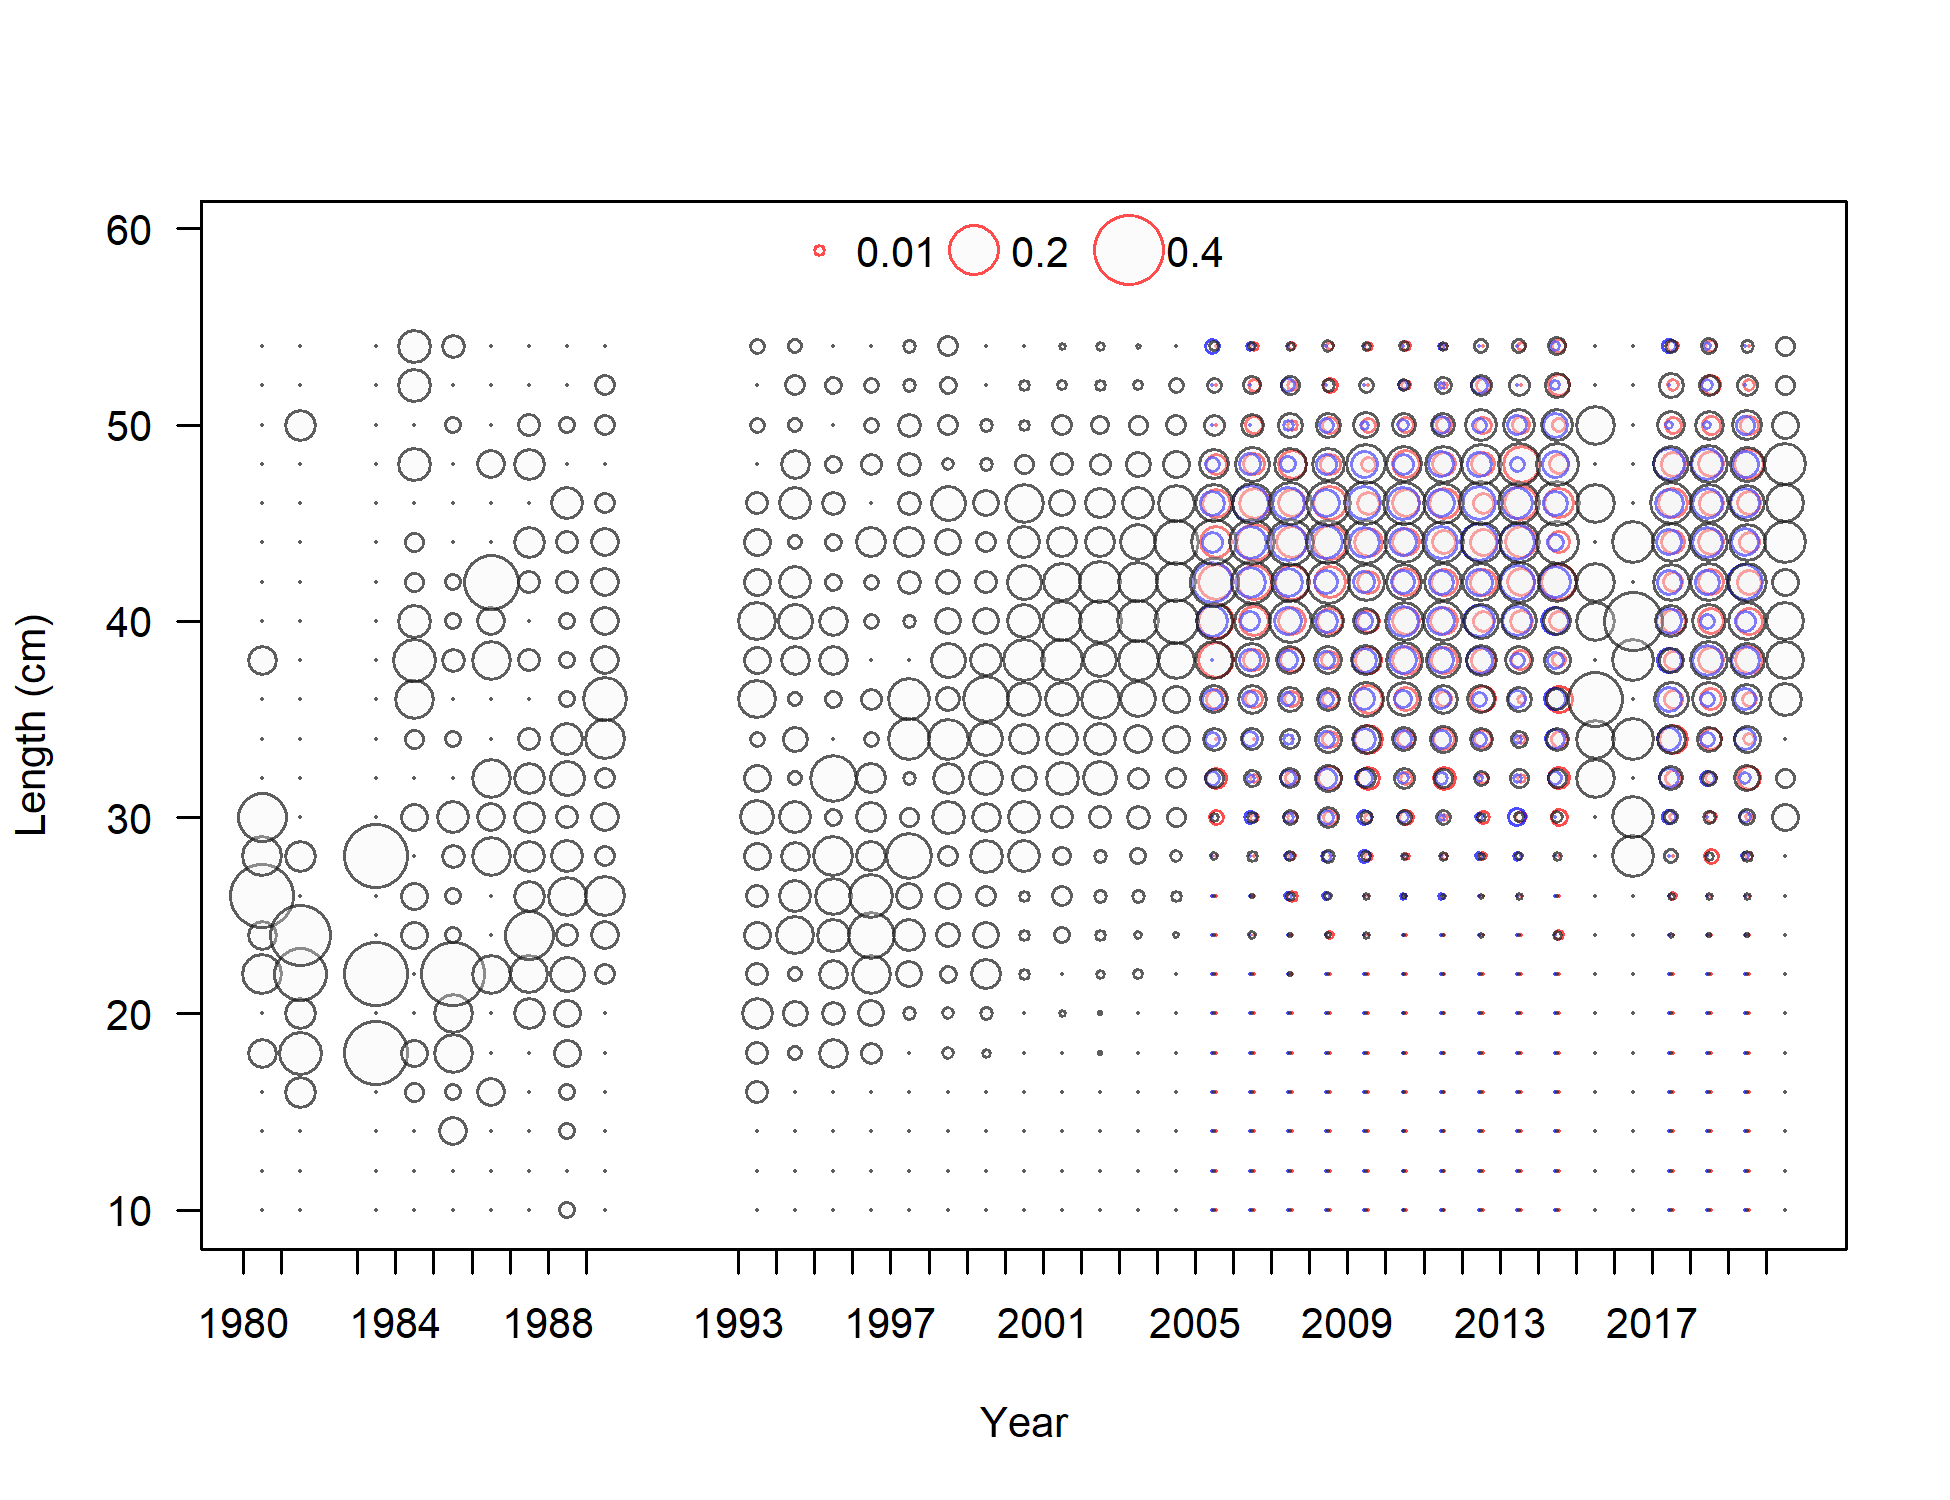
\includegraphics[width=1\textwidth,height=1\textheight]{C:/Users/Brian.Langseth/Desktop/or/7_1_0_base/plots/comp_lendat_bubflt2mkt0_page3.png}
\caption{Length composition data from the recreational fleet.\label{fig:rec-len-data}}
\end{figure}

\tagmcend\tagstructend

\tagstructbegin{tag=Figure,alttext={Mean length for recreational fleet with 95 percent confidence intervals.}}\tagmcbegin{tag=Figure}

\begin{figure}
\centering
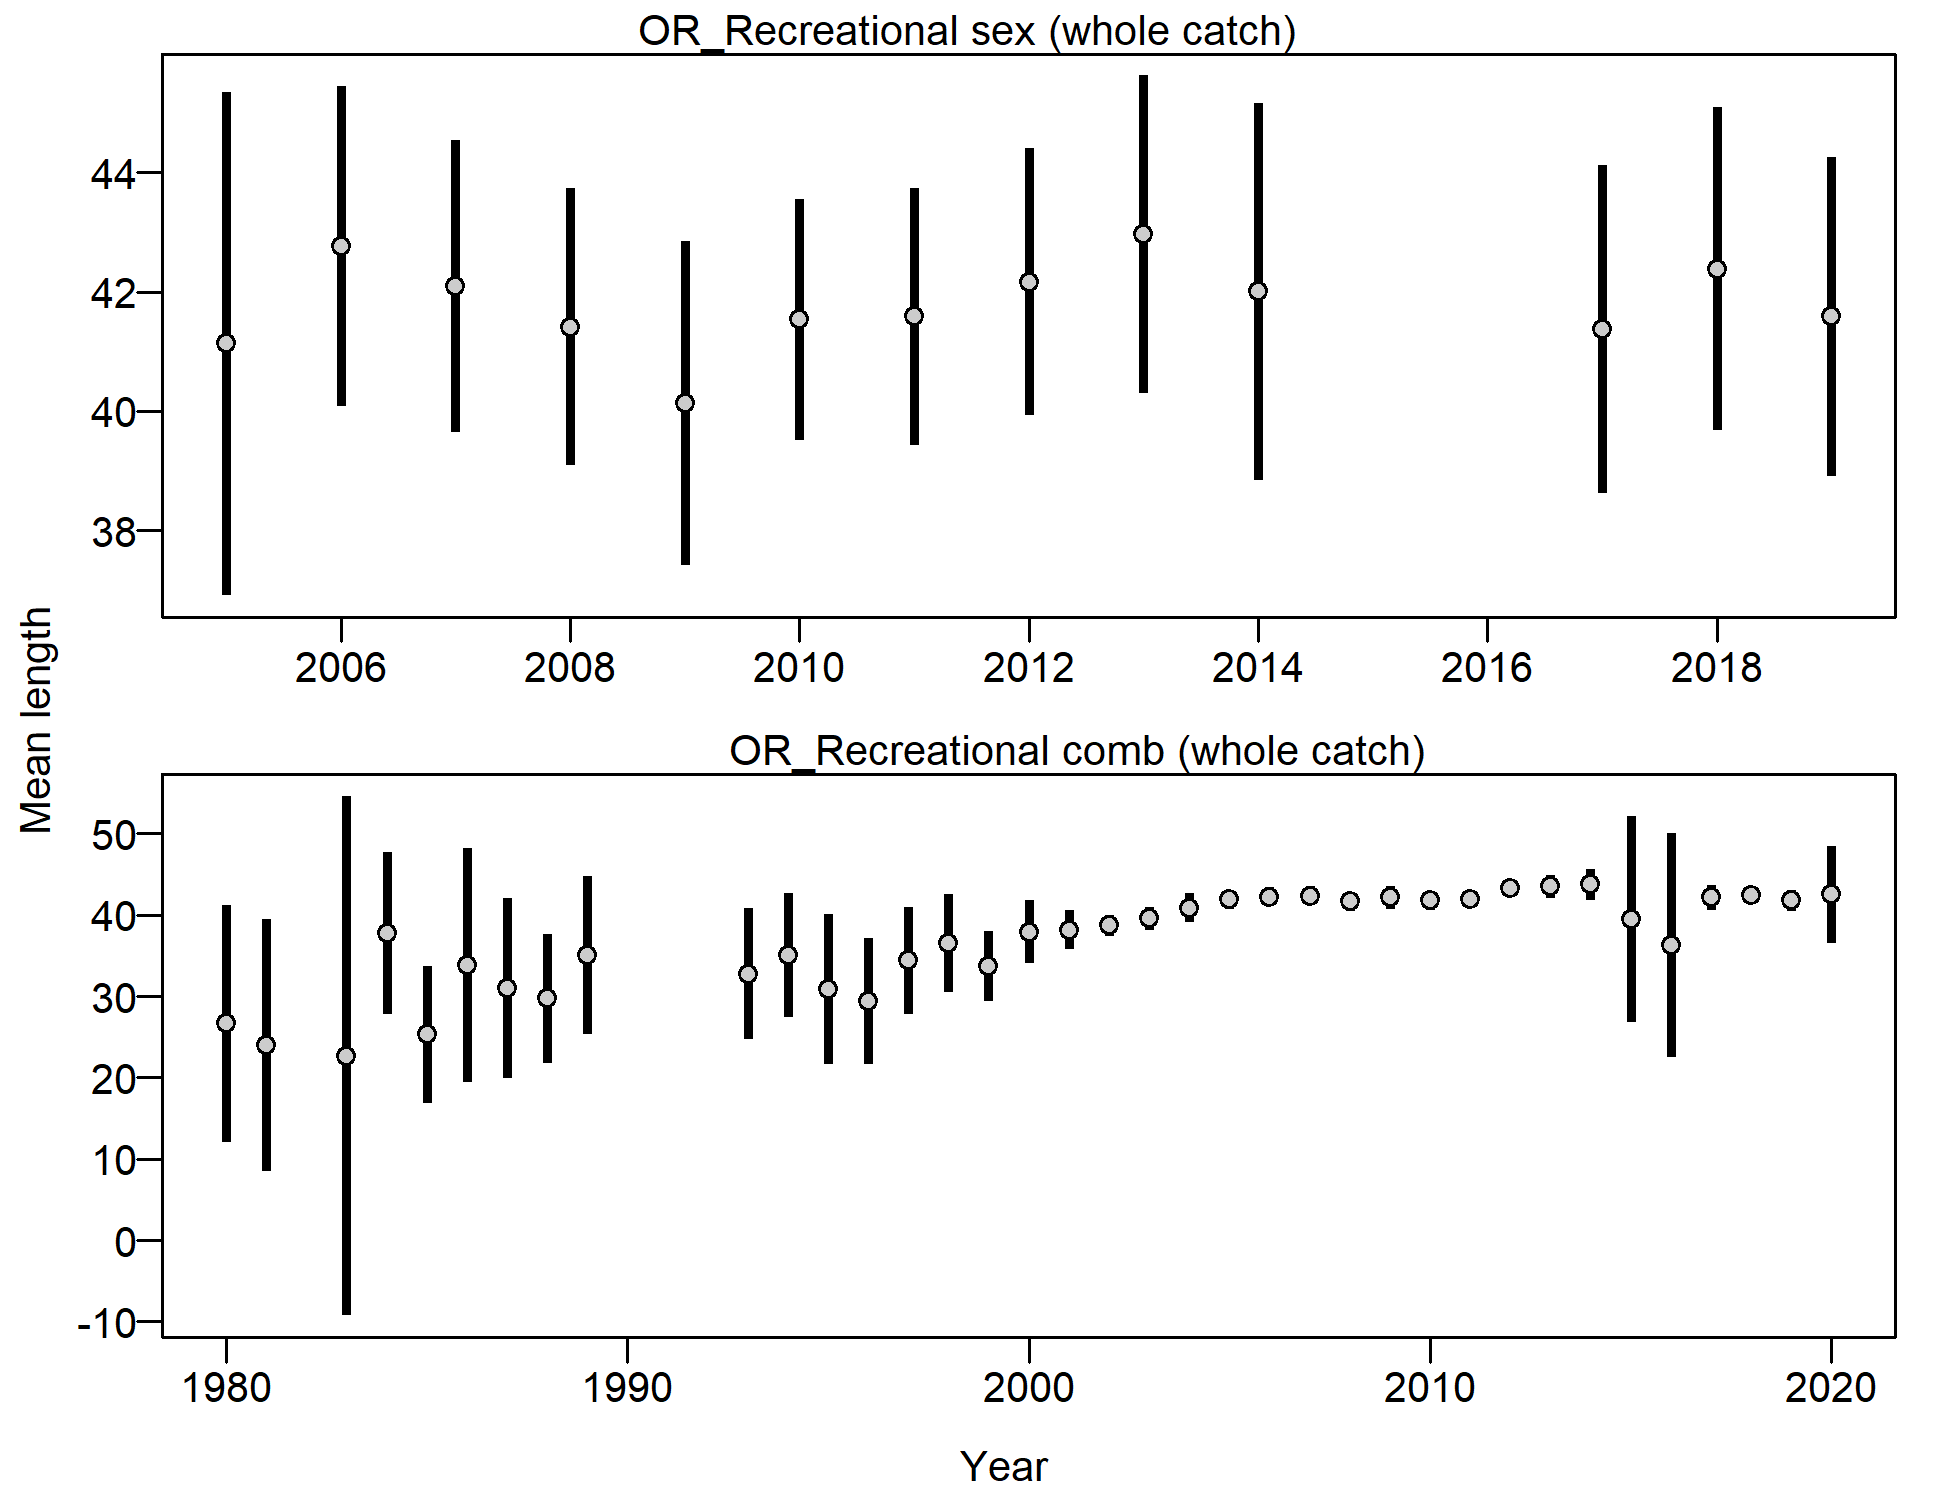
\includegraphics[width=1\textwidth,height=1\textheight]{C:/Users/Brian.Langseth/Desktop/or/7_1_0_base/plots/comp_lendat_data_weighting_TA1.8_OR_Recreational.png}
\caption{Mean length for recreational fleet with 95 percent confidence intervals.\label{fig:mean-rec-len-data}}
\end{figure}

\tagmcend\tagstructend

\tagstructbegin{tag=Figure,alttext={Maturity as a function of  length.}}\tagmcbegin{tag=Figure}

\begin{figure}
\centering
\includegraphics[width=1\textwidth,height=1\textheight]{C:/Users/Brian.Langseth/Desktop/or/7_1_0_base/plots/bio6_maturity.png}
\caption{Maturity as a function of length.\label{fig:maturity}}
\end{figure}

\tagmcend\tagstructend

\tagstructbegin{tag=Figure,alttext={Fecundity as a function of length.}}\tagmcbegin{tag=Figure}

\begin{figure}
\centering
\includegraphics[width=1\textwidth,height=1\textheight]{C:/Users/Brian.Langseth/Desktop/or/7_1_0_base/plots/bio9_fecundity_len.png}
\caption{Fecundity as a function of length.\label{fig:fecundity}}
\end{figure}

\tagmcend\tagstructend

\tagstructbegin{tag=Figure,alttext={Comparison of the length-at-weight data from the individual sources with length and weight data, and with all sources combined..}}\tagmcbegin{tag=Figure}

\begin{figure}
\centering
\includegraphics[width=1\textwidth,height=1\textheight]{//nwcfile/FRAM/Assessments/CurrentAssessments/DataModerate_2021/Quillback_Rockfish/data/output biology/plots/Length_Weight_by_Sex_ForReport.png}
\caption{Comparison of the length-at-weight data from the individual sources with length and weight data, and with all sources combined..\label{fig:len-weight-survey}}
\end{figure}

\tagmcend\tagstructend

\tagstructbegin{tag=Figure,alttext={Weight-at-length by sex used in the model.}}\tagmcbegin{tag=Figure}

\begin{figure}
\centering
\includegraphics[width=1\textwidth,height=1\textheight]{C:/Users/Brian.Langseth/Desktop/or/7_1_0_base/plots/bio5_weightatsize.png}
\caption{Weight-at-length by sex used in the model.\label{fig:len-weight}}
\end{figure}

\tagmcend\tagstructend

\tagstructbegin{tag=Figure,alttext={Observed sex specific length-at-age coastwide data by data source with the estimated length-at-age curve.}}\tagmcbegin{tag=Figure}

\begin{figure}
\centering
\includegraphics[width=1\textwidth,height=1\textheight]{//nwcfile/FRAM/Assessments/CurrentAssessments/DataModerate_2021/Quillback_Rockfish/data/output biology/plots/Length_Age_by_Sex_ForReport.png}
\caption{Observed sex specific length-at-age coastwide data by data source with the estimated length-at-age curve.\label{fig:len-age-data}}
\end{figure}

\tagmcend\tagstructend

\tagstructbegin{tag=Figure,alttext={Length at age in the beginning of the year in the ending year of the model.}}\tagmcbegin{tag=Figure}

\begin{figure}
\centering
\includegraphics[width=1\textwidth,height=1\textheight]{C:/Users/Brian.Langseth/Desktop/or/7_1_0_base/plots/bio1_sizeatage.png}
\caption{Length at age in the beginning of the year in the ending year of the model.\label{fig:len-age-ss}}
\end{figure}

\tagmcend\tagstructend

\tagstructbegin{tag=Figure,alttext={Selectivity at length by fleet.}}\tagmcbegin{tag=Figure}

\begin{figure}
\centering
\includegraphics[width=1\textwidth,height=1\textheight]{C:/Users/Brian.Langseth/Desktop/or/7_1_0_base/plots/sel01_multiple_fleets_length1.png}
\caption{Selectivity at length by fleet.\label{fig:selex}}
\end{figure}

\tagmcend\tagstructend

\tagstructbegin{tag=Figure,alttext={Estimated time series of age-0 recruits (1000s).}}\tagmcbegin{tag=Figure}

\begin{figure}
\centering
\includegraphics[width=1\textwidth,height=1\textheight]{C:/Users/Brian.Langseth/Desktop/or/7_1_0_base/plots/ts11_Age-0_recruits_(1000s)_with_95_asymptotic_intervals.png}
\caption{Estimated time series of age-0 recruits (1000s).\label{fig:recruits}}
\end{figure}

\tagmcend\tagstructend

\tagstructbegin{tag=Figure,alttext={Estimated time series of recruitment deviations.}}\tagmcbegin{tag=Figure}

\begin{figure}
\centering
\includegraphics[width=1\textwidth,height=1\textheight]{C:/Users/Brian.Langseth/Desktop/or/7_1_0_base/plots/recdevs2_withbars.png}
\caption{Estimated time series of recruitment deviations.\label{fig:rec-devs}}
\end{figure}

\tagmcend\tagstructend

\tagstructbegin{tag=Figure,alttext={Recruitment bias adjustment applied in the base model.}}\tagmcbegin{tag=Figure}

\begin{figure}
\centering
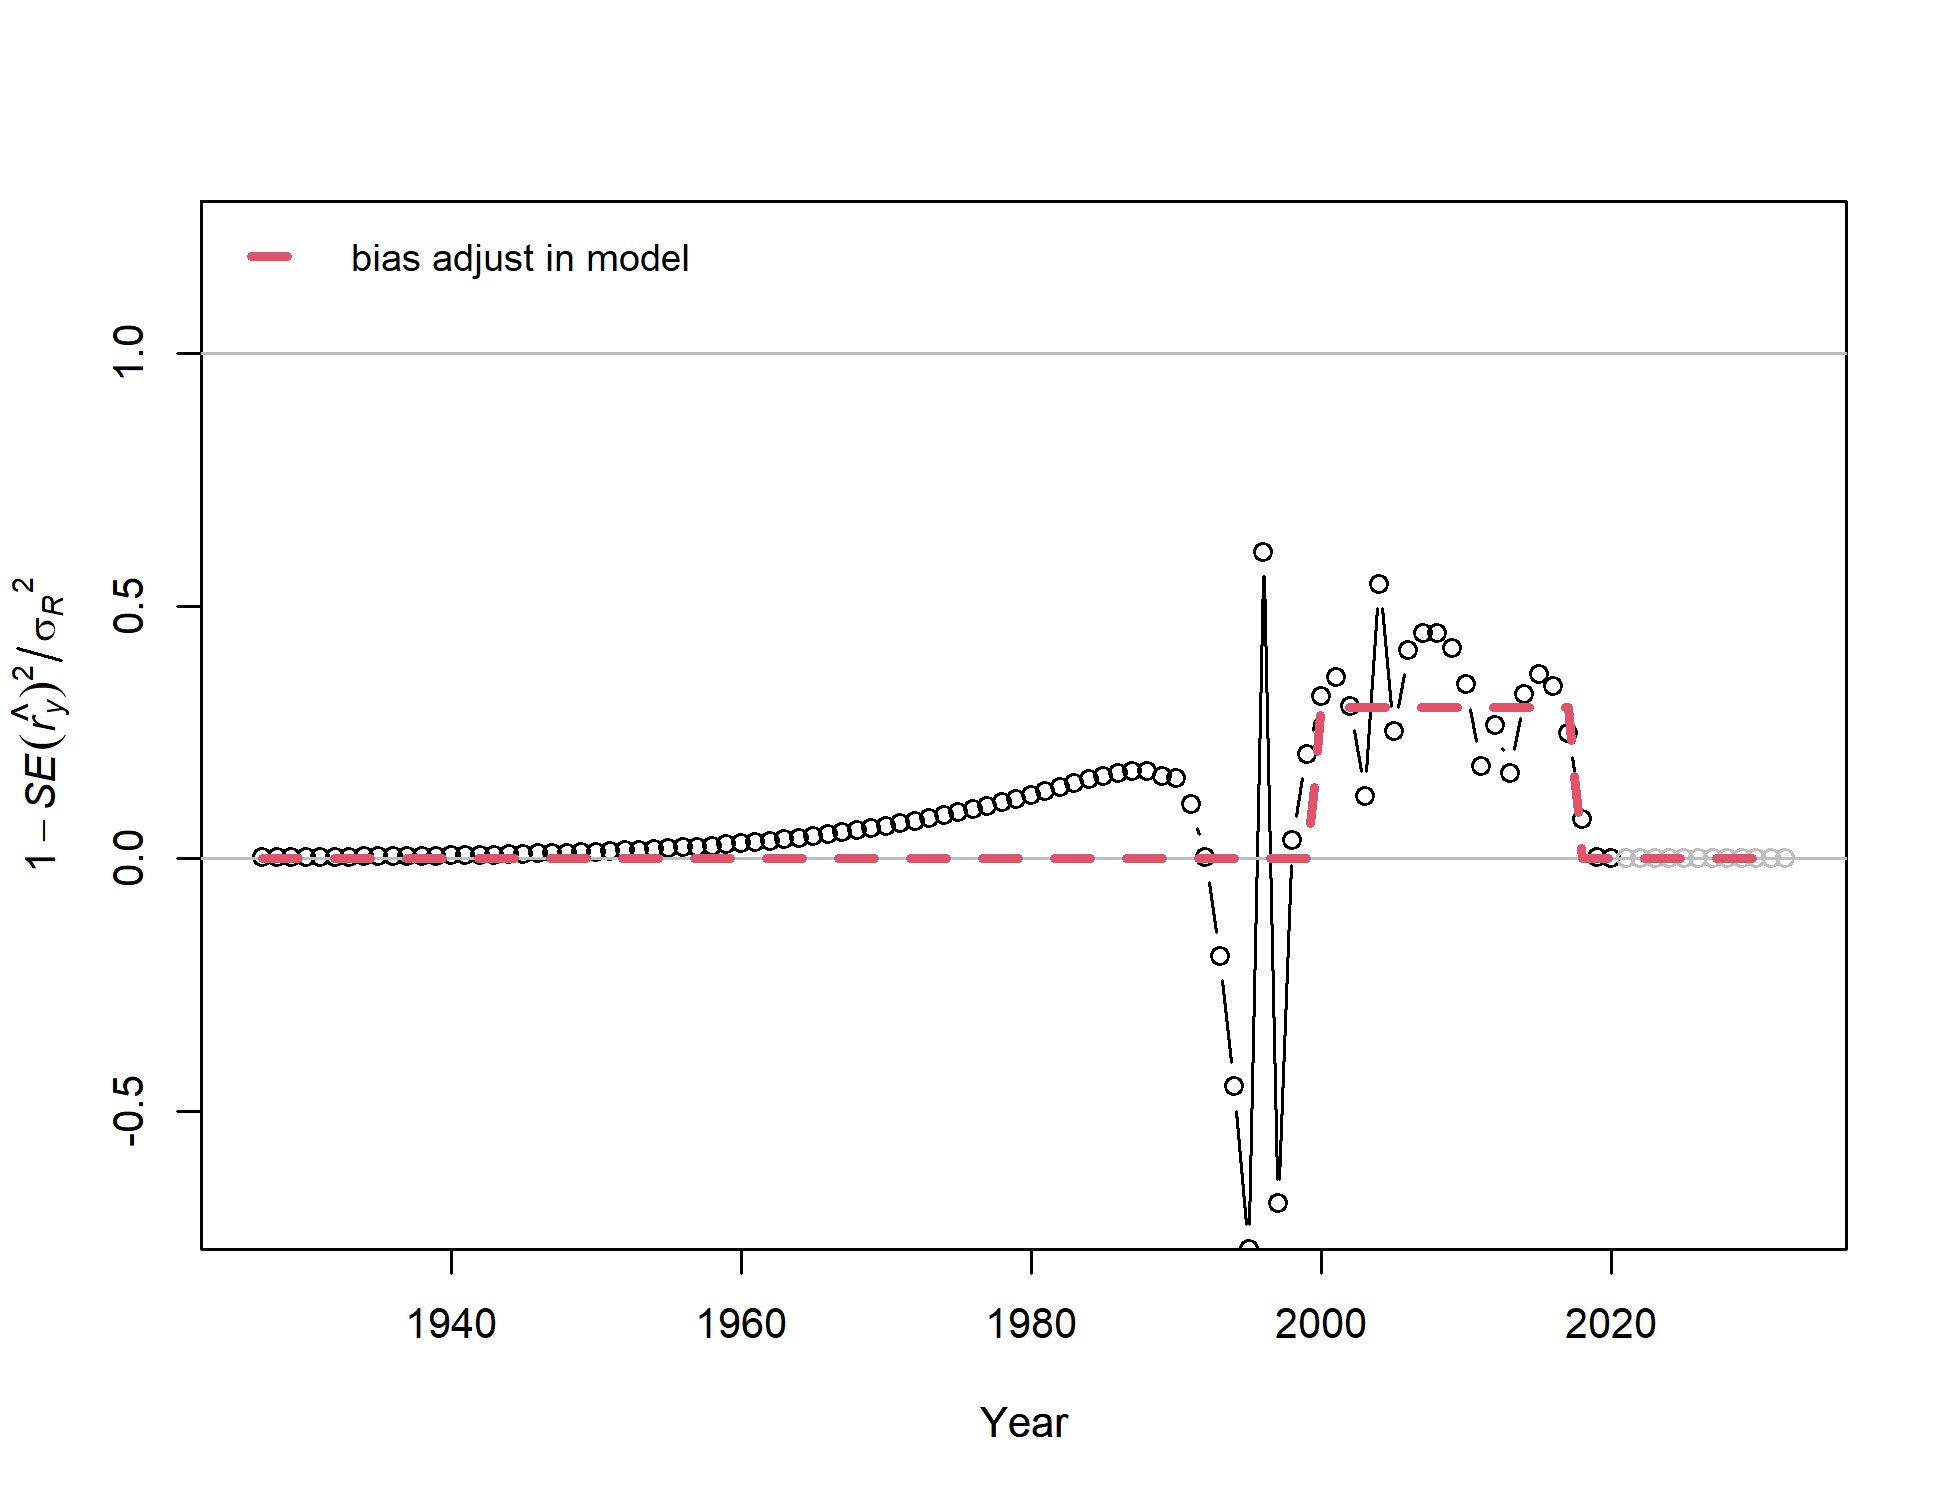
\includegraphics[width=1\textwidth,height=1\textheight]{C:/Users/Brian.Langseth/Desktop/or/7_1_0_base/plots/recruit_fit_bias_adjust.png}
\caption{Recruitment bias adjustment applied in the base model.\label{fig:bias-adj}}
\end{figure}

\tagmcend\tagstructend

\tagstructbegin{tag=Figure,alttext={Pearson residuals for commercial fleet. Closed bubble are positive residuals (observed > expected) and open bubbles are negative residuals (observed < expected).}}\tagmcbegin{tag=Figure}

\begin{figure}
\centering
\includegraphics[width=1\textwidth,height=1\textheight]{C:/Users/Brian.Langseth/Desktop/or/7_1_0_base/plots/comp_lenfit_residsflt1mkt0_page2.png}
\caption{Pearson residuals for commercial fleet. Closed bubble are positive residuals (observed \textgreater{} expected) and open bubbles are negative residuals (observed \textless{} expected).\label{fig:com-pearson}}
\end{figure}

\tagmcend\tagstructend

\tagstructbegin{tag=Figure,alttext={Model estimated mean length (blue line) overlaid on mean length of commercial lengths (gray circles) with 95 percent confidence intervals based on current samples sizes.}}\tagmcbegin{tag=Figure}

\begin{figure}
\centering
\includegraphics[width=1\textwidth,height=1\textheight]{C:/Users/Brian.Langseth/Desktop/or/7_1_0_base/plots/comp_lenfit_data_weighting_TA1.8_OR_Commercial.png}
\caption{Model estimated mean length (blue line) overlaid on mean length of commercial lengths (gray circles) with 95 percent confidence intervals based on current samples sizes.\label{fig:com-mean-len-fit}}
\end{figure}

\tagmcend\tagstructend

\tagstructbegin{tag=Figure,alttext={Pearson residuals for recreational fleet. Closed bubble are positive residuals (observed > expected) and open bubbles are negative residuals (observed < expected).}}\tagmcbegin{tag=Figure}

\begin{figure}
\centering
\includegraphics[width=1\textwidth,height=1\textheight]{C:/Users/Brian.Langseth/Desktop/or/7_1_0_base/plots/comp_lenfit_residsflt2mkt0_page3.png}
\caption{Pearson residuals for recreational fleet. Closed bubble are positive residuals (observed \textgreater{} expected) and open bubbles are negative residuals (observed \textless{} expected).\label{fig:rec-pearson}}
\end{figure}

\tagmcend\tagstructend

\tagstructbegin{tag=Figure,alttext={Model estimated mean length (blue line) overlaid on mean length for recreational lengths (gray circles) with 95 percent confidence intervals based on current samples sizes.}}\tagmcbegin{tag=Figure}

\begin{figure}
\centering
\includegraphics[width=1\textwidth,height=1\textheight]{C:/Users/Brian.Langseth/Desktop/or/7_1_0_base/plots/comp_lenfit_data_weighting_TA1.8_OR_Recreational.png}
\caption{Model estimated mean length (blue line) overlaid on mean length for recreational lengths (gray circles) with 95 percent confidence intervals based on current samples sizes.\label{fig:rec-mean-len-fit}}
\end{figure}

\tagmcend\tagstructend

\tagstructbegin{tag=Figure,alttext={Aggregated length comps over all years.}}\tagmcbegin{tag=Figure}

\begin{figure}
\centering
\includegraphics[width=1\textwidth,height=1\textheight]{C:/Users/Brian.Langseth/Desktop/or/7_1_0_base/plots/comp_lenfit__aggregated_across_time.png}
\caption{Aggregated length comps over all years.\label{fig:agg-len-fit}}
\end{figure}

\tagmcend\tagstructend

\tagstructbegin{tag=Figure,alttext={Estimated time series of spawning output (million of eggs).}}\tagmcbegin{tag=Figure}

\begin{figure}
\centering
\includegraphics[width=1\textwidth,height=1\textheight]{C:/Users/Brian.Langseth/Desktop/or/7_1_0_base/plots/ts7_Spawning_output_with_95_asymptotic_intervals_intervals.png}
\caption{Estimated time series of spawning output (million of eggs).\label{fig:ssb}}
\end{figure}

\tagmcend\tagstructend

\tagstructbegin{tag=Figure,alttext={Estimated time series of total biomass.}}\tagmcbegin{tag=Figure}

\begin{figure}
\centering
\includegraphics[width=1\textwidth,height=1\textheight]{C:/Users/Brian.Langseth/Desktop/or/7_1_0_base/plots/ts1_Total_biomass_(mt).png}
\caption{Estimated time series of total biomass.\label{fig:tot-bio}}
\end{figure}

\tagmcend\tagstructend

\tagstructbegin{tag=Figure,alttext={Estimated time series of relative spawning output.}}\tagmcbegin{tag=Figure}

\begin{figure}
\centering
\includegraphics[width=1\textwidth,height=1\textheight]{C:/Users/Brian.Langseth/Desktop/or/7_1_0_base/plots/ts9_Relative_spawning_output_intervals.png}
\caption{Estimated time series of relative spawning output.\label{fig:depl}}
\end{figure}

\tagmcend\tagstructend

\tagstructbegin{tag=Figure,alttext={Proportion of biomass unavailable due to selectivity for small and large fish..}}\tagmcbegin{tag=Figure}

\begin{figure}
\centering
\includegraphics[width=1\textwidth,height=1\textheight]{C:/Users/Brian.Langseth/Desktop/or/7_1_0_base/plots/UnavailableSpawningOutput.png}
\caption{Proportion of biomass unavailable due to selectivity for small and large fish..\label{fig:unavail-bio}}
\end{figure}

\tagmcend\tagstructend

\tagstructbegin{tag=Figure,alttext={Stock-recruit curve. Point colors indicate year, with warmer colors indicating earlier years and cooler colors in showing later years.}}\tagmcbegin{tag=Figure}

\begin{figure}
\centering
\includegraphics[width=1\textwidth,height=1\textheight]{C:/Users/Brian.Langseth/Desktop/or/7_1_0_base/plots/SR_curve.png}
\caption{Stock-recruit curve. Point colors indicate year, with warmer colors indicating earlier years and cooler colors in showing later years.\label{fig:bh-curve}}
\end{figure}

\tagmcend\tagstructend

\tagstructbegin{tag=Figure,alttext={Change in the negative log-likelihood across a range of log(R0) values.}}\tagmcbegin{tag=Figure}

\begin{figure}
\centering
\includegraphics[width=1\textwidth,height=1\textheight]{C:/Users/Brian.Langseth/Desktop/or/7_1_0_baseProfile_profile_SR_LN(R0)/piner_panel_SR_LN(R0).png}
\caption{Change in the negative log-likelihood across a range of log(R0) values.\label{fig:r0-profile}}
\end{figure}

\tagmcend\tagstructend

\tagstructbegin{tag=Figure,alttext={Change in the estimate of spawning output across a range of log(R0) values.}}\tagmcbegin{tag=Figure}

\begin{figure}
\centering
\includegraphics[width=1\textwidth,height=1\textheight]{C:/Users/Brian.Langseth/Desktop/or/7_1_0_baseProfile_profile_SR_LN(R0)/SR_LN(R0)_trajectories_compare1_spawnbio.png}
\caption{Change in the estimate of spawning output across a range of log(R0) values.\label{fig:r0-ssb}}
\end{figure}

\tagmcend\tagstructend

\tagstructbegin{tag=Figure,alttext={Change in the estimate of fraction unfished across a range of log(R0) values.}}\tagmcbegin{tag=Figure}

\begin{figure}
\centering
\includegraphics[width=1\textwidth,height=1\textheight]{C:/Users/Brian.Langseth/Desktop/or/7_1_0_baseProfile_profile_SR_LN(R0)/SR_LN(R0)_trajectories_compare3_Bratio.png}
\caption{Change in the estimate of fraction unfished across a range of log(R0) values.\label{fig:r0-depl}}
\end{figure}

\tagmcend\tagstructend

\tagstructbegin{tag=Figure,alttext={Change in the negative log-likelihood across a range of steepness values.}}\tagmcbegin{tag=Figure}

\begin{figure}
\centering
\includegraphics[width=1\textwidth,height=1\textheight]{C:/Users/Brian.Langseth/Desktop/or/7_1_0_baseProfile_profile_SR_BH_steep/piner_panel_SR_BH_steep.png}
\caption{Change in the negative log-likelihood across a range of steepness values.\label{fig:h-profile}}
\end{figure}

\tagmcend\tagstructend

\tagstructbegin{tag=Figure,alttext={Change in the estimate of spawning output across a range of steepness values.}}\tagmcbegin{tag=Figure}

\begin{figure}
\centering
\includegraphics[width=1\textwidth,height=1\textheight]{C:/Users/Brian.Langseth/Desktop/or/7_1_0_baseProfile_profile_SR_BH_steep/SR_BH_steep_trajectories_compare1_spawnbio.png}
\caption{Change in the estimate of spawning output across a range of steepness values.\label{fig:h-ssb}}
\end{figure}

\tagmcend\tagstructend

\tagstructbegin{tag=Figure,alttext={Change in the estimate of fraction unfished across a range of steepness values.}}\tagmcbegin{tag=Figure}

\begin{figure}
\centering
\includegraphics[width=1\textwidth,height=1\textheight]{C:/Users/Brian.Langseth/Desktop/or/7_1_0_baseProfile_profile_SR_BH_steep/SR_BH_steep_trajectories_compare3_Bratio.png}
\caption{Change in the estimate of fraction unfished across a range of steepness values.\label{fig:h-depl}}
\end{figure}

\tagmcend\tagstructend

\tagstructbegin{tag=Figure,alttext={Change in the negative log-likelihood across a range of female natural mortality values.}}\tagmcbegin{tag=Figure}

\begin{figure}
\centering
\includegraphics[width=1\textwidth,height=1\textheight]{C:/Users/Brian.Langseth/Desktop/or/7_1_0_baseProfile_profile_NatM_p_1_Fem_GP_1/piner_panel_NatM_p_1_Fem_GP_1.png}
\caption{Change in the negative log-likelihood across a range of female natural mortality values.\label{fig:m-profile}}
\end{figure}

\tagmcend\tagstructend

\tagstructbegin{tag=Figure,alttext={Change in the estimate of spawning output across a range of female natural mortality values.}}\tagmcbegin{tag=Figure}

\begin{figure}
\centering
\includegraphics[width=1\textwidth,height=1\textheight]{C:/Users/Brian.Langseth/Desktop/or/7_1_0_baseProfile_profile_NatM_p_1_Fem_GP_1/NatM_p_1_Fem_GP_1_trajectories_compare1_spawnbio.png}
\caption{Change in the estimate of spawning output across a range of female natural mortality values.\label{fig:m-ssb}}
\end{figure}

\tagmcend\tagstructend

\tagstructbegin{tag=Figure,alttext={Change in the estimate of fraction unfished across a range of female natural values.}}\tagmcbegin{tag=Figure}

\begin{figure}
\centering
\includegraphics[width=1\textwidth,height=1\textheight]{C:/Users/Brian.Langseth/Desktop/or/7_1_0_baseProfile_profile_NatM_p_1_Fem_GP_1/NatM_p_1_Fem_GP_1_trajectories_compare3_Bratio.png}
\caption{Change in the estimate of fraction unfished across a range of female natural values.\label{fig:m-depl}}
\end{figure}

\tagmcend\tagstructend

\tagstructbegin{tag=Figure,alttext={Change in the negative log-likelihood across a range of female maximum length values.}}\tagmcbegin{tag=Figure}

\begin{figure}
\centering
\includegraphics[width=1\textwidth,height=1\textheight]{C:/Users/Brian.Langseth/Desktop/or/7_1_0_baseProfile_profile_L_at_Amax_Fem_GP_1/piner_panel_L_at_Amax_Fem_GP_1.png}
\caption{Change in the negative log-likelihood across a range of female maximum length values.\label{fig:linf-profile}}
\end{figure}

\tagmcend\tagstructend

\tagstructbegin{tag=Figure,alttext={Change in the estimate of spawning output across a range of female maximum length values.}}\tagmcbegin{tag=Figure}

\begin{figure}
\centering
\includegraphics[width=1\textwidth,height=1\textheight]{C:/Users/Brian.Langseth/Desktop/or/7_1_0_baseProfile_profile_L_at_Amax_Fem_GP_1/L_at_Amax_Fem_GP_1_trajectories_compare1_spawnbio.png}
\caption{Change in the estimate of spawning output across a range of female maximum length values.\label{fig:linf-ssb}}
\end{figure}

\tagmcend\tagstructend

\tagstructbegin{tag=Figure,alttext={Change in the estimate of fraction unfished across a range of female maximum length values.}}\tagmcbegin{tag=Figure}

\begin{figure}
\centering
\includegraphics[width=1\textwidth,height=1\textheight]{C:/Users/Brian.Langseth/Desktop/or/7_1_0_baseProfile_profile_L_at_Amax_Fem_GP_1/L_at_Amax_Fem_GP_1_trajectories_compare3_Bratio.png}
\caption{Change in the estimate of fraction unfished across a range of female maximum length values.\label{fig:linf-depl}}
\end{figure}

\tagmcend\tagstructend

\tagstructbegin{tag=Figure,alttext={Change in the negative log-likelihood across a range of female k values.}}\tagmcbegin{tag=Figure}

\begin{figure}
\centering
\includegraphics[width=1\textwidth,height=1\textheight]{C:/Users/Brian.Langseth/Desktop/or/7_1_0_baseProfile_profile_VonBert_K_Fem_GP_1/piner_panel_VonBert_K_Fem_GP_1.png}
\caption{Change in the negative log-likelihood across a range of female k values.\label{fig:k-profile}}
\end{figure}

\tagmcend\tagstructend

\tagstructbegin{tag=Figure,alttext={Change in the estimate of spawning output across a range of female k values.}}\tagmcbegin{tag=Figure}

\begin{figure}
\centering
\includegraphics[width=1\textwidth,height=1\textheight]{C:/Users/Brian.Langseth/Desktop/or/7_1_0_baseProfile_profile_VonBert_K_Fem_GP_1/VonBert_K_Fem_GP_1_trajectories_compare1_spawnbio.png}
\caption{Change in the estimate of spawning output across a range of female k values.\label{fig:k-ssb}}
\end{figure}

\tagmcend\tagstructend

\tagstructbegin{tag=Figure,alttext={Change in the estimate of fraction unfished across a range of female k values.}}\tagmcbegin{tag=Figure}

\begin{figure}
\centering
\includegraphics[width=1\textwidth,height=1\textheight]{C:/Users/Brian.Langseth/Desktop/or/7_1_0_baseProfile_profile_VonBert_K_Fem_GP_1/VonBert_K_Fem_GP_1_trajectories_compare3_Bratio.png}
\caption{Change in the estimate of fraction unfished across a range of female k values.\label{fig:k-depl}}
\end{figure}

\tagmcend\tagstructend

\tagstructbegin{tag=Figure,alttext={Change in estimated spawning output by sensitivity.}}\tagmcbegin{tag=Figure}

\begin{figure}
\centering
\includegraphics[width=1\textwidth,height=1\textheight]{C:/Users/Brian.Langseth/Desktop/or/sensitivities/base.710_sensitivities_compare2_spawnbio_uncertainty.png}
\caption{Change in estimated spawning output by sensitivity.\label{fig:sens-ssb}}
\end{figure}

\tagmcend\tagstructend

\tagstructbegin{tag=Figure,alttext={Change in estimated fraction unfished by sensitivity.}}\tagmcbegin{tag=Figure}

\begin{figure}
\centering
\includegraphics[width=1\textwidth,height=1\textheight]{C:/Users/Brian.Langseth/Desktop/or/sensitivities/base.710_sensitivities_compare4_Bratio_uncertainty.png}
\caption{Change in estimated fraction unfished by sensitivity.\label{fig:sens-depl}}
\end{figure}

\tagmcend\tagstructend

\tagstructbegin{tag=Figure,alttext={Change in estimated annual recruitment deviation.}}\tagmcbegin{tag=Figure}

\begin{figure}
\centering
\includegraphics[width=1\textwidth,height=1\textheight]{C:/Users/Brian.Langseth/Desktop/or/sensitivities/base.710_sensitivities_compare12_recdevs_uncertainty.png}
\caption{Change in estimated annual recruitment deviation.\label{fig:sens-recdev}}
\end{figure}

\tagmcend\tagstructend

\tagstructbegin{tag=Figure,alttext={Change in the estimate of spawning output when the most recent 5 years of data area removed sequentially.}}\tagmcbegin{tag=Figure}

\begin{figure}
\centering
\includegraphics[width=1\textwidth,height=1\textheight]{C:/Users/Brian.Langseth/Desktop/or/7_1_0_baseProfile_retro/compare2_spawnbio_uncertainty.png}
\caption{Change in the estimate of spawning output when the most recent 5 years of data area removed sequentially.\label{fig:retro-ssb}}
\end{figure}

\tagmcend\tagstructend

\tagstructbegin{tag=Figure,alttext={Change in the estimate of fraction unfished when the most recent 5 years of data area removed sequentially.}}\tagmcbegin{tag=Figure}

\begin{figure}
\centering
\includegraphics[width=1\textwidth,height=1\textheight]{C:/Users/Brian.Langseth/Desktop/or/7_1_0_baseProfile_retro/compare4_Bratio_uncertainty.png}
\caption{Change in the estimate of fraction unfished when the most recent 5 years of data area removed sequentially.\label{fig:retro-depl}}
\end{figure}

\tagmcend\tagstructend

\tagstructbegin{tag=Figure,alttext={Estimated 1 - relative spawning ratio (SPR) by year.}}\tagmcbegin{tag=Figure}

\begin{figure}
\centering
\includegraphics[width=1\textwidth,height=1\textheight]{C:/Users/Brian.Langseth/Desktop/or/7_1_0_base/plots/SPR2_minusSPRseries.png}
\caption{Estimated 1 - relative spawning ratio (SPR) by year.\label{fig:1-spr}}
\end{figure}

\tagmcend\tagstructend

\tagstructbegin{tag=Figure,alttext={Equilibrium yield curve for the base case model. Values are based on the 2020 fishery selectivity and with steepness fixed at 0.72.}}\tagmcbegin{tag=Figure}

\begin{figure}
\centering
\includegraphics[width=1\textwidth,height=1\textheight]{C:/Users/Brian.Langseth/Desktop/or/7_1_0_base/plots/yield2_yield_curve_with_refpoints.png}
\caption{Equilibrium yield curve for the base case model. Values are based on the 2020 fishery selectivity and with steepness fixed at 0.72.\label{fig:yield}}
\end{figure}

\tagmcend\tagstructend

\newpage

\clearpage

\tagstructbegin{tag=H1}\tagmcbegin{tag=H1}

\hypertarget{appendix}{%
\section{Appendix}\label{appendix}}

\leavevmode\tagmcend\tagstructend

\tagstructbegin{tag=H2}\tagmcbegin{tag=H2}

\hypertarget{detailed-fit-to-length-composition-data}{%
\subsection{Detailed Fit to Length Composition Data}\label{detailed-fit-to-length-composition-data}}

\leavevmode\tagmcend\tagstructend

\tagstructbegin{tag=Figure,alttext={Length comps, whole catch, OR_Commercial (plot 1 of 2).<br><br>'N adj.' is the input sample size after data-weighting adjustment. N eff. is the calculated effective sample size used in the McAllister-Iannelli tuning method..}}\tagmcbegin{tag=Figure}

\begin{figure}
\centering
\includegraphics[width=1\textwidth,height=1\textheight]{C:/Users/Brian.Langseth/Desktop/or/7_1_0_base/plots/comp_lenfit_flt1mkt0_page1.png}
\caption{Length comps, whole catch, OR\_Commercial (plot 1 of 2).`N adj.' is the input sample size after data-weighting adjustment. N eff. is the calculated effective sample size used in the McAllister-Iannelli tuning method..\label{fig:comp_lenfit_flt1mkt0_page1}}
\end{figure}

\tagmcend\tagstructend

\tagstructbegin{tag=Figure,alttext={Length comps, whole catch, OR_Commercial (plot 2 of 2).}}\tagmcbegin{tag=Figure}

\begin{figure}
\centering
\includegraphics[width=1\textwidth,height=1\textheight]{C:/Users/Brian.Langseth/Desktop/or/7_1_0_base/plots/comp_lenfit_flt1mkt0_page2.png}
\caption{Length comps, whole catch, OR\_Commercial (plot 2 of 2).\label{fig:comp_lenfit_flt1mkt0_page2}}
\end{figure}

\tagmcend\tagstructend

\tagstructbegin{tag=Figure,alttext={Length comps, whole catch, OR_Recreational (plot 1 of 3).<br><br>'N adj.' is the input sample size after data-weighting adjustment. N eff. is the calculated effective sample size used in the McAllister-Iannelli tuning method..}}\tagmcbegin{tag=Figure}

\begin{figure}
\centering
\includegraphics[width=1\textwidth,height=1\textheight]{C:/Users/Brian.Langseth/Desktop/or/7_1_0_base/plots/comp_lenfit_flt2mkt0_page1.png}
\caption{Length comps, whole catch, OR\_Recreational (plot 1 of 3).`N adj.' is the input sample size after data-weighting adjustment. N eff. is the calculated effective sample size used in the McAllister-Iannelli tuning method..\label{fig:comp_lenfit_flt2mkt0_page1}}
\end{figure}

\tagmcend\tagstructend

\tagstructbegin{tag=Figure,alttext={Length comps, whole catch, OR_Recreational (plot 2 of 3).}}\tagmcbegin{tag=Figure}

\begin{figure}
\centering
\includegraphics[width=1\textwidth,height=1\textheight]{C:/Users/Brian.Langseth/Desktop/or/7_1_0_base/plots/comp_lenfit_flt2mkt0_page2.png}
\caption{Length comps, whole catch, OR\_Recreational (plot 2 of 3).\label{fig:comp_lenfit_flt2mkt0_page2}}
\end{figure}

\tagmcend\tagstructend

\tagstructbegin{tag=Figure,alttext={Length comps, whole catch, OR_Recreational (plot 3 of 3).}}\tagmcbegin{tag=Figure}

\begin{figure}
\centering
\includegraphics[width=1\textwidth,height=1\textheight]{C:/Users/Brian.Langseth/Desktop/or/7_1_0_base/plots/comp_lenfit_flt2mkt0_page3.png}
\caption{Length comps, whole catch, OR\_Recreational (plot 3 of 3).\label{fig:comp_lenfit_flt2mkt0_page3}}
\end{figure}

\tagmcend\tagstructend

\tagstructbegin{tag=Figure,alttext={Ghost length comps, whole catch, OR_Commercial.<br><br>'N adj.' is the input sample size after data-weighting adjustment. N eff. is the calculated effective sample size used in the McAllister-Iannelli tuning method..}}\tagmcbegin{tag=Figure}

\begin{figure}
\centering
\includegraphics[width=1\textwidth,height=1\textheight]{C:/Users/Brian.Langseth/Desktop/or/7_1_0_base/plots/comp_gstlenfit_flt1mkt0.png}
\caption{Ghost length comps, whole catch, OR\_Commercial.`N adj.' is the input sample size after data-weighting adjustment. N eff. is the calculated effective sample size used in the McAllister-Iannelli tuning method..\label{fig:comp_gstlenfit_flt1mkt0}}
\end{figure}

\tagmcend\tagstructend

\clearpage

\tagstructbegin{tag=H2}\tagmcbegin{tag=H2}

\hypertarget{odfw-marine-reserve-hook-and-line-survey}{%
\subsection{ODFW Marine Reserve Hook and Line Survey}\label{odfw-marine-reserve-hook-and-line-survey}}

\leavevmode\tagmcend\tagstructend

\tagstructbegin{tag=P}\tagmcbegin{tag=P}

One source of information that fell outside the bounds of the current PFMC Groundfish Terms of Reference for Data Moderate assessment is the ODFW Marine Reserve Hook and Line Survey. This data source to date has not been used in any West Coast groundfish stock assessments, but will likely be considered in select future full rockfish assessments (e.g., black rockfish). Given that this is an existing data source that may prove useful for future rockfish assessments, we wanted to provide an overall summary of this data source and the available data for quillback rockfish.

\leavevmode\tagmcend\tagstructend\par

\tagstructbegin{tag=P}\tagmcbegin{tag=P}

The Marine Reserve Program in the ODFW has routinely monitored state marine reserves (MR) and associated comparison areas (CA) since 2011. Data from the hook and line survey from 2011 - 2019 are presented in this summary. Surveys in 2011 and 2012 only visited a single site, Redfish Rocks. Surveys from 2013 -- 2019 include reserves and comparison areas from four sites: Redfish Rocks, Cape Falcon, Cape Perpetua and Cascade Head. Each of these four sites has a marine reserve and one to three comparison areas. Comparison areas are specifically selected for each marine reserve to be similar in location, habitat and depth to the reserve but are subject to fishing pressure. Not all sites are sampled in each year, due to both the gradual implementation of the reserve network and the available staff to execute surveys. Sites and areas sampled that are included in this dataset are below.

\leavevmode\tagmcend\tagstructend\par

\begingroup\fontsize{10}{12}\selectfont
\begingroup\fontsize{10}{12}\selectfont

\tagstructbegin{tag=Table}\tagmcbegin{tag=Table}
\begin{longtable}[t]{>{\raggedright\arraybackslash}p{2.2cm}>{\raggedright\arraybackslash}p{5.75cm}>{\raggedright\arraybackslash}p{3.5cm}>{\raggedright\arraybackslash}p{1.25cm}}
\caption{\label{tab:table-1}Sites and areas sampled by the Marine Reserve Program hook and line survey.}\\
\toprule
Site & Area & Years Sampled & Total Samples\\
\midrule
\endfirsthead
\caption[]{\label{tab:table-1}Sites and areas sampled by the Marine Reserve Program hook and line survey. \textit{(continued)}}\\
\toprule
Site & Area & Years Sampled & Total Samples\\
\midrule
\endhead

\endfoot
\bottomrule
\endlastfoot
Redfish Rocks & Humbug CA & 2011 – 2019 & 8\\
Redfish Rocks & Redfish Rocks MR & 2011 – 2019 & 8\\
Redfish Rocks & Orford Reef CA & 2014, 2015, 2017, 2019 & 4\\
Cape Falcon & CA Adjacent to Cape Falcon MR & 2014, 2015, 2017, 2019 & 4\\
Cape Falcon & Cape Falcon MR & 2014, 2015, 2017, 2019 & 4\\
Cape Falcon & Cape Meares CA & 2014, 2015, 2017, 2019 & 4\\
Cape Falcon & Three Arch Rocks CA & 2014, 2015, 2017, 2019 & 4\\
Cape Perpetua & CA Outside Cape Perpetua MR & 2016, 2018 & 2\\
Cape Perpetua & Cape Perpetua MR & 2013, 2014, 2017, 2018 & 4\\
Cape Perpetua & Postage Stamp CA & 2013, 2014, 2017, 2018 & 4\\
Cascade Head & Cape Foulweather CA & 2015, 2016, 2018 & 3\\
Cascade Head & Cascade Head MR & 2013 - 2016, 2018 & 5\\
Cascade Head & Cavalier CA & 2013, 2015, 2016, 2018 & 4\\
Cascade Head & Schooner Creek CA & 2013 - 2016, 2018 & 5\\*
\end{longtable}
\leavevmode\tagmcend\tagstructend\par
\endgroup{}
\endgroup{}

\tagstructbegin{tag=P}\tagmcbegin{tag=P}

A 500 meter square grid overlaid on the sampling area defines the sample units or cells. Cells are randomly selected within a marine reserve or comparison area for each sampling event. Three replicate drifts are executed in each cell. The specific location of the drifts within the cell is selected by the captain. Over time, cells without appropriate habitat for the focus species, mainly groundfish, have been removed from the selection procedures, and those presented in this dataset include only those that are currently ``active''. The number of cells visited in a day can vary slightly and range from three to five. Data are aggregated to the cell-day level.

\leavevmode\tagmcend\tagstructend\par

\tagstructbegin{tag=H3}\tagmcbegin{tag=H3}

\hypertarget{quillback-rockfish-summary}{%
\subsubsection{Quillback Rockfish Summary}\label{quillback-rockfish-summary}}

\leavevmode\tagmcend\tagstructend

\tagstructbegin{tag=P}\tagmcbegin{tag=P}

Of the 940 total-cell days at 14 areas, 164 (17.4 percent) of those had positive quillback rockfish catches with a total of 291 observations of quillback rockfish across all years and sites. The number of quillback rockfish caught ranged from 1 to 10 fish in a cell-day.

\leavevmode\tagmcend\tagstructend\par

\begingroup\fontsize{10}{12}\selectfont

\begin{landscape}\begingroup\fontsize{10}{12}\selectfont

\tagstructbegin{tag=Table}\tagmcbegin{tag=Table}
\begin{longtable}[t]{l>{\raggedright\arraybackslash}p{1cm}>{\raggedright\arraybackslash}p{1cm}>{\raggedright\arraybackslash}p{1cm}>{\raggedright\arraybackslash}p{1cm}>{\raggedright\arraybackslash}p{1cm}>{\raggedright\arraybackslash}p{1cm}>{\raggedright\arraybackslash}p{1cm}>{\raggedright\arraybackslash}p{1cm}>{\raggedright\arraybackslash}p{1cm}>{\raggedright\arraybackslash}p{1cm}}
\caption{\label{tab:table-2}Summary of number of catch cell days and positive observations of quillback rockfish.}\\
\toprule
 & 2011 & 2012 & 2013 & 2014 & 2015 & 2016 & 2017 & 2018 & 2019 & Total\\
\midrule
\endfirsthead
\caption[]{\label{tab:table-2}Summary of number of catch cell days and positive observations of quillback rockfish. \textit{(continued)}}\\
\toprule
 & 2011 & 2012 & 2013 & 2014 & 2015 & 2016 & 2017 & 2018 & 2019 & Total\\
\midrule
\endhead

\endfoot
\bottomrule
\endlastfoot
Number of Positive Catch Cell-Days & 5.000 & 5.000 & 23.000 & 30.000 & 26.000 & 22.000 & 17.000 & 16.000 & 20.000 & 164.000\\
Total Cell-Days & 44.000 & 52.000 & 97.000 & 141.000 & 167.000 & 112.000 & 103.000 & 116.000 & 108.000 & 940.000\\
Proportion of Positives & 0.114 & 0.096 & 0.237 & 0.213 & 0.156 & 0.196 & 0.165 & 0.138 & 0.185 & 0.174\\
Total Number of Copper Caught & 9.000 & 9.000 & 51.000 & 52.000 & 34.000 & 55.000 & 22.000 & 27.000 & 32.000 & 291.000\\*
\end{longtable}
\leavevmode\tagmcend\tagstructend\par
\endgroup{}
\end{landscape}
\endgroup{}

\tagstructbegin{tag=Figure,alttext={Frequency of positive quillback rockfish catches between 2011 - 2019.}}\tagmcbegin{tag=Figure}

\begin{figure}
\centering
\includegraphics[width=1\textwidth,height=1\textheight]{//nwcfile/FRAM/Assessments/CurrentAssessments/DataModerate_2021/Quillback_Rockfish/data/OR state surveys/fig_1_marine_hkl.png}
\caption{Frequency of positive quillback rockfish catches between 2011 - 2019.\label{fig:pos-hkl}}
\end{figure}

\tagmcend\tagstructend

\tagstructbegin{tag=P}\tagmcbegin{tag=P}

Areas differ in both geographic location and the level of fishing pressure experienced or allowed. Staff from the Marine Reserves Program suggested that the treatment (reserve vs.~comparison area) may not be a delineating factor for the catch of some species (e.g., cabezon) due to the recent implementation of the reserves. It was suggested that data could be aggregated to the site level, functioning at the level of a reef complex, to examine patterns at different locations along the coast. However, this may not be possible with the sample size available at some sites.

\leavevmode\tagmcend\tagstructend\par

\tagstructbegin{tag=P}\tagmcbegin{tag=P}

Observations of quillback rockfish were varied across sample sites and years. The number of observations of quillback rockfish was highest at Redfish Rocks (N = 118) and closely followed by Cape Perpetua (N = 108).

\leavevmode\tagmcend\tagstructend\par

\begingroup\fontsize{10}{12}\selectfont
\begingroup\fontsize{10}{12}\selectfont

\tagstructbegin{tag=Table}\tagmcbegin{tag=Table}
\begin{longtable}[t]{l>{\raggedright\arraybackslash}p{1.83cm}>{\raggedright\arraybackslash}p{1.83cm}>{\raggedright\arraybackslash}p{1.83cm}>{\raggedright\arraybackslash}p{1.83cm}>{\raggedright\arraybackslash}p{1.83cm}}
\caption{\label{tab:table-3}Summary of sampling effort by year and site combined with the positive observations of quillback rockfish.}\\
\toprule
Site & Year & Number of Positive Catch Cell Days & Total Cell Days & Proportion of Positives & Total Number of Quillback Rockfish Caught\\
\midrule
\endfirsthead
\caption[]{\label{tab:table-3}Summary of sampling effort by year and site combined with the positive observations of quillback rockfish. \textit{(continued)}}\\
\toprule
Site & Year & Number of Positive Catch Cell Days & Total Cell Days & Proportion of Positives & Total Number of Quillback Rockfish Caught\\
\midrule
\endhead

\endfoot
\bottomrule
\endlastfoot
Cape Falcon & 2014 & 0 & 18 & 0.000 & 0\\
 & 2015 & 3 & 51 & 0.059 & 4\\
 & 2017 & 1 & 47 & 0.021 & 1\\
 & 2019 & 3 & 42 & 0.071 & 6\\
 & Total & 7 & 158 & 0.044 & 11\\
Cape Perpetua & 2013 & 8 & 34 & 0.235 & 23\\
 & 2014 & 13 & 34 & 0.382 & 31\\
 & 2016 & 11 & 42 & 0.262 & 40\\
 & 2018 & 7 & 41 & 0.171 & 14\\
 & Total & 39 & 151 & 0.258 & 108\\
Cascade Head & 2013 & 4 & 35 & 0.114 & 5\\
 & 2014 & 6 & 43 & 0.140 & 7\\
 & 2015 & 12 & 59 & 0.203 & 15\\
 & 2016 & 10 & 63 & 0.159 & 14\\
 & 2018 & 9 & 75 & 0.120 & 13\\
 & Total & 41 & 275 & 0.149 & 54\\
Redfish Rocks & 2011 & 5 & 44 & 0.114 & 9\\
 & 2012 & 5 & 52 & 0.096 & 9\\
 & 2013 & 11 & 28 & 0.393 & 23\\
 & 2014 & 11 & 46 & 0.239 & 14\\
 & 2015 & 11 & 57 & 0.193 & 15\\
 & 2016 & 1 & 7 & 0.143 & 1\\
 & 2017 & 16 & 56 & 0.286 & 21\\
 & 2019 & 17 & 66 & 0.258 & 26\\
 & Total & 77 & 356 & 0.216 & 118\\*
\end{longtable}
\leavevmode\tagmcend\tagstructend\par
\endgroup{}
\endgroup{}

\tagstructbegin{tag=P}\tagmcbegin{tag=P}

Catch-per-unit-effort (CPUE) was calculated by the number of fish per angler hour. The number of anglers and hooks are standardized for each survey. Angler hours have been adjusted for non-fishing time (i.e., travel time, etc.).

\leavevmode\tagmcend\tagstructend\par

\tagstructbegin{tag=Figure,alttext={Quillback rockfish CPUE calculated based on positive values only.}}\tagmcbegin{tag=Figure}

\begin{figure}
\centering
\includegraphics[width=1\textwidth,height=1\textheight]{//nwcfile/FRAM/Assessments/CurrentAssessments/DataModerate_2021/Quillback_Rockfish/data/OR state surveys/fig_2_cpue_val.png}
\caption{Quillback rockfish CPUE calculated based on positive values only.\label{fig:fig-2}}
\end{figure}

\tagmcend\tagstructend

\tagstructbegin{tag=Figure,alttext={Quillback rockfish CPUE calculated based on all values.}}\tagmcbegin{tag=Figure}

\begin{figure}
\centering
\includegraphics[width=1\textwidth,height=1\textheight]{//nwcfile/FRAM/Assessments/CurrentAssessments/DataModerate_2021/Quillback_Rockfish/data/OR state surveys/fig_3_cpue.png}
\caption{Quillback rockfish CPUE calculated based on all values.\label{fig:fig-3}}
\end{figure}

\tagmcend\tagstructend

\tagstructbegin{tag=P}\tagmcbegin{tag=P}

Additional filtering may not be necessary, as the filtering for ``active'' cells has already likely removed any unsuitable sampling units, based on habitat, depth and local knowledge. Based on the annual proportion of positive cell-days and the relative rarity of quillback rockfish encounters, there are probably not enough data to move forward with a timeseries at a coastwide level. However, Redfish Rocks has been sampled in each year from 2011 - 2019, except for 2018. Though sample size is extremely limited, CPUE based on positive values at this site shows a variable and slightly declining trend from 2011 to 2015 followed by a slightly increasing trend from 2015 to 2020 for quillback rockfish. This differs from the trajectory from the base model in which shows a decline from 2016 to 2020 (Figure \ref{fig:tot-bio}).

\leavevmode\tagmcend\tagstructend\par

\tagstructbegin{tag=Figure,alttext={Quillback rockfish CPUE calculated at Redfish Rocks based on postive values only.}}\tagmcbegin{tag=Figure}

\begin{figure}
\centering
\includegraphics[width=1\textwidth,height=1\textheight]{//nwcfile/FRAM/Assessments/CurrentAssessments/DataModerate_2021/Quillback_Rockfish/data/OR state surveys/fig_4_redfish_cpue.png}
\caption{Quillback rockfish CPUE calculated at Redfish Rocks based on postive values only.\label{fig:fig-4}}
\end{figure}

\tagmcend\tagstructend

\tagstructbegin{tag=P}\tagmcbegin{tag=P}

When all sites and all values are included, quillback rockfish appear to have a relatively stable trend from 2011 -- 2019, with the annual mean CPUE oscillating around the long-term mean.

\leavevmode\tagmcend\tagstructend\par

\tagstructbegin{tag=Figure,alttext={Quillback rockfish relative CPUE across all sample sites and with all data values.}}\tagmcbegin{tag=Figure}

\begin{figure}
\centering
\includegraphics[width=1\textwidth,height=1\textheight]{//nwcfile/FRAM/Assessments/CurrentAssessments/DataModerate_2021/Quillback_Rockfish/data/OR state surveys/fig_5_relative_cpue.png}
\caption{Quillback rockfish relative CPUE across all sample sites and with all data values.\label{fig:fig-5}}
\end{figure}

\tagmcend\tagstructend

\tagstructbegin{tag=H3}\tagmcbegin{tag=H3}

\hypertarget{video-lander-population-estimate}{%
\subsubsection{Video Lander Population Estimate}\label{video-lander-population-estimate}}

\leavevmode\tagmcend\tagstructend

\tagstructbegin{tag=P}\tagmcbegin{tag=P}

Oregon Department of Fish and Wildlife (ODFW) provided density estimates and a range of estimated population abundances from underwater video lander data for quillback rockfish (Sebastes maliger). The lander data was collected over nine years by the ODFW and summarized in Rasmuson et al.~({\tagstructbegin{tag=Reference}\tagmcbegin{tag=Reference}(Rasmuson et al. 2020)\leavevmode\tagmcend\tagstructend}). This large dataset is made up of ten independent studies carried out in both nearshore rocky reefs coastwide as well as select reef structures offshore of the central coast of Oregon. Underwater video landers are stationary platforms consisting of one to three video cameras. Landers used in deeper water employ advanced lighting systems for optimal viewing of fish and benthic habitat. Ambient light is used in shallow surveys. The variability in detection range by depth is an important factor to consider when deriving fish density from lander data. Therefore, a series of abundance estimates were provided to inform the quillback rockfish assessment. Methods are summarized below but a more detailed document is available by ODFW upon request.

\leavevmode\tagmcend\tagstructend\par

\tagstructbegin{tag=P}\tagmcbegin{tag=P}

Variability in range (and therefore, area viewed) directly influences fish abundance; therefore, fish density estimates were calculated using five different estimates of range. These include the average range, the range +/- one standard deviation from the mean, and the maximum and minimum ranges. The area viewed is calculated using both the range and the horizontal field of view. This viewed area was then combined with fish count data to generate fish densities. Count data were provided from Rasmuson et al.~(2020). As expected, the viewed range has a large effect on the calculated density of the fish, with larger ranges resulting in a lower density of fish. Since there is no way to know which range model most accurately reflects the true density of fish, multiple range estimates were combined into a single density estimate using a weighted arithmetic mean. Although the arithmetic mean is simpler and more intuitive, the fact that the area viewed increases exponentially suggests a geometric mean may be more appropriate. As an alternative to the arithmetic mean, the geometric mean density was calculated in three different ways to address the zeros in the data. Abundance estimates (numbers of fish) were calculated by multiplying the density estimate by an estimate of the habitat area. Coastwide habitat area was limited to primary or secondary habitat containing hard substrate. The western boundary was defined as the 200 m contour based on the depth of the continental shelf-break. The eastern boundary was based on the shallowest lander observation for each species. Quillback rockfish were not observed on lander video in water \textless22 m, therefore the 20 m contour was used. It should be noted that while the depth range of the lander surveys conducted by ODFW extends to 212 m, the majority of lander surveys have been conducted in either nearshore rocky reefs or at Stonewall Bank RCA on the central Oregon coast.

\leavevmode\tagmcend\tagstructend\par

\tagstructbegin{tag=P}\tagmcbegin{tag=P}

Abundance estimates for the coastwide survey area are provided for quillback rockfish derived from each of the nine density estimates; five range models, the weighted arithmetic mean, and three weighted geometric mean methods. For quillback rockfish, density estimates ranged from 0.004 ± 0.029 (no. fish / m2 ± SD) from the maximum range method to 0.950 ± 1.366 for the third geometric mean method. The estimated habitat area was 1,840 thousands of km2. Abundance estimates ranged from 7.3 ± 53.5 (millions of fish ± SD) to 1,751 ± 2,519. Estimates of abundance from the five range models produced similar results to the weighted arithmetic mean, ranging from 7.3 ± 53.5 (millions of fish ± SD) for the maximum range to 36.9 ± 247.0 for the minimum range. These were generally considered more plausible than the results based on the geometric density means. Caveats to this abundance estimate are provided in the detailed document, but include considerations of the use of the lander dataset and the estimation of habitat area.

\leavevmode\tagmcend\tagstructend\par

\tagstructbegin{tag=H3}\tagmcbegin{tag=H3}

\hypertarget{rov-minimum-population-estimate}{%
\subsubsection{ROV minimum population estimate}\label{rov-minimum-population-estimate}}

\leavevmode\tagmcend\tagstructend

\tagstructbegin{tag=P}\tagmcbegin{tag=P}

The ODFW has conducted remotely-operated vehicle (ROV) surveys for nearly 20 years, targeting nearshore rocky reef habitats and associated fish and invertebrate assemblages. Oregon ROV survey methods, analyses, and data were subjected to an SSC methodology review in 2019 and were determined to be suitable for use in west coast stock assessments, subject to assessment authors' evaluation of suitability for particular stocks and specific data uses. Oregon ROV data were used to estimate a minimum abundance of quillback rockfish within a subset of the total available nearshore habitat, as a reference point for the assessment, though these data are not included directly in the assessment model. A summary of the methodology to develop this estimate follows, and a more detailed document is in development and available upon request by ODFW.

\leavevmode\tagmcend\tagstructend\par

\tagstructbegin{tag=P}\tagmcbegin{tag=P}

ROV data from 2010 -- 2019 were used for this abundance estimate, reflecting the period during which high-definition cameras were used. Sites were surveyed as funding and personnel allowed, and not all sites were surveyed in each year. Transect-level densities were aggregated by reef, regardless of year surveyed. Most transects were roughly 500m in length. These densities were derived from the rocky habitat portions of these transects only, excluding data from portions of transects over ``soft'' habitats (mud, sand, gravel). Total abundance (number of individuals) for the survey area was estimated by summing reef-level abundances. Each reef-level abundance was calculated as the weighted mean density of all transects conducted at the site across all years (weighted by the total view area of rock per transect) times the total area of mapped rock at the site within 20 -- 70m range.

\leavevmode\tagmcend\tagstructend\par

\tagstructbegin{tag=P}\tagmcbegin{tag=P}

The total abundance estimate for quillback rockfish for the rock-only transect density expansion is 136,828 +/- 90,971 (SD) individuals. The total area included in this abundance estimate is 134.8 km2, representing an estimated 74.8\% of total rocky habitat within 20 -- 70m in Oregon waters. A total of 490 transects were included in the calculation of the site-level mean densities. Several regions of potential quillback rockfish habitat along the Oregon coast were not included in this estimate due to a lack of survey data. In the study's 20 -- 70m depth range, the most important of these is the coast south of Port Orford which holds over half of the remaining unsurveyed rocky reef area. Outside the study's depth range, the most important missing rocky habitats are the shallows between 0 -- 20m, which are typically difficult to survey using an ROV, and the expansive deeper (\textgreater{} 70m) portion of Arago Reef. Given these factors, the abundance estimate presented above is likely a minimum population estimate and intended to provide a reference point only for the scale of the population size in a portion of Oregon's nearshore rocky habitat.

\leavevmode\tagmcend\tagstructend\par
\end{document}
